\documentclass[../main.tex]{subfiles}
\graphicspath{{\subfix{..}}}
\begin{document}
\chapter{Dualcalorimetric analysis with neutrino oscillation for Precision Measurement}
\label{sec:joint_fit}

\epigraph{``We demand rigidly defined areas of doubt and uncertainty!''}{Douglas Adams, The Hitchhiker’s Guide to the Galaxy}

\minitoc

% I)  Introduction globale.
% -------------------------------------
% ... Aborder les points suivants de manière succinte, pour donner une vision d'ensemble...
%
%     + JUNO est une expérience de physique de précision : il sera indispensable de comprendre très précisément les effets de reconstruction. C'est  d'autant  plus un défi que Juno emploie une technologie standard en physique des neutrinos (sphère ou cuve de scintillateur liquide  + PMT) mais l'amène dans une configuration extrême et inédite (très gros volume de scintillation, PMT de 30 pouces, etc...) où comprendre les effets de détection peut s'avérer difficile. Il est possible de rater quelque chose. Pouvoir comparer les données et résultats issus de deux systèmes indépendants, soumis à des problèmes différents, est donc précieux. C'est l'origine du dev de sPMT en plus des LPMT.
%
%     + L'importance cruciale de la maîtrise de la reconstruction : résolution à mieux que 3% et biais très inférieur à 1% sur la connaissance de la non linéarité sous peine d'incapacité à mesurer la NMO.
% Rappeler cet élément majeur : si on se trompe de 1%, on conclut à la mauvaise NMO. Utiliser la figure donnée dans la thèse de Yang pour appuyer ce point.
%
%    + Une source possible de non linéarité difficile à détecter à ce stade est la QNL. (Voir section suivante pour définition complète).
%
%     + La DC répond à cela. Elle interviendra notamment en fournissant des méthodes de calibration permettant de corriger la QNL. Ne pas en dire plus, ref these Yang.
%
%     + Plus generalement : Comparer deux systèmes pour détecter des problèmes sur la calibration ou la reco de l'un des deux. C'est ce que l'on fait dans cette thèse en comparant directement les résultats de la mesure des params d'oscillation.
%
%    + Une difficulté à étudier : la corrélation entre les deux systèmes : pas suffisant de comparer l'écart entre les valeurs centrales aux incertitudes individuelles. Nous proposons dans ce chapitre une exploration préliminaire testant différentes méthodes, en prédisant la sensibilité de ces méthodes à la présence QNL à divers degrés.
%
%   + Plan du chapitre.

JUNO is a high-precision neutrino oscillation experiment. To resolve the Neutrino Mass Ordering (NMO) with the required statistical significance, JUNO must be sensitive to the subtle spectral phase shift, on the order of a few percents, as illustrated in Figure \ref{fig:joint_fit:juno-spectrum-oscillation}. This phase shift manifests as a small difference between the Normal Ordering (NO) and Inverted Ordering (IO) spectra, which becomes even smaller after accounting for detection effects such as energy resolution smearing, non-linear detector responses, and background contamination, as shown in Figure \ref{fig:joint_fit:juno-ordering}.


This chapter is based on simulated data due to the unavailability of real JUNO data, which will only be available in 2025. The purpose of this analysis is to validate the methods and tools developed for dual calorimetry and neutrino oscillation measurements, ensuring that they are robust and ready for future real data.

Among other condition, a precise and complete understanding of the reconstruction and detector effects is crucial.
The challenge reside in the technology used in the detector, which, while based on well known technology: scintillator observed by PMT, is being deployed on a scale never seen before, in term of scintillator volume and  PMT size. Understanding every effects that goes in the detector can become extremely complicated. Any method to help detecting problems is therefore welcome.
Comparing the data and results obtained by two systems measuring the same events, but subject to different sources of error, is therefore precious. This is the purpose of the dual calorimetry techniques used in JUNO thanks to the existence of 2 PMT systems: the LPMT and SPMT systems.

The reconstruction of the IBD positron energy must be very performant: an unprecedented resolution of 3\% at 1 MeV \cite{juno_collaboration_juno_2022} is necessary to determine the NMO with the aimed significance.

Furthermore, an energy scale uncertainty below 1\% is essential to accurately assess the likelihood of the NO and IO hypotheses. If this uncertainty exceeds 1\%, systematic biases could distort the reconstructed spectra, potentially leading to the erroneous exclusion of the correct mass ordering hypothesis (NO or IO). For instance, a shift in the energy scale could mimic a phase shift between the spectra, making it possible to wrongly favor NO when IO is true, or vice versa. This effect has been studied in the introduction of Chapter 4 of \cite{han_dual_2021}.

Understanding all the effects influencing the detector response can be quite complex. Consequently, any methodologies that facilitate problem detection and validation of the reconstruction processes are essential for ensuring accurate results.

\begin{figure}[ht]
\centering
  \centering
  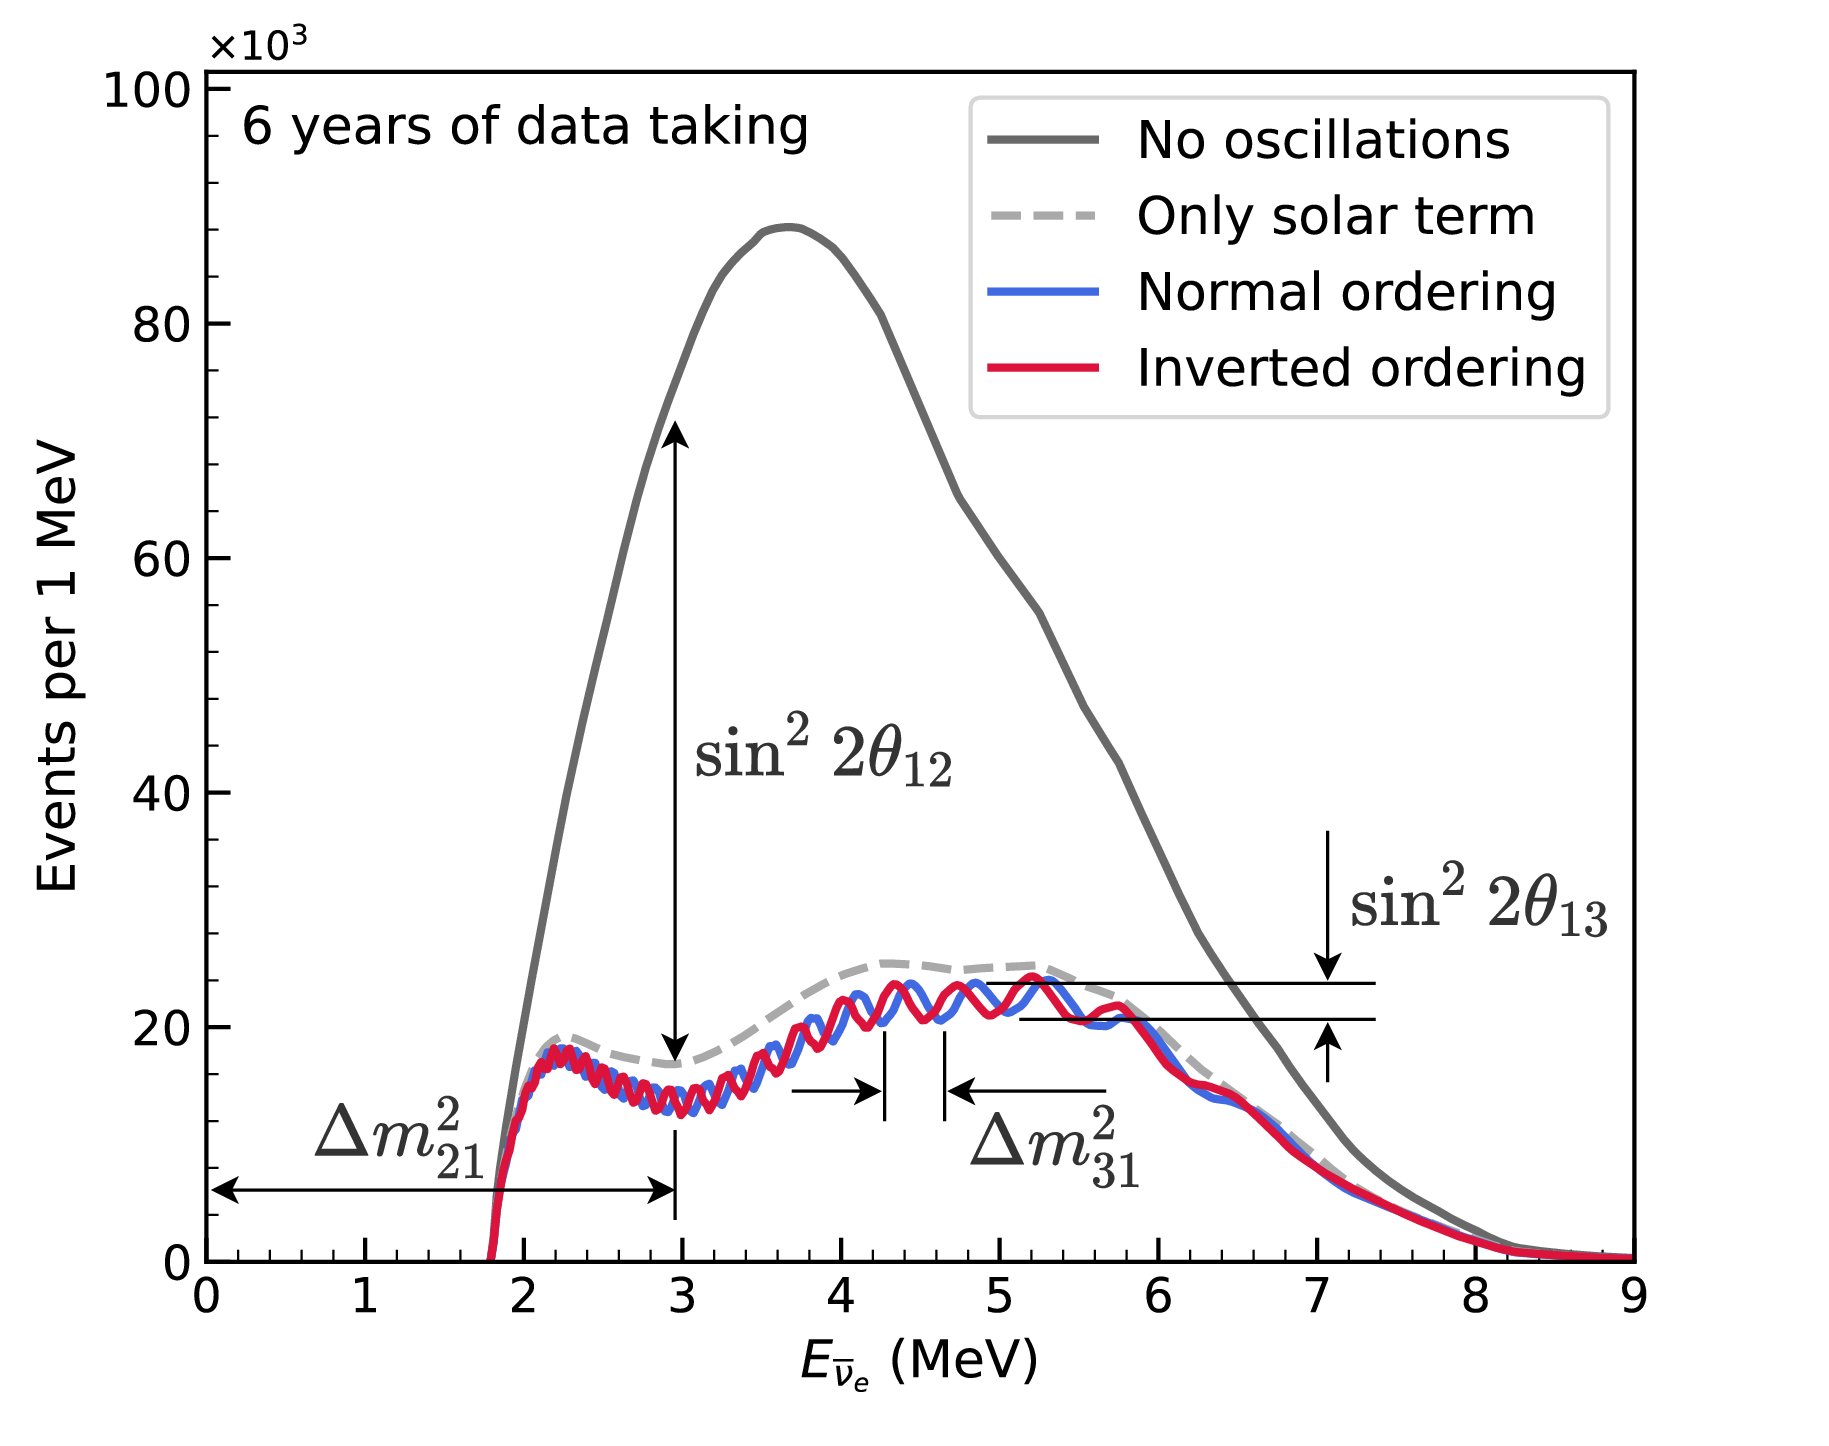
\includegraphics[height=6cm]{images/juno/Spectrum-OscillationsOnly_dm2_31.png}
  \caption{Expected number of neutrinos event per MeV in JUNO after 6 years of data taking. The black curve shows the flux if there was no oscillation. The light gray curve shows the oscillation if only the solar terms are taken in account ($\theta_{12}$, $\Delta m_{21}^2$). The blue and red curve shows the spectrum in the case of, respectively, NO and IO. The dependency of the oscillation to the different parameters are schematized by the double sided arrows. We can see the NMO sensitivity by looking at the fine phase shift between the red and the blue curve.}
  \label{fig:joint_fit:juno-spectrum-oscillation}
\end{figure}
\begin{figure}[ht]
  \centering
  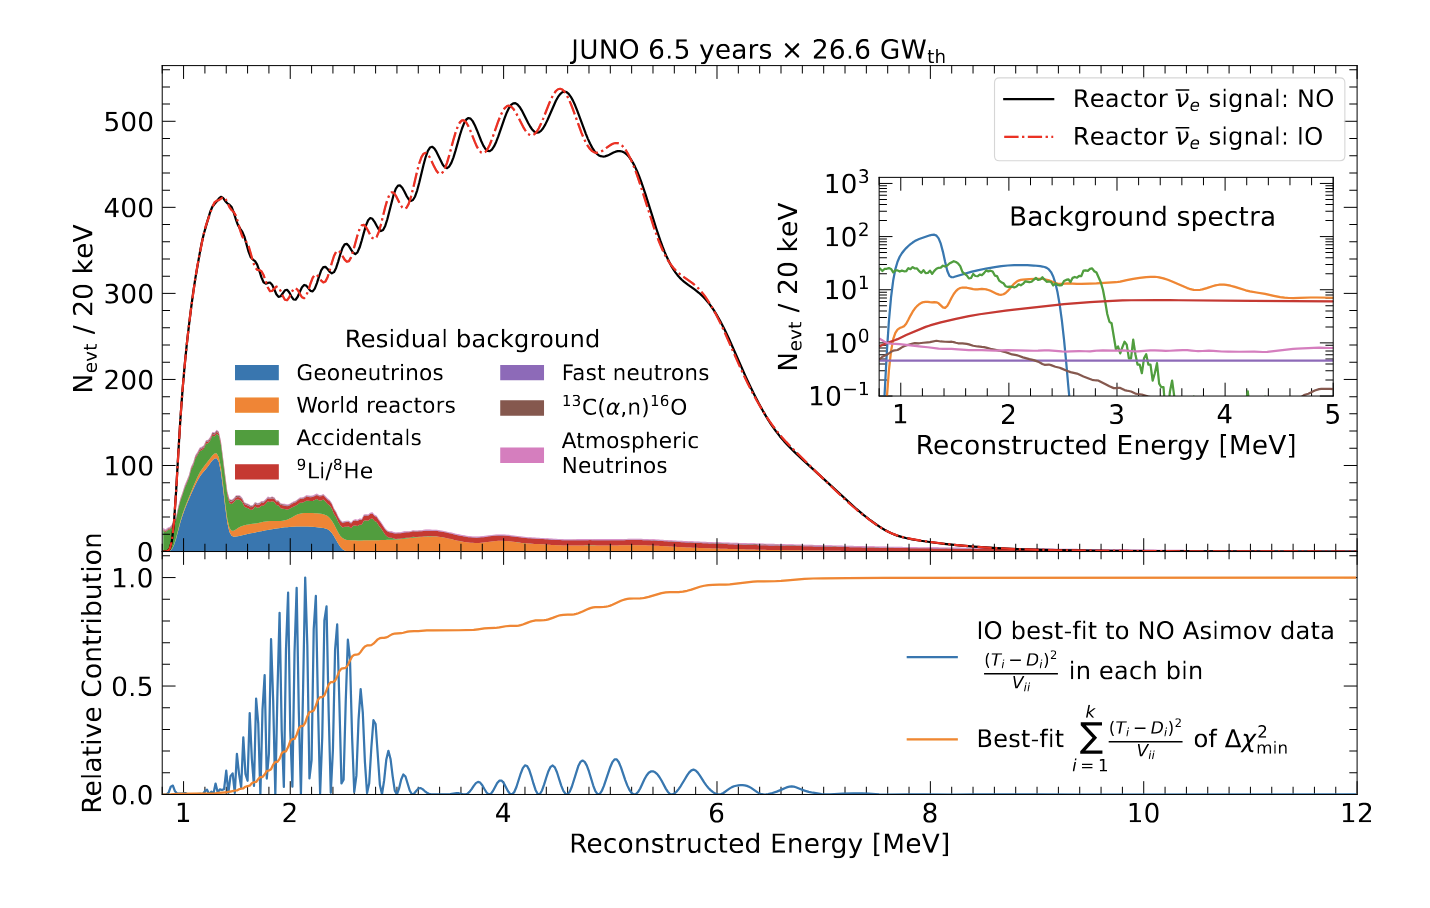
\includegraphics[height=8cm]{images/joint_fit/mass_ordering.png}
  \caption{Oscillated reactor $\bar{\nu}_e$ spectra for the Normal Ordering (Black) and Inverted Ordering (Red) for 6,5 years data taking and a resolution of 3\% without any statistical or systematic fluctuation. Figure from \cite{abusleme_potential_2024}.}
  \label{fig:joint_fit:juno-ordering}
\end{figure}

One detector effect to take into account is the detector  non linearity. Detector non-linearity can introduce significant biases in the energy reconstruction of events, compromising the precision of neutrino oscillation measurements and increasing systematic uncertainties, which could potentially distort the determination of the neutrino mass.

One of the possible source of non-linearity, which will be used as a reference in this chapter, is the charge non-linearity (QNL) that will be discussed in next section.
Several dual calorimetry techniques can address this issue. Some are calibration techniques, that are also described in section 4.3 of \cite{han_dual_2021} .
More generally, comparing the results of the two systems will allow for the detection of potential issues on the calibration or reconstruction. This is done in this thesis by comparing directly the spectra and oscillation parameters measurements of the two PMT systems. We call this kind of dual calorimetry "Dual calorimetry with neutrino oscillation", since it is based on the visible energy spectra used by the oscillation analysis of reactor antineutrinos.

In this chapter, we explore several ways to perform this comparison. One of them relies on the difference between the values of $\Delta m^2_{21}$, $\sin^2(2\theta_{12})$ measured with the LPMT and the SPMT systems.
Both systems measure them with similar uncertainties. For reasonable values of the QNL, we expect these differences to be smaller than the individual uncertainties. However, the significance of these differences might still be high. Indeed, both systems reconstruct the same events, therefore the same distribution of the true positron energy, as well as the same scintillation photon emission. Therefore,the energy spectra reconstructed by the two systems share a part of their fluctuations. This translates into correlated reconstructed spectra and consequently lead to correlations between the measurements of $\Delta m^2_{21}$ and $\sin^2(2\theta_{12})$. The uncertainty on the SPMT-LPMT difference is largely decreased by this correlation.  Other ways to perform the comparison
(see next sections) all rely the reconstructed spectra, therefore on the evaluation of the correlation between the LPMT and SPMT spectra.

In the next section we will discuss the motivations behind this study. In Section \ref{sec:joint_fit:approach},  I present the methods we propose to implement Dual calorimetry with neutrino oscillation, and of the way we estimate their sensitivity. In section \ref{sec:joint_fit:framework}, I present the fit framework used, and then, in section \ref{sec:joint_fit:tech} the technical improvement brought and the difficulties faced during the development. To end this chapter I present the results in \ref{sec:joint_fit:results} and discuss the conclusions and perspectives in \ref{sec:joint_fit:conclusion}.

\section{Motivations}
% II)  Motivations
% --------------------------
%
%   (a) Écart entre les résultats sPMT et LPMT
%       -- Tout écart significatif entre les résultats obtenus avec les deux systèmes signale un problème, et est donc intéressant, quelle que soit l'origine du problème.
%      -- Les deux systèmes ont une sensibilité équivalente à theta_12 et dm2_12. Ce sont donc ces deux paramètres que nous comparerons.
%     -- Pour détecter un écart significatif, on ne peut se contenter de comparer l'écart à la racine de la somme quad des erreurs individuelles. En effet, une grande partie de l'incertitude provient des incertitudes statistiques sur le spectre vrai de l'énergie des antineutrinos. Ce spectre étant le même pour les deux systèmes, les erreurs stats sur spectres reconstruits par les deux systèmes sont très corrélées. Si la reconstruction de l'E avait une résolution et un biais nul dans les deux systèmes, alors l'incertitude statistiques entre les mêmes bins des deux spectres serait 100% corrélée. Dans la réalité, les effets de reconstruction, en partie aléatoires, diminue cette corrélation. Elle reste néanmoins un élément central dans ce travail.
%
%    -- Notre travail dans cette partie de la thèse a été de mettre au point plusieurs tests statistiques pertinents pour détecter un écart entre le système des LPMT et celui des sPMT.
%      + Un premier objectif est de fournir les distributions des tests statistiques dans le cas où il n'existe pas de source de désaccord imprévue entre les deux systèmes. La valeur obtenue dans les données réelles pourra être comparée à ces distributions pour déduire des p-values.
%     + Pour évaluer une sensibilité, nous avons besoin de simuler une différence concrète. Nous choisissons de nous intéresser à un effet plausible, la QNL (voir prochaine sous-section). Nous soulignons cependant que la méthode peut être utile quelle que soit la source d'une différence entre LPMT et sPMT (problème dans la calibration, réglage fin de la simulation insuffisant pour un bon data/MC, etc...)
%
\subsection{Discrepancies between the SPMT and LPMT results}

As mentioned earlier, the SPMT and LPMT systems are expected to detect the same events. Therefore, after proper calibration, any significant discrepancies between the two systems' results could indicate a calibration error, a systematic effect, or an unaccounted detector issue. Detecting such differences is critical, as even small deviations from the expected response could compromise the determination of the Neutrino Mass Ordering (MO) or introduce systematic biases in the oscillation parameter measurements, leading to incorrect conclusions about the true mass ordering.

Both systems are anticipated to show similar sensitivity to the oscillation parameters $\theta_{12}$ and $\Delta m^2_{21}$ \cite{juno_collaboration_sub-percent_2022}. Therefore, any detected discrepancies will be based on these parameter measurements. A simple comparison of the values and independent uncertainties from the two systems could highlight discrepancies. However, we believe—and will demonstrate in this chapter—that an independent analysis of each system lacks critical information. By considering both statistical and systematic correlations between the two systems, we can design more robust and powerful statistical tests.

Our work in this chapter is to develop such tools, which in practice implies to define test statistics. A first step will be to determine the distribution of these test statistics in the case  when no unexpected problem affects the LPMT nor the SPMT problem. This will give us the distribution of those statistical test in absence of discrepancies. Later, the value of the test statistics that we will measure in real data can be compared to these distributions to produce p-values, to judge of the potential present of an unexpected effect.

To evaluate the power of our methods, we need to simulate a concrete difference between the two spectra.
We have chosen to study a specific potential effect, Charge Non-Linearity (QNL), which will be detailed in the following section. QNL affects the reconstructed energy spectrum by introducing a non-linear relationship between the true and measured charge in the PMTs. Our statistical tests are designed to detect such distortions, and they should be sensitive to unexpected effects—such as calibration errors or insufficient simulation precision—as long as the induced distortion exceeds a threshold of approximately 1-2\% in the reconstructed energy spectrum.

%
%   (b) Explications sur la QNL. (  ~ 1 p)
%
%       -- Rappeler que la réponse en E du détecteur est sujette à plusieurs sources de non linéarité. La principale est la NL dans la scintillation de photons. Une autre source est la QNL.
%
%      -- Définition, origine, etc.
%
%      -- Une façon de modéliser : la formule de Yang sur les Q_LPMT.
%          * Insérer les figures que tu as produites récemment (voir slack le 8 juillet à 17h39 et 17h52) : N_ph/N_ph_qnl vs. Etrue, pour différentes valeurs de gamma_qnl. Cela permet au lecteur de rapidement comprendre l'impact du PB.
%         * Fais le lien entre alpha_qnl et gamma_qnl, pour expliquer que plus tard, on ne testera que avec alpha_qnl, c'est à dire en simulant un effet global sur l'Erec pour générer plus vite.
%         * Dans ces figures, tu t'arrêtes à gamma_qnl = 1% <=> alpha_qnl = 0.3 %, je pense que tu peux aller jusqu'au 5% (regarde ce qui est fait chez Yang et dans la publi multicalo). Aussi bien à 0.5%, qu'à 1% et  qu'à 5%, donne le alpha_QNL correspondant, puis introduis-le dans IBDgen pour produire une spectre oscillé biaisé par la QNL, à comparer dans une figure au spectre sans QNL. Le but est de donner une idée de l'impact sur la NMO.
% En tout cas convaincre qu'il y en a un. Si Steven peut produire un delta-chi2, ce serait super.
%
% Remarques :
%       -- C'est un point important, donc il faut que cela soit auto-contenu au maximum.
%       -- S'inspirer de la publi multicalo, et de la thèse de Yang.
%       -- Citer ces deux sources, mais seulement en complément.
%

\subsection{Charge Non-Linearity (QNL)}
\label{sec:joint_fit:qnl}

The energy response of the Central Detector (CD) is influenced by two types of non-linearity. The first arises from the intrinsic properties of the Liquid Scintillator (LS), where the photon production is not linearly proportional to the deposited energy, as shown in Figure \ref{fig:juno:nl:gamma}. This non-linearity results from a combination of scintillation and Cherenkov light production. The scintillation yield is governed by Birk’s law, which introduces a "quenching" effect that depends on the particle type and energy. Additionally, Cherenkov radiation, which constitutes less than 10\% of the collected light, introduces a velocity-dependent non-linearity. These physical non-linearities in the LS contribute to the overall non-linearity of the energy response before any further distortions from the photomultiplier tubes (PMTs)

The second type of non-linearity comes from the LPMT charge measurements. When photons hit a PMT and give rise to PEs, a current pulse is formed. In the photon counting regime, simply exceeding a certain threshold allows to conclude that a single photon hit the PMT. When several photons hit the PMT simultaneously, one enters the photon integration regime : the pulse is sampled and integrated over a certain time window to produce a reconstructed charge Q. Calibration methods are applied to determine the relationship between the charge Q and the number of PEs (which is the quantity proportional to the energy deposit one wants to measure). Several effects impact this procedure: the signal pulse can fluctuate and be distorted between two events where the same number PEs occured; the PMT gain might not be linear as a function of the number of photons that hit the PMT; the charge reconstruction algorithm is not supposed to be perfect, and its results are further affected by electronic noise and inter-channel cross-talk. The impact of these effects grows with the number of PEs.

Precedent studies, Section 4.2.3 of \cite{han_dual_2021}, suggest a model for the channel-wise QNL:
\begin{equation}
  \label{eq:joint_fit:gamma_yang}
  \frac{Q_{rec}}{Q_{true}} = \frac{-\gamma_{qnl}}{9} Q_{true} + \frac{\gamma_{qnl} + 9}{9}
\end{equation}
where $Q_{rec}$ is the reconstructed number of PE by the PMT, $Q_{true}$ is true number of PE that hit the PMT, and $\gamma_{qnl}$ is a factor representing the amplitude of the non-linearity.

Studies at previous experiments, like Daya Bay, concluded that the best reachable control of QNL in the 1-10 PEs range was $\gamma_{qnl}=0.01$ \cite{collaboration_high_2019}.
As already mentionned in Section \ref{sec:juno:LPMT}, JUNO LPMTs operate in a larger range : 1-100 PEs (See also table \ref{tab:joint_fit:charge_frac}). In such a case, a realistic value of $\gamma_{qnl}$ is not known.

\begin{table}[ht]
  \centering
  \begin{tabular}{c|c|c|c|c|c|c|c}
        &1PE &2$\sim$5PE& 5$\sim$10PE & 10$\sim$20PE & 20$\sim$50PE & 50$\sim$100PE & >100PE \\
      \hline
    LPMT &42.56\% & 40.54\% & 8.74\% & 5.12\% & 2.80\% & 0.24\% & 0.003\% \\
    SPMT &95.19\% & 4.80\%  & 0.01\% & 0\%    & 0\%    & 0\%    & 0\% \\
    \hline
  \end{tabular}
  \caption{The charge fraction in terms of the number of PE collected at the single PMT for the reactor $\bar{\nu}_e$ IBD events. Table taken from \cite{han_dual_2021}}
  \label{tab:joint_fit:charge_frac}
\end{table}

The event-wise impact resulting from the channel-wise QNL can be parameterised this way :
\begin{equation}
  \label{eq:joint_fit:alpha_yang}
  \frac{E^{rec}_{vis}}{E^{true}_{vis}} = \frac{-\alpha_{qnl}}{9} E^{true}_{vis} + \frac{\alpha_{qnl} + 9}{9}
\end{equation}
In JUNO, the visible energy is proportional to the number of emitted photons per unit energy deposit. It includes the physical non linearities.
In the equation above $E_{vis}^{true}$ is this visible energy, while $E_{vis}^{rec}$ is what it becomes when the reconstructed charges found in an event are modified according to Eq. \ref{eq:joint_fit:gamma_yang}.

An example is shown on Fig. \ref{fig:juno:instr_nl}, where we show the $E^{rec}_{vis}/E_{true}^{vis}$ ratio for several samples of uniformly distributed electron events, generated with various values of $E_{true}^{vis}$.
Here, an extreme value $\gamma_{qnl}=0.05$ was assumed. On can see on Fig. \ref{fig:juno:instr_nl} that it corresponds to a 2\% effect at 8 MeV, equivalent to $\alpha_{qnl} = 0.025$. The effect of Eq \ref{eq:joint_fit:alpha_yang} is illustrated in Figure \ref{fig:joint_fit:spectrums_comp}.

\begin{figure}[ht]
  \centering
  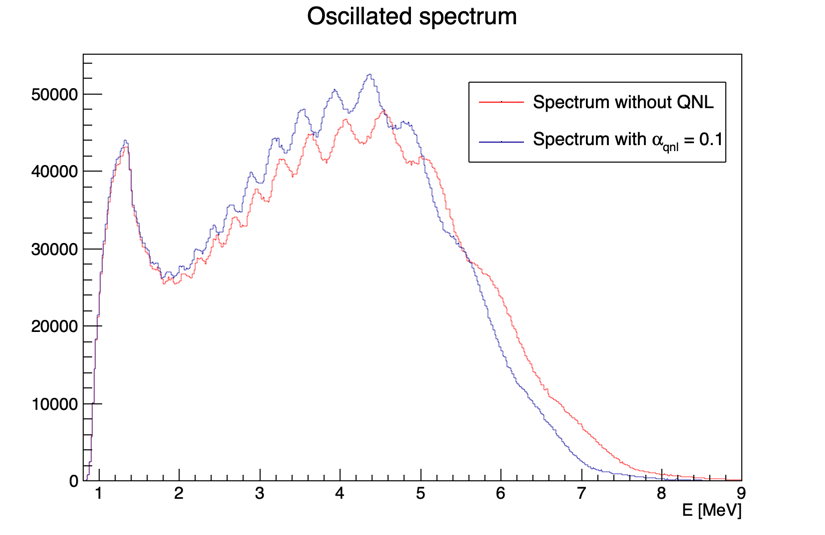
\includegraphics[height=5cm]{images/joint_fit/spectrums.png}
  \caption{\textbf{On top:} Oscillated spectra for different value of $\alpha_{qnl}$. \textbf{On bottom:} Ratio of the number of event with $\alpha_{qnl} = 0\%$.}
  \label{fig:joint_fit:spectrums_comp}
\end{figure}

This example is from  from references \cite{han_dual_2021}, which aimed at demonstrating the potential of the dual calorimetry calibration method mentioned in section
\ref{sec:juno:instr_nl}. If it works as hoped, the residual event-wise QNL effect will be below 0.3\%. In this chapter, we propose methods todetect residuals higher than this.

Fig. \ref{fig:joint_fit:gamma_v_alpha} show several other examples with varying $\gamma_{qnl}$ values, and the corresponding values of $\alpha_{qnl}$.
Using 1M events from the JUNO official simulation J23.0.1-rc8.dc1 (released on 7th January 2024), we
simulated events up to the photon collection in LPMTs and introduced an additional channel-wise
QNL by using the equation 7.1 to modify the number of collected photons.

\begin{figure}[ht]
  \centering
  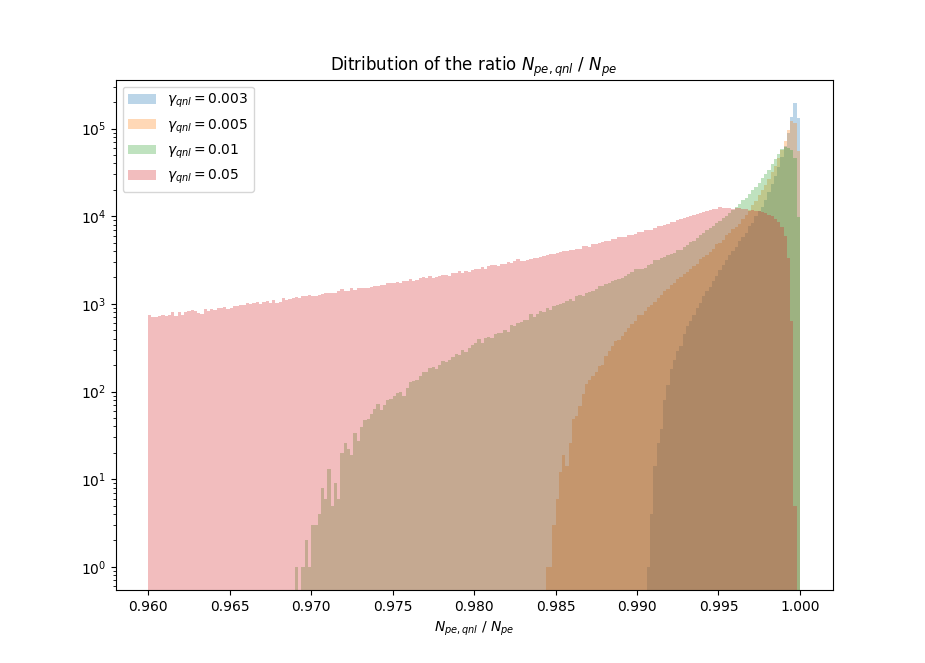
\includegraphics[height=6cm]{images/joint_fit/gamma_eff.png}
  \caption{Distribution the ratio reconstructed charge (in nPE equivalent) over the number of collected nPE for different value of $\gamma_{qnl}$. We use a sample of 1 million positron event uniformly distributed in the detector and in energy in the range $E_{dep} \in [1, 10] MeV$}
  \label{fig:joint_fit:ratio_distrib}
\end{figure}
\begin{figure}[ht]
  \centering
  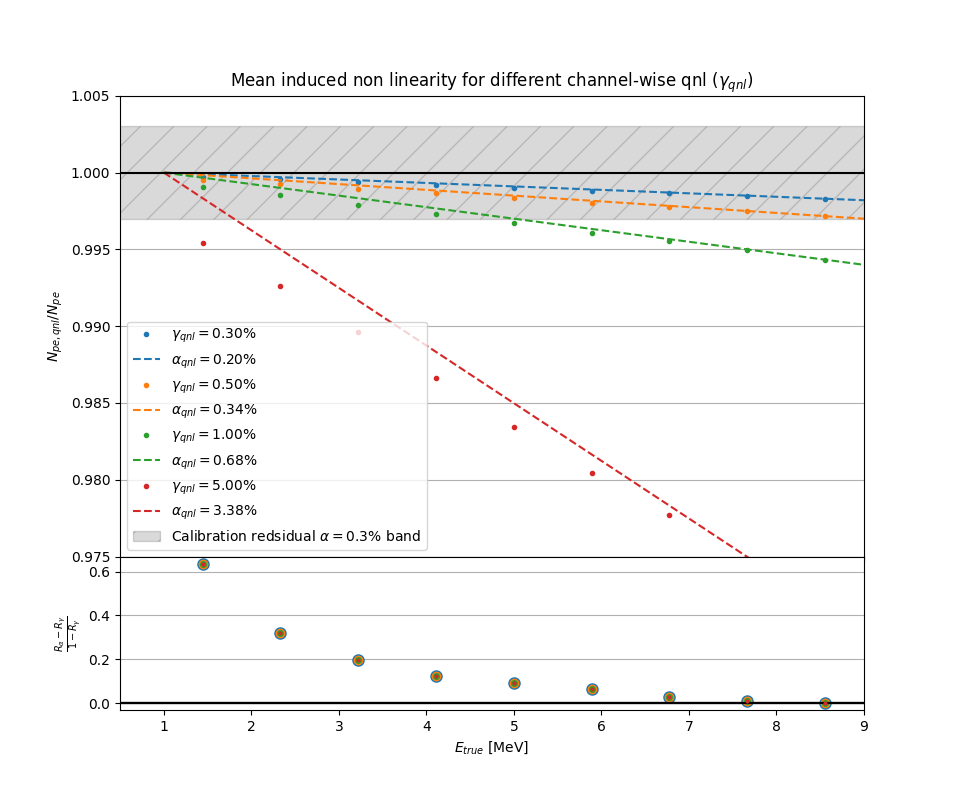
\includegraphics[height=8cm]{images/joint_fit/gamma_to_alpha.png}
  \caption{\textbf{On top:} Ratio of the reconstructed charge (in nPE equivalent) over the number of collected nPE. The dots represent the mean of the distributions in Figure \ref{fig:joint_fit:ratio_distrib} and the dashed line are the equivalent event-wise non-linearity from eq \ref{eq:joint_fit:alpha_yang}. The hatched zone is the residual non-linearity expected after calibration \cite{juno_collaboration_calibration_2021}. \textbf{On bottom:} Difference between QNL induced by an event wise QNL and the mean QNL induced by a channel wise QNL. The value for $\alpha_{qnl}$ and $\gamma_{qnl}$ follow the color code of the top figure. For a given energy, all the data point have the same value.}
  \label{fig:joint_fit:gamma_v_alpha}
\end{figure}

In Figure \ref{fig:joint_fit:ratio_distrib} we show the distribution of the ratio of the reconstructed charge (in nPE equivalent) over the number of collected nPE for different values of $\gamma_{qnl}$. The right parts of those distribution, where the ratio is close to 1, are mostly central events. The charge is homogeneously distributed, the effect of the channel-wise QNL is reduced because the PMTs each collect a relatively small number of nPE. The left tail, with ratio < 1, are radial events, the photons are concentrated in a small number of PMTs, the effect of the channel wise QNL is greater.

In Figure \ref{fig:joint_fit:gamma_v_alpha}, we show the mean of the distributions of Figure \ref{fig:joint_fit:ratio_distrib} as a function of the energy. From the 8.5 MeV data point, we compute an effective $\alpha_{qnl}$. The effect of this effective $\alpha_{qnl}$ is represented as the dashed line. On the bottom of Fig \ref{fig:joint_fit:gamma_v_alpha} is presented the charge ratio difference between the effective $\alpha_{qnl}$ and the mean effect of a $\gamma_{qnl}$. We see that the event-wise QNL, described by Eq. \ref{eq:joint_fit:alpha_yang}, do not represent correctly the channel-wise QNL described by Eq. \ref{eq:joint_fit:gamma_yang} at low energy. Indeed, Eq. \ref{eq:joint_fit:alpha_yang} assume no QNL effect at 1 MeV, where in reality some of the PMTs will still suffer from QNL.

Despite this difference, the necessity to use the effective event-wise model expressed by Eq. \ref{eq:joint_fit:alpha_yang}, and consequently to find the correspondence between values of $\gamma_{qnl}$ and $\alpha_{qnl}$, instead of directly the channel wise model of Eq. \ref{eq:joint_fit:gamma_yang} will be explained in Section \ref{sec:joint_fit:approach:data_prod}.

%  (c) Blinding ?
%  L: Pas expert du sujet (mais alors pas du tout). Je me souviens de la discussion avec steven ou on pourrait ainsi appliquer nos outils avant l'unblidding et ainsi verifier que tout vas bien avant de regarder les resultats ?
%
%
%  (d) Motivations techniques
%
%       -- À compléter à partir de mes notes.
%          Tourne autour de la capacité, utile en général, à réaliser un fit joint.
%  L: En gros dire que c'est pratique de savoir le faire ?

\section{Our approach to Dual Calorimetry with neutrino oscillation}
\label{sec:joint_fit:approach}

In this section, we describe 4 statistical tests that we propose to use to detect unexpected effects in one of the PMT systems. Each test is based on a particular test statistics. In practice, the main result we want to produce in this chapter is the distributions followed by these test statistics.

In this section, we propose four distinct statistical tests designed to detect unexpected discrepancies between the LPMT and SPMT systems. Each test aims to evaluate different aspects of the reconstructed energy spectra:
\begin{enumerate}
  \item Test 1 compares the measurements of solar oscillation parameters $\sin^2{2 \theta_{12}}$ and $\Delta m^2_{21}$ derived independently from each system.
  \item Test 2 directly compares the LPMT and SPMT spectra bin by bin.
  \item Test 3 involves a joint fit of the two spectra, with and without a hypothesis of discrepancy.
  \item Test 4 examines the residuals in the fit of oscillation parameters $\sin^2{2 \theta_{12}}$ and $\Delta m^2_{21}$ after the joint fit. The primary objective of this analysis is to establish the distributions of these test statistics under both the null hypothesis (no unexpected effect) and the alternative hypothesis (presence of a discrepancy).
\end{enumerate}

The distributions of these test statistics cannot be analytically determined and are instead generated empirically through toy experiments. In each toy experiment, we generate two spectra of the IBD visible energy: one from the LPMT system and the other from the SPMT system. Since both systems observe the same events, their statistical fluctuations are correlated. To account for this, we compute a $(820 \times 820)$ covariance matrix that captures both the bin-to-bin correlations within each spectrum and the cross-correlations between the LPMT and SPMT spectra. Details of the sample generation process are provided in Section \ref{sec:joint_fit:framework:ibd-gen}.
Note that we use toy samples rather than samples produced by the full simulation of JUNO since the latter option would not be affordable in terms of computing time.

In the next subsection, we present the informations the reader must know about these spectra to understand the test statistics presented in the rest of the current section.


% III) Démarche
% -----------------------
%
%   (a) Simulation d'échantillons toys.
%
%          --- C'est la base de cette étude.
%          --- Dans chaque toy, nous générons un spectre vrai de l'E_nu qui est le point de départ commun de la production des deux spectres reconstruits des LPMT et des sPMt.
%          --- Puis nous ajoutons de façon simplifiée (pas nécessaire d'en dire plus ici, voir la sous - section sur IBDgen) les effets de reco pour avoir dans chaque toy deux spectres.
%          --- Nous étudions plus loin l'effet de la l'exposition sur la sensibilité de la méthode. Donc cet exercice est répété pour plusieurs statistiques (100 jours, 1 an, 2 ans, 6 ans).

\subsection{Toy experiments}
\label{sec:joint_fit:approach:data_prod}

The sensitivity of our tests depends on the sample size, which scales with the duration of exposure to the antineutrino flux: 100 days, 1 year, 2 years, and 6 years. For each exposure time, we generate 1000 toy experiments, where the number of events in the LPMT and SPMT spectra is drawn from a Poisson distribution with the expected mean value for that exposure. Since the same physical events are reconstructed by both systems, their fluctuations are not independent, and we account for the statistical correlations between the LPMT and SPMT spectra in our toy generation process.
It was recently evaluated in the recent reference paper on JUNO's sensitivity \cite{abusleme_potential_2024} that that about 95000 IBDs would be selected in 6 years.

An example of pair of spectra is shown on Figure \ref{fig:juno:joint_fit_spec}, in the form of two joint histogram of 410, 20 keV wide bins each. This is the format used in the fit performed by the present version of the reactor oscillation analysis developed at Subatech. It is important to notice that the IBD events present in the LPMT spectrum of a toy experiment are the same as those in the SPMT spectrum: the same events are just reconstructed twice, by either system. The LPMT and SPMT spectra are therefore not independent : Their respective fluctuations in the number of entries per bin are correlated. These correlations stem from what is common between the LPMT et SPMT spectra, namely :

\begin{itemize}
  \item The statistical fluctuations of the true $E_{vis}$ distribution (before any reconstruction).
  \item The fluctuation of the number of photons produced by scintillation or Cherenkov effect.
\end{itemize}
\hfill

When generating toy experiment, the fluctuations drawn in each bin around the average expected number of events must account for these correlations. We therefore evaluated the $(820 \times 820)$ covariance matrix describing the uncertainty on the number of entries in each of the 410 bins of the 2 spectra, as well as the bin-to-bin correlations, especially those between the bins of the LPMT spectrum and those of the SPMT spectrum. This is described in Section \ref{sec:joint_fit:cov_mat}. Here, we just want to emphasize the importance of this point, one of the original tasks to be carried out for the work presented in this chapter.

As already stated earlier, toy experiments will be used to evaluate the distributions of the four test statistics. We will first produce reference distributions: the ones that rule the possible values of the test statistics if none of the PMT systems is affected by any unexpected effect. These references are sufficient to run a test once JUNO will take data: the values of the test statistics  obtained in a real data sample can be compared with the reference distributions, to evaluate to which extent the null hypothesis (no unexpected effect) is credible (p-values, or any pertinent quantities, can be computed). This is true whatever the nature of the unexpected effect.

To give an idea of the power of the method, an explicit scenario must be simulated for the unexpected effect. For that purpose, we also generate sets of toy experiments where the $E_{vis}$ spectrum reconstructed by the LPMT is distorted using Eq. \ref{eq:joint_fit:alpha_yang}. We will test the following levels of QNL: $\alpha_{qnl} \in \{0.003, 0.002, 0.001\}$. As a reminder, the calibration guarantees a residual event-wise non-linearity of $\alpha_{qnl} \leq 0.003$ \cite{juno_collaboration_calibration_2021}.

The most probable values in the distributions of the test statistics obtained in such cases will be compared with the reference distributions to derive a "median" predicted p-value. One can also compute the probability to observe in real data a p-value lower than a certain value, if the assumed QNL effect actually exists in these data.

When we initiated this work, the best test statistics to use was not obvious to us. This is why we decided to test 4 test statistics, of growing complexity. We present them in the 4 next subsections.

\subsection{Comparing the solar parameters from individual analyses : LPMT vs SPMT}
\label{sec:joint_fit:approach:comp}


The first test statistics is probably the most natural one: it's essentially a direct comparison of the values of $\sin^2(2\theta_{12})$ and $\Delta m^2_{21}$ measured by separate analyses of the LPMT and the SPMT spectra. These analyses are performed using the oscillation fit tool developed at Subatech, described in Sections \ref{sec:juno:Fit} and \ref{sec:joint_fit:framework}.
A fit to the LPMT spectrum provides  $\sin^2(2\theta_{12})_L$ and $\Delta m^2_{21,L}$, while a separate fit to the SPMT spectrum provides $\sin^2(2\theta_{12})_S$ and $\Delta m^2_{21,S}$.

The direct comparison proceeds in practice via the differences between the fit results :
\begin{align}
  \Delta \theta &= \sin^2(2\theta_{12})_L  - \sin^2(2\theta_{12})_S \label{eq:joint_fit:delta_t} \\
  \Delta D   &= \Delta m^2_{21,L}  - \Delta m^2_{21,S} \label{eq:joint_fit:delta_d}
\end{align}

\hfill

A very simple test statistics would be for instance
\begin{equation}
  S = \frac{\abs{ \Delta \theta}}{ \sigma_{\Delta \theta} }
\end{equation}
directly related to the significance of the difference between the SPMT and LPMT results. This requires to determine the uncertainty $\sigma_{\Delta \theta}$. This cannot be considered as the mere quadratic sum of the uncertainties on $\sin^2(2\theta_{12})_L$ and $\sin^2(2\theta_{12})_S$ returned by the fitter. Indeed, because of the correlations, described in the previous subsection, between the LPMT and SPMT spectra, the fitted parameters are also correlated.

The calculation of $\sigma_{\Delta \theta}$ must account for it. Simple error propagation dictates :
\begin{equation}
\sigma^2_{\Delta \theta} = \sigma^2_{\sin^2(2\theta_{12})_L} + \sigma^2_{\sin^2(2\theta_{12})_S} - 2\sigma_{\sin^2(2\theta_{12})_L}\sigma_{\sin^2(2\theta_{12})_S}C_{L,S}
\end{equation}
where $C_{L,S}$ is the correlation  between the SPMT and LPMT measurements. We expect it to be high (well above 0.9, see Figures \ref{fig:joint_fit:chi2_ind:corr:100d}, \ref{fig:joint_fit:chi2_ind:corr:1y}, \ref{fig:joint_fit:chi2_ind:corr:2y} and \ref{fig:joint_fit:chi2_ind:corr:6y}). Consequently, we expect it to considerably lower the value of $\sigma^2_{\Delta \theta}$, and increase the significance $S$.
\hfill

This simple example can be seen as an illustration of the fact that the correlations between the LPMT and SPMT spectra boosts the sensitivity of our test statistics to unexpected effects. Indeed, with 6 years of data, and counting only the statistical uncertainties, we expect the statistical uncertainties $\sigma^2_{\sin^2(2\theta_{12})_L}$ and $\sigma^2_{\sin^2(2\theta_{12})_S}$ to both be around 0.15\% \cites{juno_collaboration_sub-percent_2022}. A preliminary evaluation \cite{cabrera_multi-calorimetry_2023} of the impact of an uncorrected QNL effect with $\alpha_{qnl} = 1\%$ on the value of $\sin^2(\theta_{12})$ predicted a bias of 0.1\%, therefore of 0.05\% on $\sin^2(2\theta_{12})$. With no correlation, this would lead to a significance $S$ far below 1. Accounting for the correlation allows far better.

The test statistics we actually use for this direct comparison is a generalisation of the simple one above : it includes both the results on $\sin^2(2\theta_{12})$ and $\Delta m^2_{21}$ :
\begin{equation}
  \chi^2_{ind} = \bm{\Delta}_{ind}^T U^{-1} \bm{\Delta}_{ind}
\end{equation}
where $\bm{\Delta}_{ind}$ is a vector defined as
\begin{equation}
  \label{eq:joint_fit:ind:delta}
  \bm{\Delta}_{ind} = [ \Delta \theta, ~ \Delta D ]
\end{equation}
using equations \ref{eq:joint_fit:delta_t} and \ref{eq:joint_fit:delta_d}.

The covariance matrix $U$ is a $(2 \times 2)$ matrix containing the uncertainties on the components of $\bm{\Delta}_{ind}$ and the correlation between them. We derive this matrix from the $(4 \times 4)$ covariance matrix $V$, which contains the uncertainties on the fitted values of $\sin^2(2\theta_{12})_L$, $\sin^2(2\theta_{12})_S$, $\Delta m^2_{21,L}$ and $\Delta m^2_{21,S}$, as well as the correlations between these quantities.
For that purpose, we simply use the linear error propagation formalism, that can be found in section 40.2.6 of the statistical review of the PDG 2020 \cite{particle_data_group_review_2020} :
\begin{equation}
  U = A V A^T
\end{equation}
where the transfer matrix $A$ is obtained this way
\begin{equation}
  A_{ij} = \frac{\partial \bm{\Delta}^{ind}_i}{\partial \lambda_j}
\end{equation}
where $\lambda_j$ one of the parameters $(\Delta m^2_{21,L}, \sin^2(2\theta_{12})_L, \Delta m^2_{21,S}, \sin^2(2\theta_{12})_S)$. Assuming this indexing order for $j$ and $i$ ordering following Eq \ref{eq:joint_fit:ind:delta}, $A$ is expressed
\begin{equation}
  A = \begin{bmatrix}
    1 & 0 & -1 & 0\\
    0 & 1 & 0 & -1
    \end{bmatrix}
\end{equation}


We acknowledge that linear error propagation is valid when all fluctuations or uncertainties are gaussian. However, since our results will be based on distributions of $\chi^2_{ind}$ produced with toy samples, this choice remains valid.


An important ingredient here is to determine the correlation coefficients in $V$. On a dedicated set of 1000 toy experiments, we perform fits to the LPMT and SPMT spectra, and compute the correlations empirically from the 1000 sets of best fit values of the solar parameters :  $\sin^2(2\theta_{12})_{L}$ vs. $\sin^2(2\theta_{12})_{S}$, $\Delta m^2_{21,L}$ vs $\Delta m^2_{21,S}$, $\sin^2(2\theta_{12})_{L}$ vs. $\Delta m^2_{21,S}$, etc. We need the correlations corresponding to the null hypothesis and therefore use toy experiments produced with no QNL effect.

The correlations between these parameters for 100 days, 1 year, 2 years and 6 years can be found in Figures \ref{fig:joint_fit:chi2_ind:corr:100d}, \ref{fig:joint_fit:chi2_ind:corr:1y}, \ref{fig:joint_fit:chi2_ind:corr:2y} and \ref{fig:joint_fit:chi2_ind:corr:6y} respectively.


\begin{figure}[ht]
  \centering
  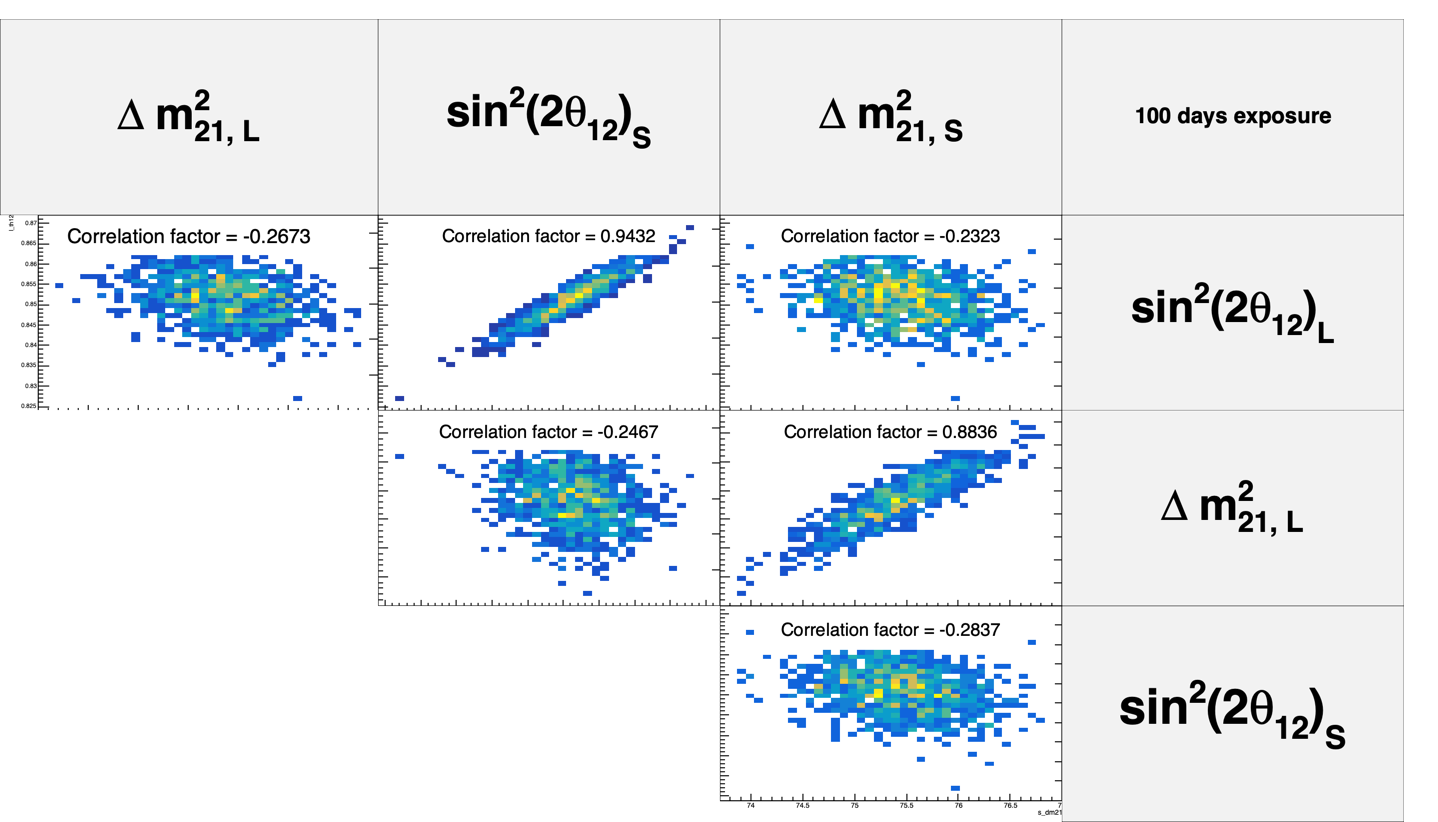
\includegraphics[height=6cm]{images/joint_fit/stat_tests/chi2_ind_corr_100d.png}
  \caption{Distribution and correlation between the best fit point of 1000 individual toys fit for 100 days exposure without supplementary QNL.}
  \label{fig:joint_fit:chi2_ind:corr:100d}
\end{figure}
\begin{figure}[ht]
  \centering
  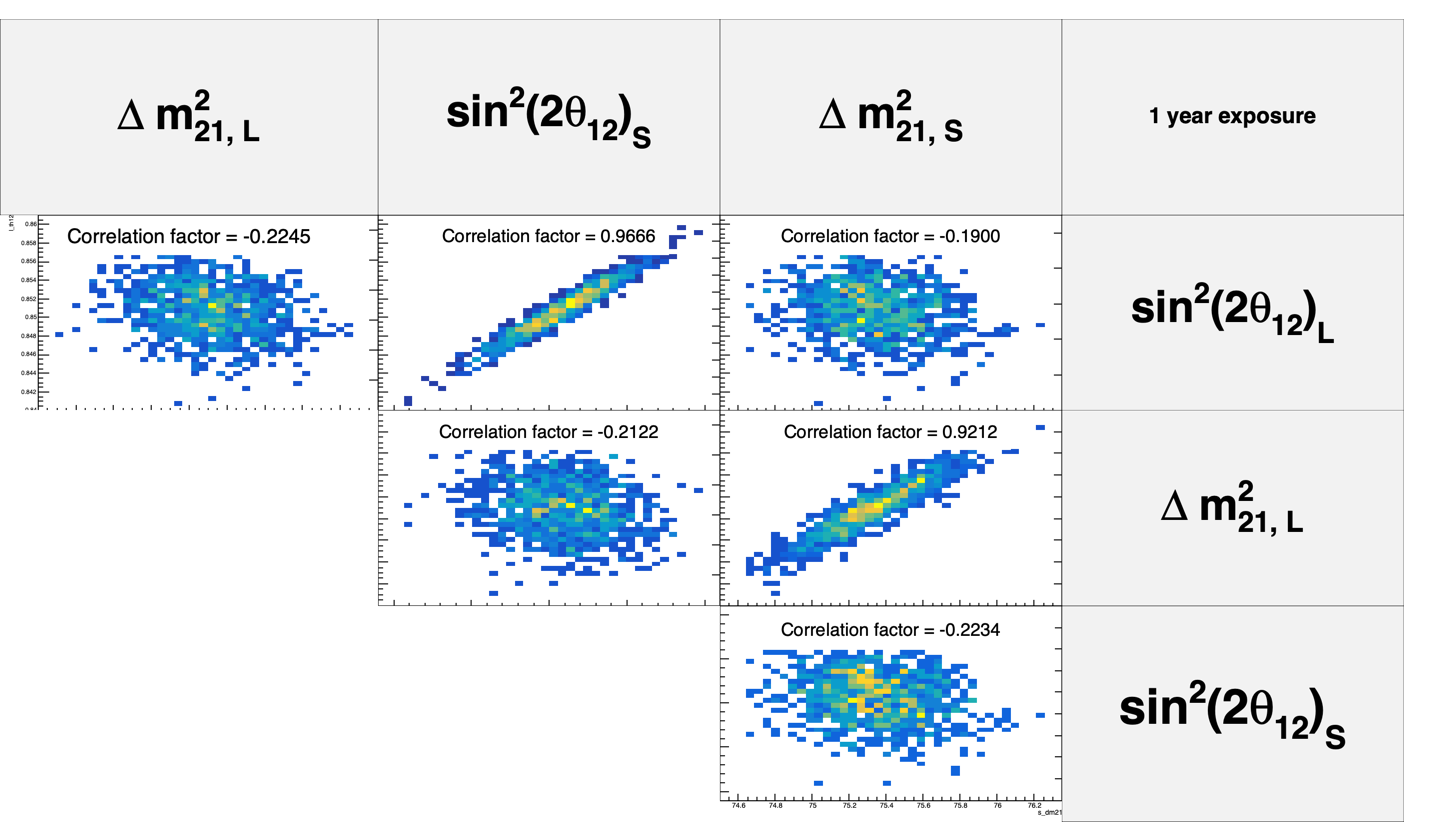
\includegraphics[height=6cm]{images/joint_fit/stat_tests/chi2_ind_corr_1y.png}
  \caption{Distribution and correlation between the best fit point of 1000 individual toys fit for 1 year exposure without supplementary QNL.}
  \label{fig:joint_fit:chi2_ind:corr:1y}
\end{figure}
\begin{figure}[ht]
  \centering
  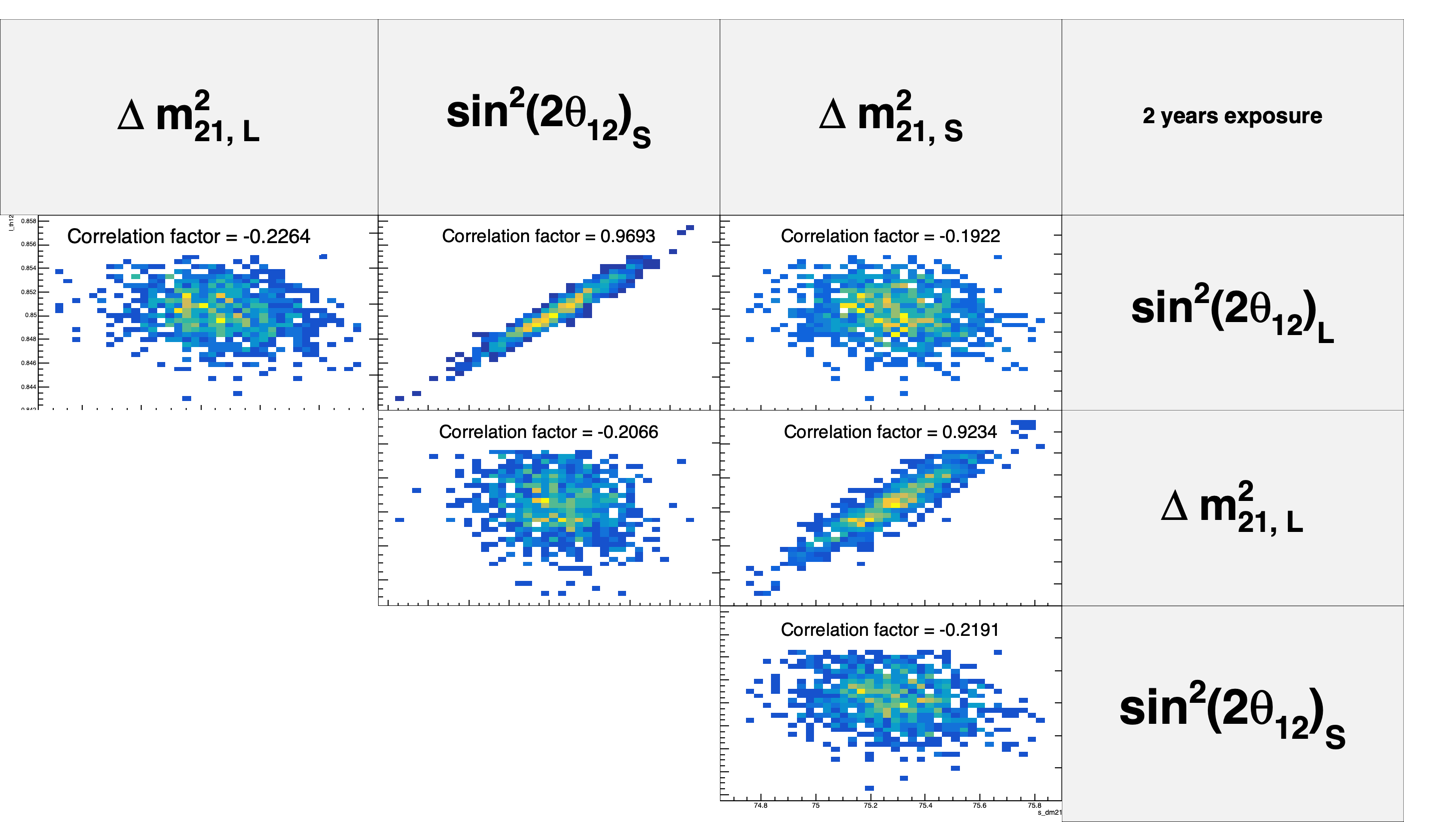
\includegraphics[height=6cm]{images/joint_fit/stat_tests/chi2_ind_corr_2y.png}
  \caption{Distribution and correlation between the best fit point of 1000 individual toys fit for 2 years exposure without supplementary QNL.}
  \label{fig:joint_fit:chi2_ind:corr:2y}
\end{figure}
\begin{figure}[ht]
  \centering
  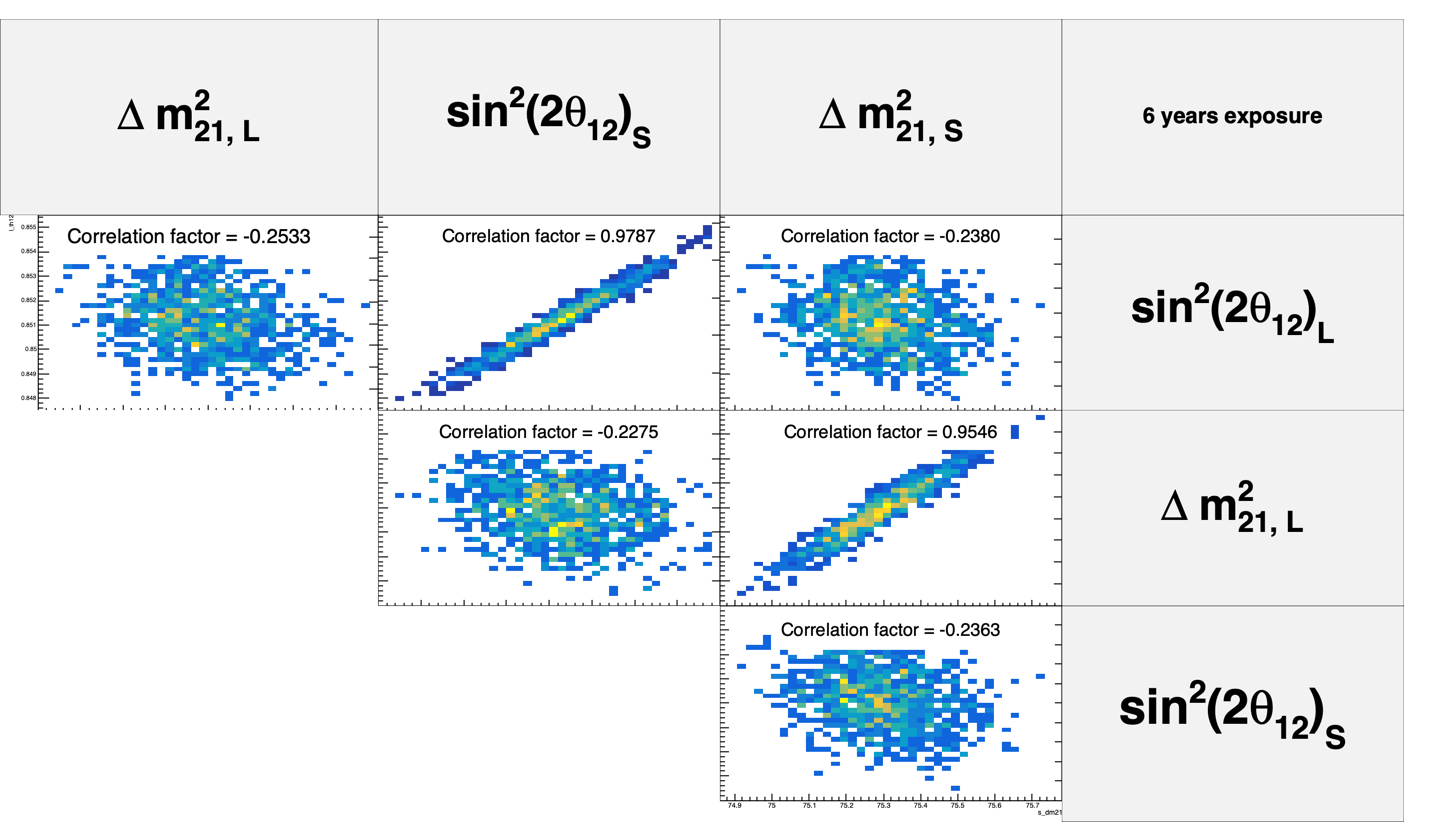
\includegraphics[height=6cm]{images/joint_fit/stat_tests/chi2_ind_corr_6y.png}
  \caption{Distribution and correlation between the best fit point of 1000 individual toys fit for 6 years exposure without supplementary QNL.}
  \label{fig:joint_fit:chi2_ind:corr:6y}
\end{figure}


We observe strong correlation between the reconstructed $\Delta m^2_{21}$ and $\sin^2(2\theta_{12})$ of both systems as presented in Table \ref{tab:joint_fit:ind_corr}, row one and two. As the relative statistical uncertainty decrease with exposure, the correlations grow ranging from 0.88 to 0.95 for $\Delta m^2_{21}$ and from 0.94 to 0.98 for $\sin^2(2\theta_{12})$. We observe between parameters of the same fit, a small anti-correlation of about -0.25, line 4 and 5 of Table \ref{tab:joint_fit:ind_corr}.

%This anti-correlation seems to be fluctuating over the exposure but, using the following formula, from \cite{gnambs_brief_2023}, as an estimator of the uncertainty over this coefficient
%\begin{equation}
%  \sigma(\rho) = \frac{1 - \rho^2}{\sqrt{N - 3}}
%\end{equation}
%where $\rho$ is correlation coefficient and $N$ the number of sample, the uncertainty on a -0.25 anti-correlation is 0.029. The measurement are compatible with a constant anti-correlation over the exposure.

\begin{table}
  \centering
  \begin{tabular}{l|c|c|c|c}
                                                                  & 100 days & 1 year & 2 years & 6 years \\
    \hline
    \hline
    Corr($\Delta m^2_{21,L}$,  $\Delta m^2_{21,S}$)               & 0.8836   & 0.9212 & 0.9234  & 0.9546 \\
    Corr($\sin^2(2\theta_{12})_{L}$, $\sin^2(2\theta_{12})_{S}$)  & 0.9432   & 0.9666 & 0.9693  & 0.9787 \\
    \hline
    Corr($\sin^2(2\theta_{12})_{L}$, $\Delta m^2_{21,L}$)         & -0.2673 & -0.2245 & -0.2264 & -0.2533 \\
    Corr($\sin^2(2\theta_{12})_{S}$, $\Delta m^2_{21,S}$)         & -0.2837 & -0.2234 & -0.2191 & -0.2363 \\
    \hline
    Corr($\sin^2(2\theta_{12})_{L}$, $\Delta m^2_{21,S}$)         & -0.2323 & -0.19   & -0.1922 & -0.2380 \\
    Corr($\sin^2(2\theta_{12})_{S}$, $\Delta m^2_{21,L}$)         & -0.2467 & -0.2122 & -0.2066 & -0.2275 \\
  \end{tabular}
  \caption{Correlations between the parameters BFP of the individual LPMT and SPMT fits for multiple exposures using 1000 toys.}
  \label{tab:joint_fit:ind_corr}
\end{table}

Because the parameters are heavily correlated between the LPMT and SPMT fit, and that $\Delta m^2_{21}$ and $\sin^2(2\theta_{12})$ are slightly anti-correlated in the same fit, the couples of different parameters from different fit, Corr($\sin^2(2\theta_{12})_{L}$, $\Delta m^2_{21,S}$) and Corr($\sin^2(2\theta_{12})_{S}$, $\Delta m^2_{21,L}$), are also anti-correlated.

The distributions $\chi^2_{ind}$ will be Shown in Section \ref{sec:joint_fit:results}.


\subsection{Direct comparison between the SPMT and LPMT spectra}
\label{sec:joint_fit:compar}

In the second test, we perform a bin-by-bin comparison of the LPMT and SPMT spectra without fitting any oscillation parameters.
Again, we use here a $\chi^2$-like statistics.
We do not expect the reference distribution (for $\alpha_{qnl}=0$) to be centered around the number of degree of freedom (i.e. the number of bins of each spectrum in our case) as should be distributed (if the spectra contain enough events in each bin to assume a gaussian behavior of the number of entries) the $\chi^2$ comparing 2 histograms when they are consistent with each other. Indeed, even in the absence of unexpected events, the LPMT and SPMT are quite different because of the very different reconstruction resolutions. We therefore need here again to establish this reference distributions with toys. And compare them later with the distributions obtained for the various tested values of $\alpha_{qnl}$.

Our test statistics is :
\begin{equation}
  \chi^2_{spe} = \bm{\Delta}_{spe}^T U^{-1} \bm{\Delta}_{spe}
\end{equation}
where
\begin{equation}
  \bm{\Delta}^{spe}_i = h_{L,i} - h_{S,i}
\end{equation}
and
\begin{equation}
  U = A V A^T
\end{equation}

Here, $i$ runs over the 410 bins of the individual spectra. Also, $h_{L,i}$ and $h_{S,i}$ are the contents of the $i$th bin of the LPMT and SPMT spectra respectively. We need to know the uncertainty on $\bm{\Delta}^{spe}_i$ and the correlations with $\bm{\Delta}^{spe}_j$ 's in other bins. We derive them from $V$, the $(820 \times 820)$ covariance matrix introduced at the beginning of this section, which can be seen as the covariance matrix of a 820-bin double spectrum juxtaposing the LPMT and SPMT spectra. We remind its determination will be presented in Section \ref{sec:joint_fit:cov_mat}. To obtain $U$ from $V$, we again apply the linear error propagation, with the transfer matrix :
\begin{equation}
  A_{ij} = \frac{\partial \bm{\Delta}^{spe}_i}{\partial h_j} = \frac{\partial(h_{L, i} - h_{S, i})}{\partial h_j}
\end{equation}
Thus, $A_{ij} = 1$ if $i = j$, and $A_{ij} = -1$ if $j$ is the SPMT bin corresponding to the $i$ LPMT bin.

We expect this statistics to have a certain power since $\chi^2_{spe}$ can be increased for 2 reasons in case of unexpected problem: first, the LPMT spectrum (if the LPMT is affected) will be distorted and become less consistent with the SPMT spectrum; second, the correlations between the LPMT and SPMT might also modified. Since $V$ present a peculiar correlation pattern (see Section \ref{sec:joint_fit:cov_mat}), a departure from this pattern also has some valuable impact on $\chi^2_{spe}$.

% Distributions of $\chi^2_spe$ in the reference case and for various values of alpha_qnl.

%   (b) Fits séparés
%     --- Fit individuel LPMT puis sPMT dans chaque toy.
%     --- Les N_toys résultats permettent d'établir la corrélation entre les param d'oscillations mesurés par les deux fits quand la génération ne suppose pas d'effets de reco imprévus.
%          => Description du test statistiques

%
%  (c) Fit joint
%
%     --- Un fit de chi2, ajustant aux deux spectres 2 pdf distinctes (par la modèle de reconstruction qu'elles supposent).
%
%     --- Les paramètres ajustés par le fit sont :  ...
%
%     --- Les paramètres fixes, ou contraints par un pull term : ...
%
%     --- Les pdf sont distinctes, mais les valeurs des paramètres d'oscillations sont communes aux deux fits.
%
%     --- Pour tenir compte d'un biais dû à un effet de reco imprévu, delta_th et delta_dm ajoutés à th12 et dm2_12 dans la pdf appliquée au spectre LPMT.
%
%     --- Nous avons là par défaut deux spectres de 410 bins, donc un spectre global de 820 bins. Nous effectuons un fit de chi2 : besoin d'une matrice de corrélation. Dans la plupart des fits joints entre spectres (comme lorsque l'on combine plusieurs expériences) la matrice de covariance statistique totale (celle entre les 820 bins dans notre cas) est diagonale car les différents spectres sont indépendants statistiquement. Là, nous avons pour défi de déterminer les corrélations statistiques entre les deux spectres. Expliqué en section xx.
%
%
%    => La statistique de test.


\subsection{Joint fit of the SPMT and LPMT spectra : $\chi^2_{H_0}-\chi^2_{H_1}$}
\label{sec:joint_fit:hypothesis}

This kind of fit has already been introduced in Section \ref{sec:juno:Fit}.
As a reminder, it involves the minimisation of
\begin{equation}
  \chi^2_{joint}=\left(\bm{T}(\bm{\theta},\bm{h}) - \bm{D} \right)^T V^{-1} \left(\bm{T}(\bm{\theta},\bm{h}) - \bm{D}  \right) + \ln(|V|)
\end{equation}
where $\bm{T}(\bm{\theta},\bm{h})$ is the predicted joint LPMT+SPMT spectrum and $\bm{D}$ the corresponding data vector. The matrix $V$ is the full $(820 \times 820)$ covariance matrix which incorporate both the statistical uncertainties and the bin-to-bin correlations between the LPMT and SPMT spectra.

In this fit, we include the usual oscillation parameters, $\sin^2 (2 \theta_{12})$, $\Delta m^2_{21}$, $\sin^2 (2\theta_{13})$ and $\Delta m^2_{31}$ along with two additional parameters, $\delta \sin^2(2\theta_{12})$ and $\delta \Delta m^2_{21}$ which allow for a potential discrepancy in the LPMT reconstruction or calibration.

Several remarks must be made here to better understand what we do precisely.
\begin{itemize}
  \item Given JUNO's lack of sensitivity to $\sin^2(2\theta_{13})$, this parameter is fixed in the fit to the PDG value (see table \ref{tab:joint_fit:pdg_value}). In most of JUNO's fit procedures (see Section \ref{sec:juno:Fit}), it's allowed to float during the minimisation, but is treated like a nuisance parameter, by adding a penalty term based on the PDG central value and uncertainty.


 \item The oscillation fit that we perform here does not really aim at the oscillation parameters in themselves, but is performed to detect a difference between the LPMT and SPMT spectra. JUNO is supposed to be very sensitive to $\Delta m^2_{31}$ via the LPMT spectrum. However, it has been shown by studies carried out at Subatech (and confirmed since then by other groups in the Collaboration), that up to 2 years of data taking, the presence of multiple minima in $\Delta m^2_{31}$ $\chi^2$ profile can make its determination delicate. Since $\Delta m^2_{31}$ is not the aim of our present study, we stabilize the fit by treating this parameter as a nuisance parameter, adding to $\chi^2_{joint}$ the following penalty term :
    \begin{equation}
      \chi^2_{\Delta m^2_{31}} = \frac{(\Delta m^2_{31}-\overline{\Delta m^2_{31}})^2}{\sigma^2_{\overline{\Delta m^2_{31}}}}
    \end{equation}
\end{itemize}
\hfill


We define two hypothesis. The hypothesis $H_0$ assumes that no unexpected effect is present, meaning that $\delta \sin^2(2\theta_{12}) = 0$ and $\delta \Delta m^2_{21} = 0$ , and the hypothesis $H_1$  where  $\delta \sin^2(2\theta_{12}) \neq 0$ and $\delta \Delta m^2_{21} \neq 0$ are needed to account for any potential calibration or reconstruction bias.
The test statistic is then defined as the difference between the minimized $\chi^2$ values under $H_0$ and $H_1$:
\begin{equation}
  \Delta \chi^2 = \chi^2_{joint,H0} - \chi^2_{joint, H1}
\end{equation}
where $\chi^2_{joint,H0}$ is the result of the minimisation when the fit assumed no unexpected effect (fixing $\delta \sin^2(2\theta_{12})$ and $\delta \Delta m^2_{21}$ to 0), while $\chi^2_{joint, H1}$ assumes a possible effect, letting this parameters free to float. A large value of $\Delta \chi^2$ would indicate a significant deviation from the null hypothesis (no discrepancy), suggesting the presence of an unexpected effect in the LPMT system.

Distributions of $\chi^2_{H_0}-\chi^2_{H_1}$ in the reference case and for various values of $\alpha_{qnl}$ will be produced and studied in Section \ref{sec:joint_fit:results}.

The idea behind this joint fit is that by letting the oscillation parameters and $\delta \sin^2(2\theta_{12})$ and $\delta \Delta m^2_{21}$ free to float, converging potentially to arbitrary, wrong values in the case of oscillation parameters, we add some flexibility to fully exploit the difference introduced by unexpected effects between the reference spectra and correlations.

There were other reasons to develop this joint fit. The main one was that it required an update of our software framework so it's able to perform joint fit. It was not fully ready for that. This feature will be very useful when the Subatech team will include the TAO spectrum (via a joint fit) in the oscillation studies it will perform.

\subsection{Joint fit of the SPMT and LPMT spectra : distribution of $\delta \sin^2(2\theta_{12})$ and $\delta \Delta m^2_{21}$}
\label{sec:joint_fit:delta_distrib}

The last test statistics we will study might be complementary to $ \Delta \chi^2 = \chi^2_{joint,H0} - \chi^2_{joint, H1} $.

These test statistics are simply the fitted values of $\delta \sin^2(2\theta_{12})$ and $\delta \Delta m^2_{21}$. In the reference case, when no unexpected reconstruction problem
is present, we expect them to be distributed in an approximate gaussian way, centered on 0. When QNL effect will be included, they will tend to converge to higher values, to compensate the bias introduced on the fitted $\sin^2(2\theta_{12})$ and $\Delta m^2_{21}$ due to the distortion of the LPMT spectra and of the correlations between the LPMT and SPMT spectra.

Again, these distributions will be studied in Section \ref{sec:joint_fit:results}.

\begin{table}
  \centering
  \begin{tabular}{c|c|c|c}
    $\sin^2(2\theta_{12})$    & $\Delta m^2_{21}$                       & $\Delta m^2_{31}$      & $\sin^2(2\theta_{13})$ \\
    \hline
    $0.851^{+0.020}_{-0.018}$ & $7.53 \pm 0.18 \times 10^{-5}$ eV$^2$   & $2.5283 \pm 0.034 \times 10^{-3}$ eV$^2$  & $0.0.8523 \pm 0.00268$
  \end{tabular}
  \caption{Nominal PDG2020 value \cite{particle_data_group_review_2020}. All value are reported assuming Normal Ordering.}
  \label{tab:joint_fit:pdg_value}
\end{table}

%
%   (d) Les suppositions
%
%       --- Nous travaillons en traitant que des erreurs statistiques. Cela se justifie pour un travail exploratoire dans la mesure où une grande partie des effets syst sont totalement corrélés (ceux qui affectent le spectre vrai des neutrinos et des bruits de fond, voir table XX -- systèmatiques du papier Subpercent. )
%
%        --- L'essentiel de nos résultats supposent les effets de détection décorrélés entre LPMT et sPMT. Ils sont par ailleurs introduits de manière simpliste (simple tirage gaussien supposant une résolution gaussienne ne dépendant pas de la position de l'intéraction dans le détecteur --conforme à la publi Subpercent et à la dernière publi NMO). Ce choix se justifie pour un travail exploratoire par la nécessité de produire un grand nombre de toys malgré une puissance de calcul limitée. Un premier raffinement de cette approche tenant compte des corrélations entre les deux reconstructions est présenté en fin de chapitre. Il s'appuie sur la simulation complète du détecteur, et sur notre algo CNN de reco sPMT, le seul disponible à ce jour.
%
%        ---- La QNL est introduite de manière un peu simpliste pour l'instant (appliquée à nouveau juste en fonction de l'énergie de l'IBD). Rappeler que tu as tout de même établi une correspondance (alpha_qnl vs. gamma_qnl) en commençant à faire le boulot qu'il faudrait faire : l'appliquer au niveau des PMT (ce qui tient compte des effets de position de l'intéraction).

\subsection{Limitations}
\label{sec:joint_fit:approach:lim}

\subsubsection{QNL in backgrounds}

The JUNO commons inputs provides background spectra that already have been smeared by the LPMT resolution. Because the resolution depends on $E_{vis}$ (Eq. \ref{eq:joint_fit:abc}), to apply supplementary QNL we would need to de-convolute the LPMT resolution, apply the supplementary QNL then re-smear the spectra. This deconvolution is no trivial. Thus we ignore the background when produced distorted spectra.

This should not affect too much the power of our statistical tools, as the backgrounds are common to both spectra and should not have any effect on the statistical covariance matrix.

\subsubsection{Systematics}
It would be more rigorous to also include systematic uncertainties. However, in the present state of our fit framework, it would require the computation (often empirical, via the generation of thousands of toy samples) of $(820 \times 820)$ covariance matrices, which was judge too time consuming with respect to the time we could devote to this chapter.

Moreover, it seems reasonable to think that the sensibilities evaluated with only statistical uncertainties would not be changed much by a full treatment. Indeed, all the systematic uncertainties affect the true visible energy spectrum, before reconstruction. This spectrum is a common input to both the LPMT and SPMT reconstructions. Therefore, observed differences between the oscillation parameters measured by one or the other system should not be due to these systematics effects, and remain of the same order as if these effects were absent.

\subsubsection{Correlation between LPMT and SPMT reconstruction}

Most of our results assume uncorrelated reconstruction uncertainties between the SPMT and LPMT systems. In practice, once the $E^{vis}$ of a toy event is generated (see Section \ref{sec:joint_fit:framework:ibd-gen}), we simulate the SPMT and LPMT reconstruction by adding a $\delta E^{rec}_{SPMT}$ and a $\delta E^{rec}_{LPMT}$.

The two latter increments are chosen randomly on Gaussian distribution. These two drawings are carried out independently. In reality, the reconstruction of $E^{vis}$ is about proportional to the number of PE, therefore to the number of scintillation photons produced in the scintillator. Both the LPMT and SPMT reconstruction depend on the stochastic variation of this number event to event. Their results therefore vary in a correlated way. The correlation is kept low since it is shuffled by another source of variability, namely the sampling of photons : the SPMT indeed reconstruct only a few dozen PEs when more than 10000 photons are emitted.

This correlation is higher when the interaction takes place close to the sphere's surface (ie close to some of the PMTS), the non-uniformity effect is correlated between the two systems. To account for it, when should ideal produce the simulated samples necessary to our studies by using the full simulation. However, it would be far too CPU intensive. The impact of neglecting this correlation will be discussed in Section \ref{sec:joint_fit:cov_mat}.

\subsubsection{Realistic QNL}

The way we implement the QNL effect in toy samples is also simplified. The size of the QNL effect in a PMT depends on the number of photons hitting it, therefore on the position of the interaction. When generating toy events, we apply QNL event-wise, only as a function of the value of $E^{vis}$ (Eq. \ref{eq:joint_fit:alpha_yang}). As explained in Section \ref{sec:joint_fit:qnl}, the full simulation has been used to find the average $\alpha_{qnl}$ for a given $\gamma_{qnl}$ which is considered sufficient for this exploration.

Again, replacing toy samples with samples generated with the full simulation would yield more accurate results, but is prohibitive in terms of calculation time. For future studies, sophisticated solutions to this problem  will have to be found, but are out of the scope of this thesis.


\section{Fit software}
\label{sec:joint_fit:framework}

In this section, I describe the fit framework that was used in this study. The AveNu$_e$ framework is the adaptation to JUNO of one of the frameworks, partly developed at Subatech, used by the Double Chooz \cite{double_chooz_collaboration_double_2022} experiment. It is composed of two parts: the AveNu$_e$ Generators and the AveNu$_e$ Fitting Package. The Generators are a set of standalone macros, the Fitting Package is an C++ package, using the RooFit library.


Both parts of the package are interfaced with what we call the JUNO inputs.
These inputs comprise all the ingredients to build a $\bm{T}(\bm{\theta}, \bm{\eta})$ prediction, among which :

\begin{itemize}
  \item Reactor antineutrino spectra for each isotope as predicted by Mueller \cite{mueller_improved_2011-1}.
  \item The isotopes mean releases energy.
  \item Reactors´s thermal powers and fission fractions.
  \item Various corrections to account for the contributions from the Non Equilibrium Regime and the Spent nuclear fuel.
  \item A correction obtained by comparing these spectrum prediction in the case of the Daya Bay experiment with actual Daya Baya data \cite{daya_bay_collaboration_measurement_2016}.
  \item The IBD differential cross section as function of the antineutrino energy.
  \item The assumed values of the oscillation and nuisance parameters at the start of the fit or for sensitivity studies.
  \item Parameters describing the non linearity of the photon emission as a function of the deposited energy.
  \item Energy reconstruction parameters (see equation \ref{eq:joint_fit:abc} and Figure \ref{fig:joint_fit:system_resolution}).
  \item The selected IBD and background expected yields per day, and the background spectra, all obtained from JUNO's full simulation and studies to design the selection.
  \item Uncertainties on all these quantities for the computation of covariance matrices.
\end{itemize}
\hfill

We describe in the next section the role of each part of the framework.


\subsection{AveNu$_e$ Standalone Generators}

The main macro here is the ``IBD generator'' macro. It is used to :

\begin{itemize}
  \item Compute $\bm{T}_{no~osc}(\bm{\eta})$ (unoscillated theoretical spectra) predictions. It is done by toy generating a spectrum. In order to not be affected by statistical fluctuations, it generates 100 times more statistics that JUNO's expected yield after 6 years. It is provided in the form of a TTree. These predictions concern an non oscillated spectrum.

  \item Toy samples simulated data sets. It is essentially used to simulate data spectra altered by QNL effects (see below).

  \item The above productions are input to the Fitting Package, or to other macros from Standalone Generators, which compute the covariance matrices necessary to the Fitting Package. Some of the covariance matrices are computed from the $\bm{T}$'s, using linear error propagation, some other are empirical calculations based on sets of toy samples generated with varying parameters. This is also the case for one of the versions of the computation of the $V_{stat}$ covariance matrix of the LPMT+SPMT double spectrum (see Section \ref{sec:joint_fit:cov_mat}).
\end{itemize}



\subsection{AveNu$_e$ Fitting Package}
\label{sec:joint_fit:avenue_fit}

Its role is to perform fits to a single data samples, of to a set of toy samples. In practice :

\begin{itemize}
  \item It loads TTrees containing the data to fit as well as the $\bm{T}_{no~osc}(\bm{\eta})$ predictions, and create local objects representing the data spectrum and the pdf. For that purpose, $\bm{T}_{no~osc}(\bm{\eta})$ are changed into predictions $\bm{T}(\bm{\theta},\bm{\eta})$ for the oscillated spectrum by weighting events in the TTree according to the oscillation probability.
  \item It loads the necessary covariance matrices.
  \item It creates from this a $\chi^2$ object. The Pearson, Neyman, CNP and Pearson V versions are available

  \item It is interfaced with Minuit via RooFit classes to perform the minimisation. At each step, $\bm{T}(\bm{\theta},\bm{\eta})$ are re-weighted by the oscillation probability corresponding to the current value of the floating oscillation parameters.
\end{itemize}
\hfill

Three kinds of data can be fitted with this Package : real data, Asimov simulated data and toy data.

When real data will be available at JUNO, we expect that the result of the IBD selection will be made available by the collaborations via TTrees.

The principles of Asimov fits were described in Section \ref{sec:juno:Fit:asimov}. In practice, our Fit Package fill the local object representing the data spectrum with $\bm{T}(\bm{\theta}, \bm{\eta})$, assuming some values for the oscillation parameters.

The toy data samples can have two origins. Some are produced by the IBD generator macro of the AveNu$_e$ Generators. This is the case of the toy samples that we produce with QNL effects. It is also possible to generate toys directly with the Fitting Package. In that case, toy data spectra are produced by generating random fluctuations around
each the values of $\bm{T}(\bm{\theta}, \bm{\eta})$.These fluctuations must be the reflect of both statistical and systematic uncertainties. Fluctuations between bins $i$ and $j$ can be correlated. Such correlations are common in the case of systematic uncertainties. In general, they are 0 for the statistical uncertainties. In our case, as already explained earlier (see for instance the Sections where the test statistics are described), bins from the SPMT part of the LPMT+SPMT spectrum are correlated to bins of the LPMT part even for the statistical part.

To generate correlated fluctuation we use, through Choleski decomposition, the covariance matrices. This way to generate toy is faster. We use it in this work in the reference case (no QNL). In the case where QNL effects are simulated, the corresponding statistical covariance matrix is not known, we therefore resort to the IBD generator.


% IV) Le framework de fit.
% ---------------------------------------
%
% ... Description plus ou moins détaillée suivant qu'il a, ou non, déjà été décrit ailleurs...
%
%   (a) Introduction avec rapide overview
%
%
%   (b) La partie standalone : IBD-gen
\subsection{Details of the IBD generator}
\label{sec:joint_fit:framework:ibd-gen}

The IBD generator is a standalone generator used to produce oscillated and non oscillated spectra as the one seen by the JUNO experiment. It is at the core of the fitting framework as it's used to generate $\bm{T}(\bm{\theta}, \bm{\eta})$, the toy data and spectra to compute the covariances matrix.

With thus have a flexible macro with options allow to enable or disable effects such as non-uniformity and non-linearity. It take as an argument the number of events to generate $N_{evt}$. Optionally, we generate an effective number of events $N$ by drawing in a Poisson distribution of mean $N_{evt}$.

Then for each event we:
\begin{enumerate}
  \item Choose randomly, following the reactor power fraction, the source reactor of the neutrino.
  \item Generate a random interaction position in the detector following a uniform distribution over the detector volume.
  \item Draw a random neutrino energy $E_{\nu}$ from the expected neutrino emission spectrum of every reactor. This spectrum is computed by:
    \begin{enumerate}
      \item Computing the power spectrum of each isotopes $^{235}$U, $^{238}$U, $^{239}$Pu, $^{241}$Pu using the Huber-Mueller model \cite{huber_determination_2011, mueller_improved_2011}.
      \item Summing the contribution of each isotopes following the respective fission fraction [0.58, 0.07, 0.30, 0.05] as reported in \cite{ma_improved_2013}.
      \item The power of each reactor is then adjusted by their distances from the detector, the detector efficiency and their mean duty cycle (11 of 12 month).
      \item The total spectrum is then finally adjusted by taking into account the correction of the Day Bay bump \cite{daya_bay_collaboration_measurement_2016}, adjustment due to spent nuclear fuel and due to the non-equilibrium.
    \end{enumerate}
  \item \textit{(Optional)} Compute the survival probability due to oscillation at nominal oscillation parameters value. If the neutrino does not survive, the event is rejected and the algorithm restart from step (1).
  \item Compute the emitted positron energy $E_{pos}$ from the mass difference. If the neutrino does not have enough energy reject the event and start from step (1).
  \item Compute the deposited energy $E_{dep}$ by incrementing $E_{pos}$ by 511 keV to account for the positron annihilation. We do not consider cases where some of the energy leak outside of the detector (positron or annihilation gammas escaping the CD).
  \item Correct the deposited energy with the expected event-wise non-linearity from \cite{juno_collaboration_calibration_2021} to obtain the visible energy $E_{vis}$.
  \item \textit{(Optional)} Add a custom non-linearity as described in Section \ref{sec:joint_fit:qnl}. This non linearity is characterized by $\alpha_{qnl}$ to obtain $E_{\alpha}$.
  \item Finally, using the expected resolution of the LPMT and SPMT systems,  provided in the JUNO common inputs, we draw from a gaussian characterized by those resolution the reconstructed energy $E_{rec}$ or $E_{lpmt}$ and $E_{spmt}$ for each systems. The resolutions are provided as ABC parameters using
    \begin{equation}
      \label{eq:joint_fit:abc}
      \frac{\sigma E_{vis}}{E_{vis}} = \sqrt{\bigg(\frac{A}{\sqrt{E_{vis}}}\bigg)^2 + B^2 + \bigg(\frac{C}{E_{vis}}\bigg)^2}
    \end{equation}
    where A is the term driven by the Poisson statistics of the total number of detected photoelectrons, C is dominated by the PMT dark noise, and B is dominated by the detector’s spatial non-uniformity. The relative and absolute resolutions of the LPMT and SPMT systems are illustrated in Figure \ref{fig:joint_fit:system_resolution}.
\end{enumerate}

The events are stored as n-tuples and are not yet binned at the end of the generator.

\begin{figure}[ht]
  \centering
  \begin{subfigure}[t]{0.48\linewidth}
    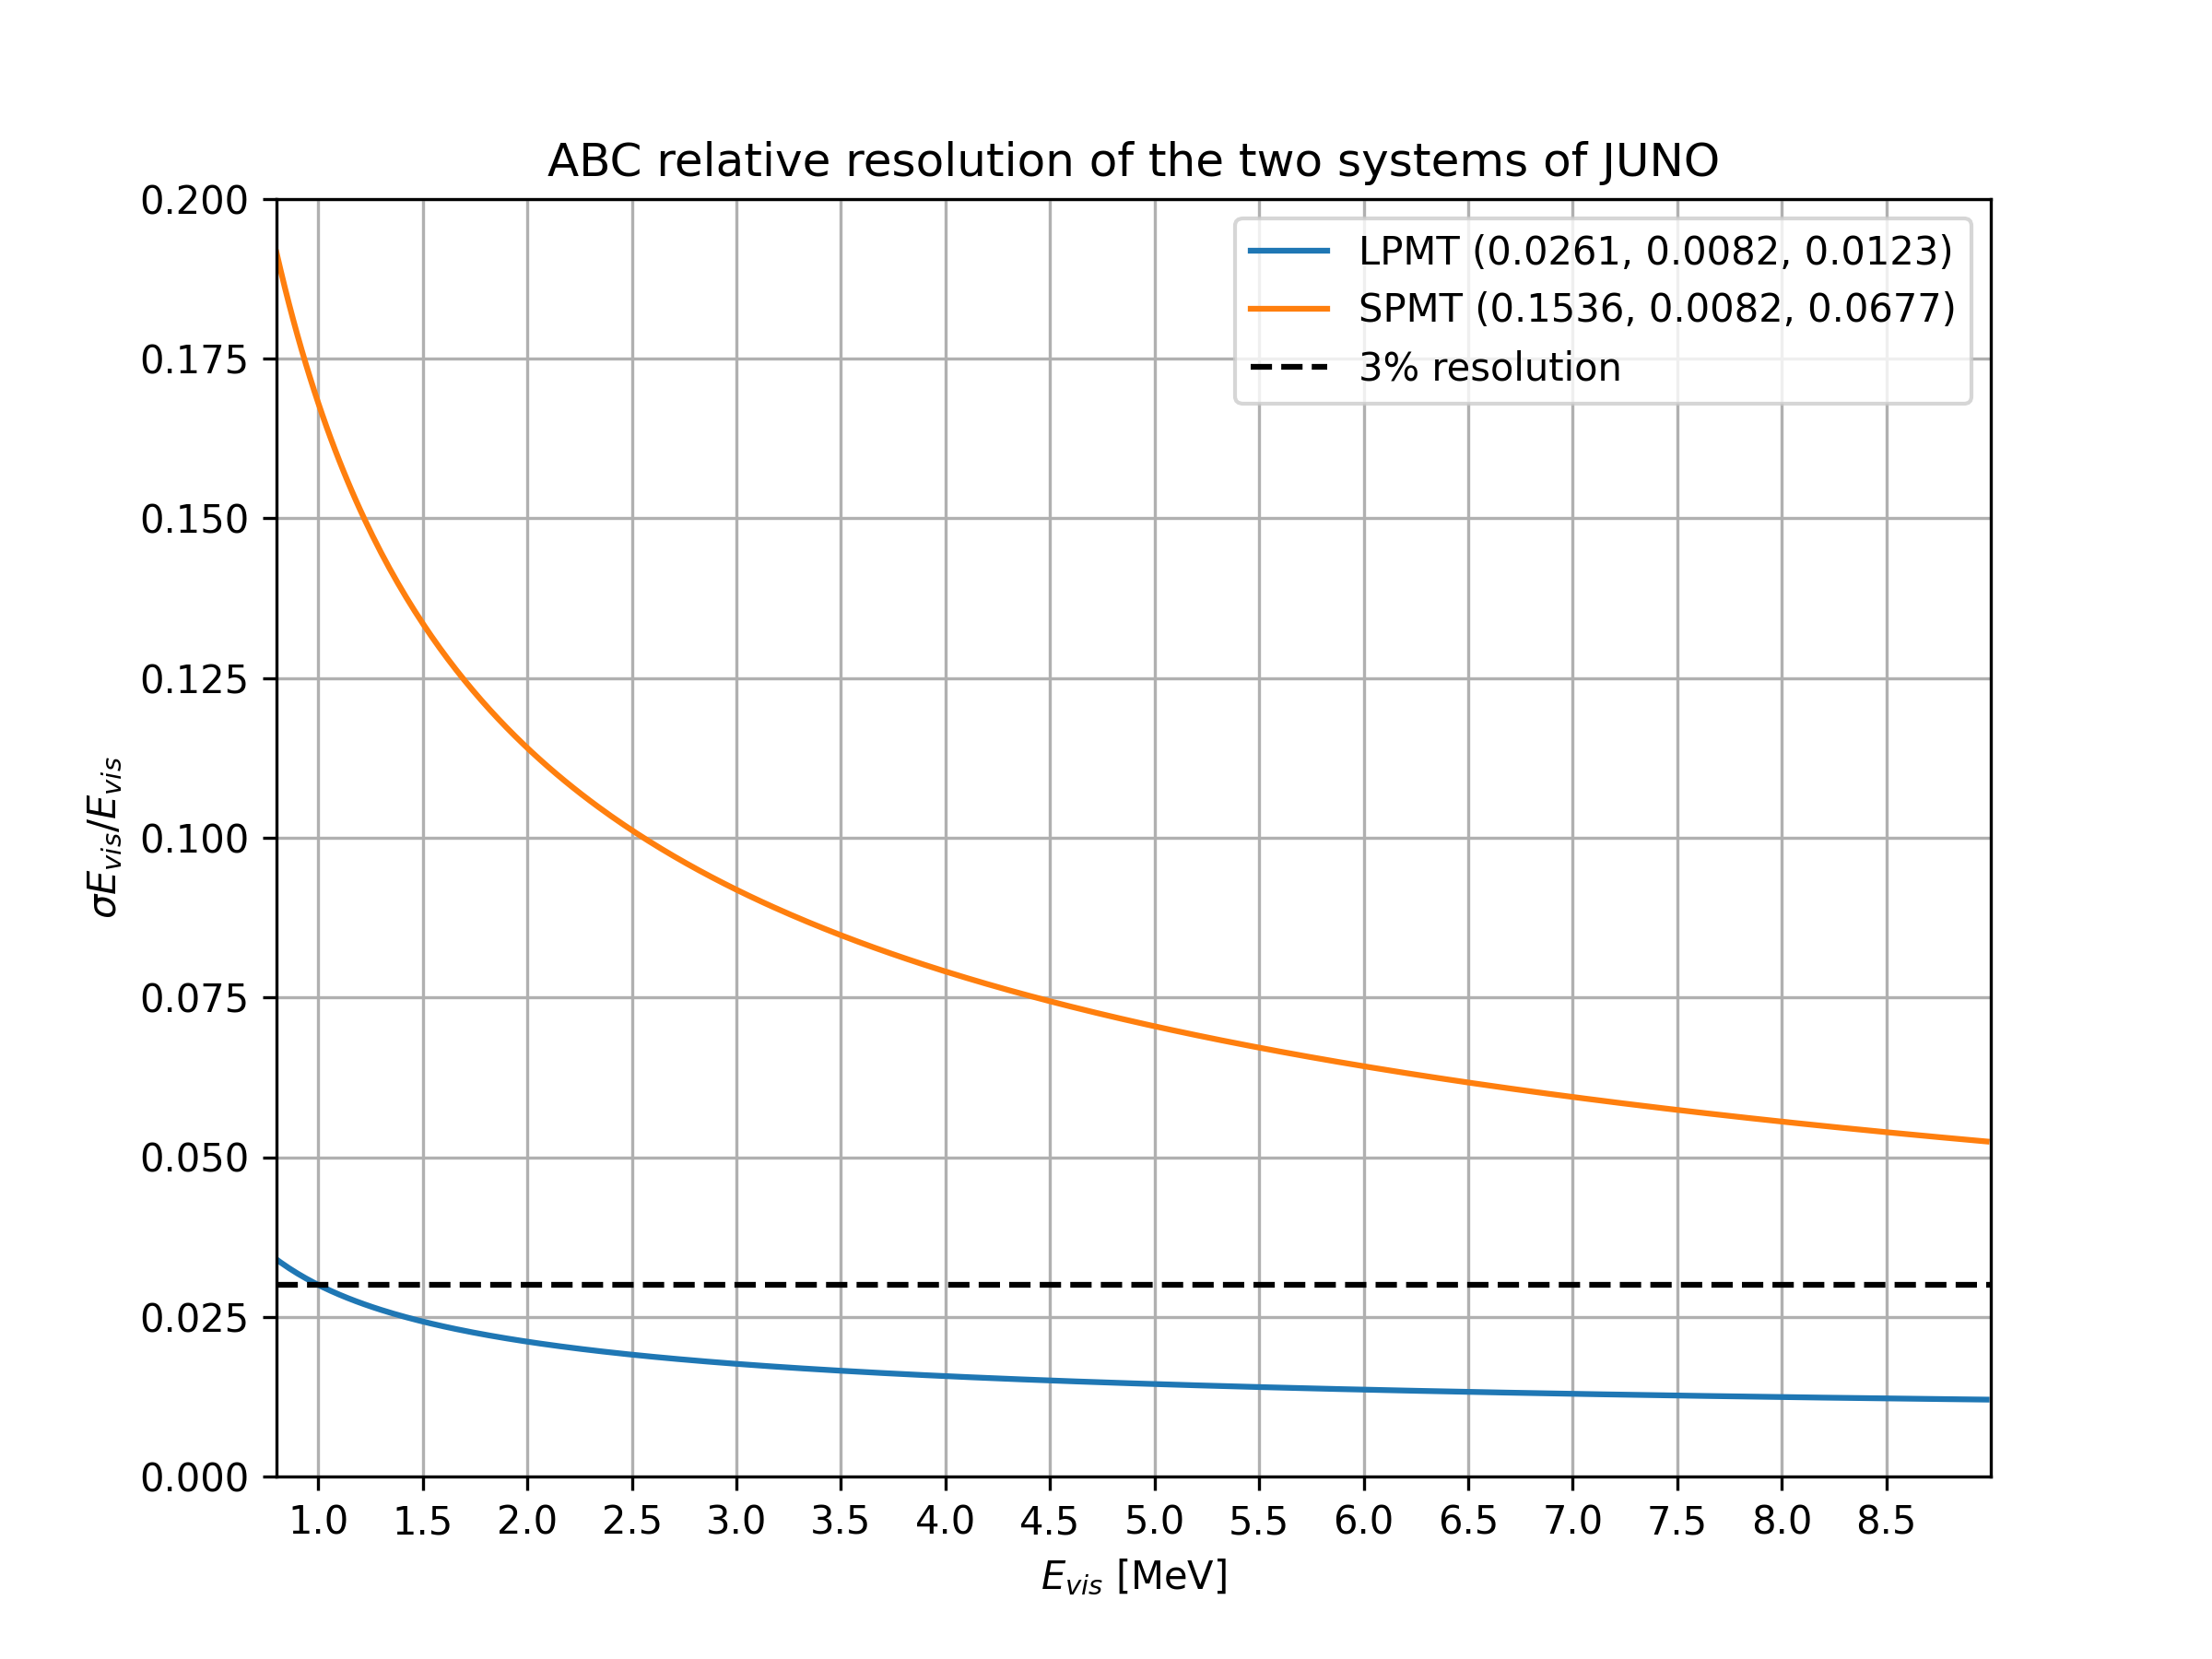
\includegraphics[width=\linewidth]{scripts/plots/relative_resolution.png}
  \end{subfigure}
  \hfill
  \begin{subfigure}[t]{0.48\linewidth}
    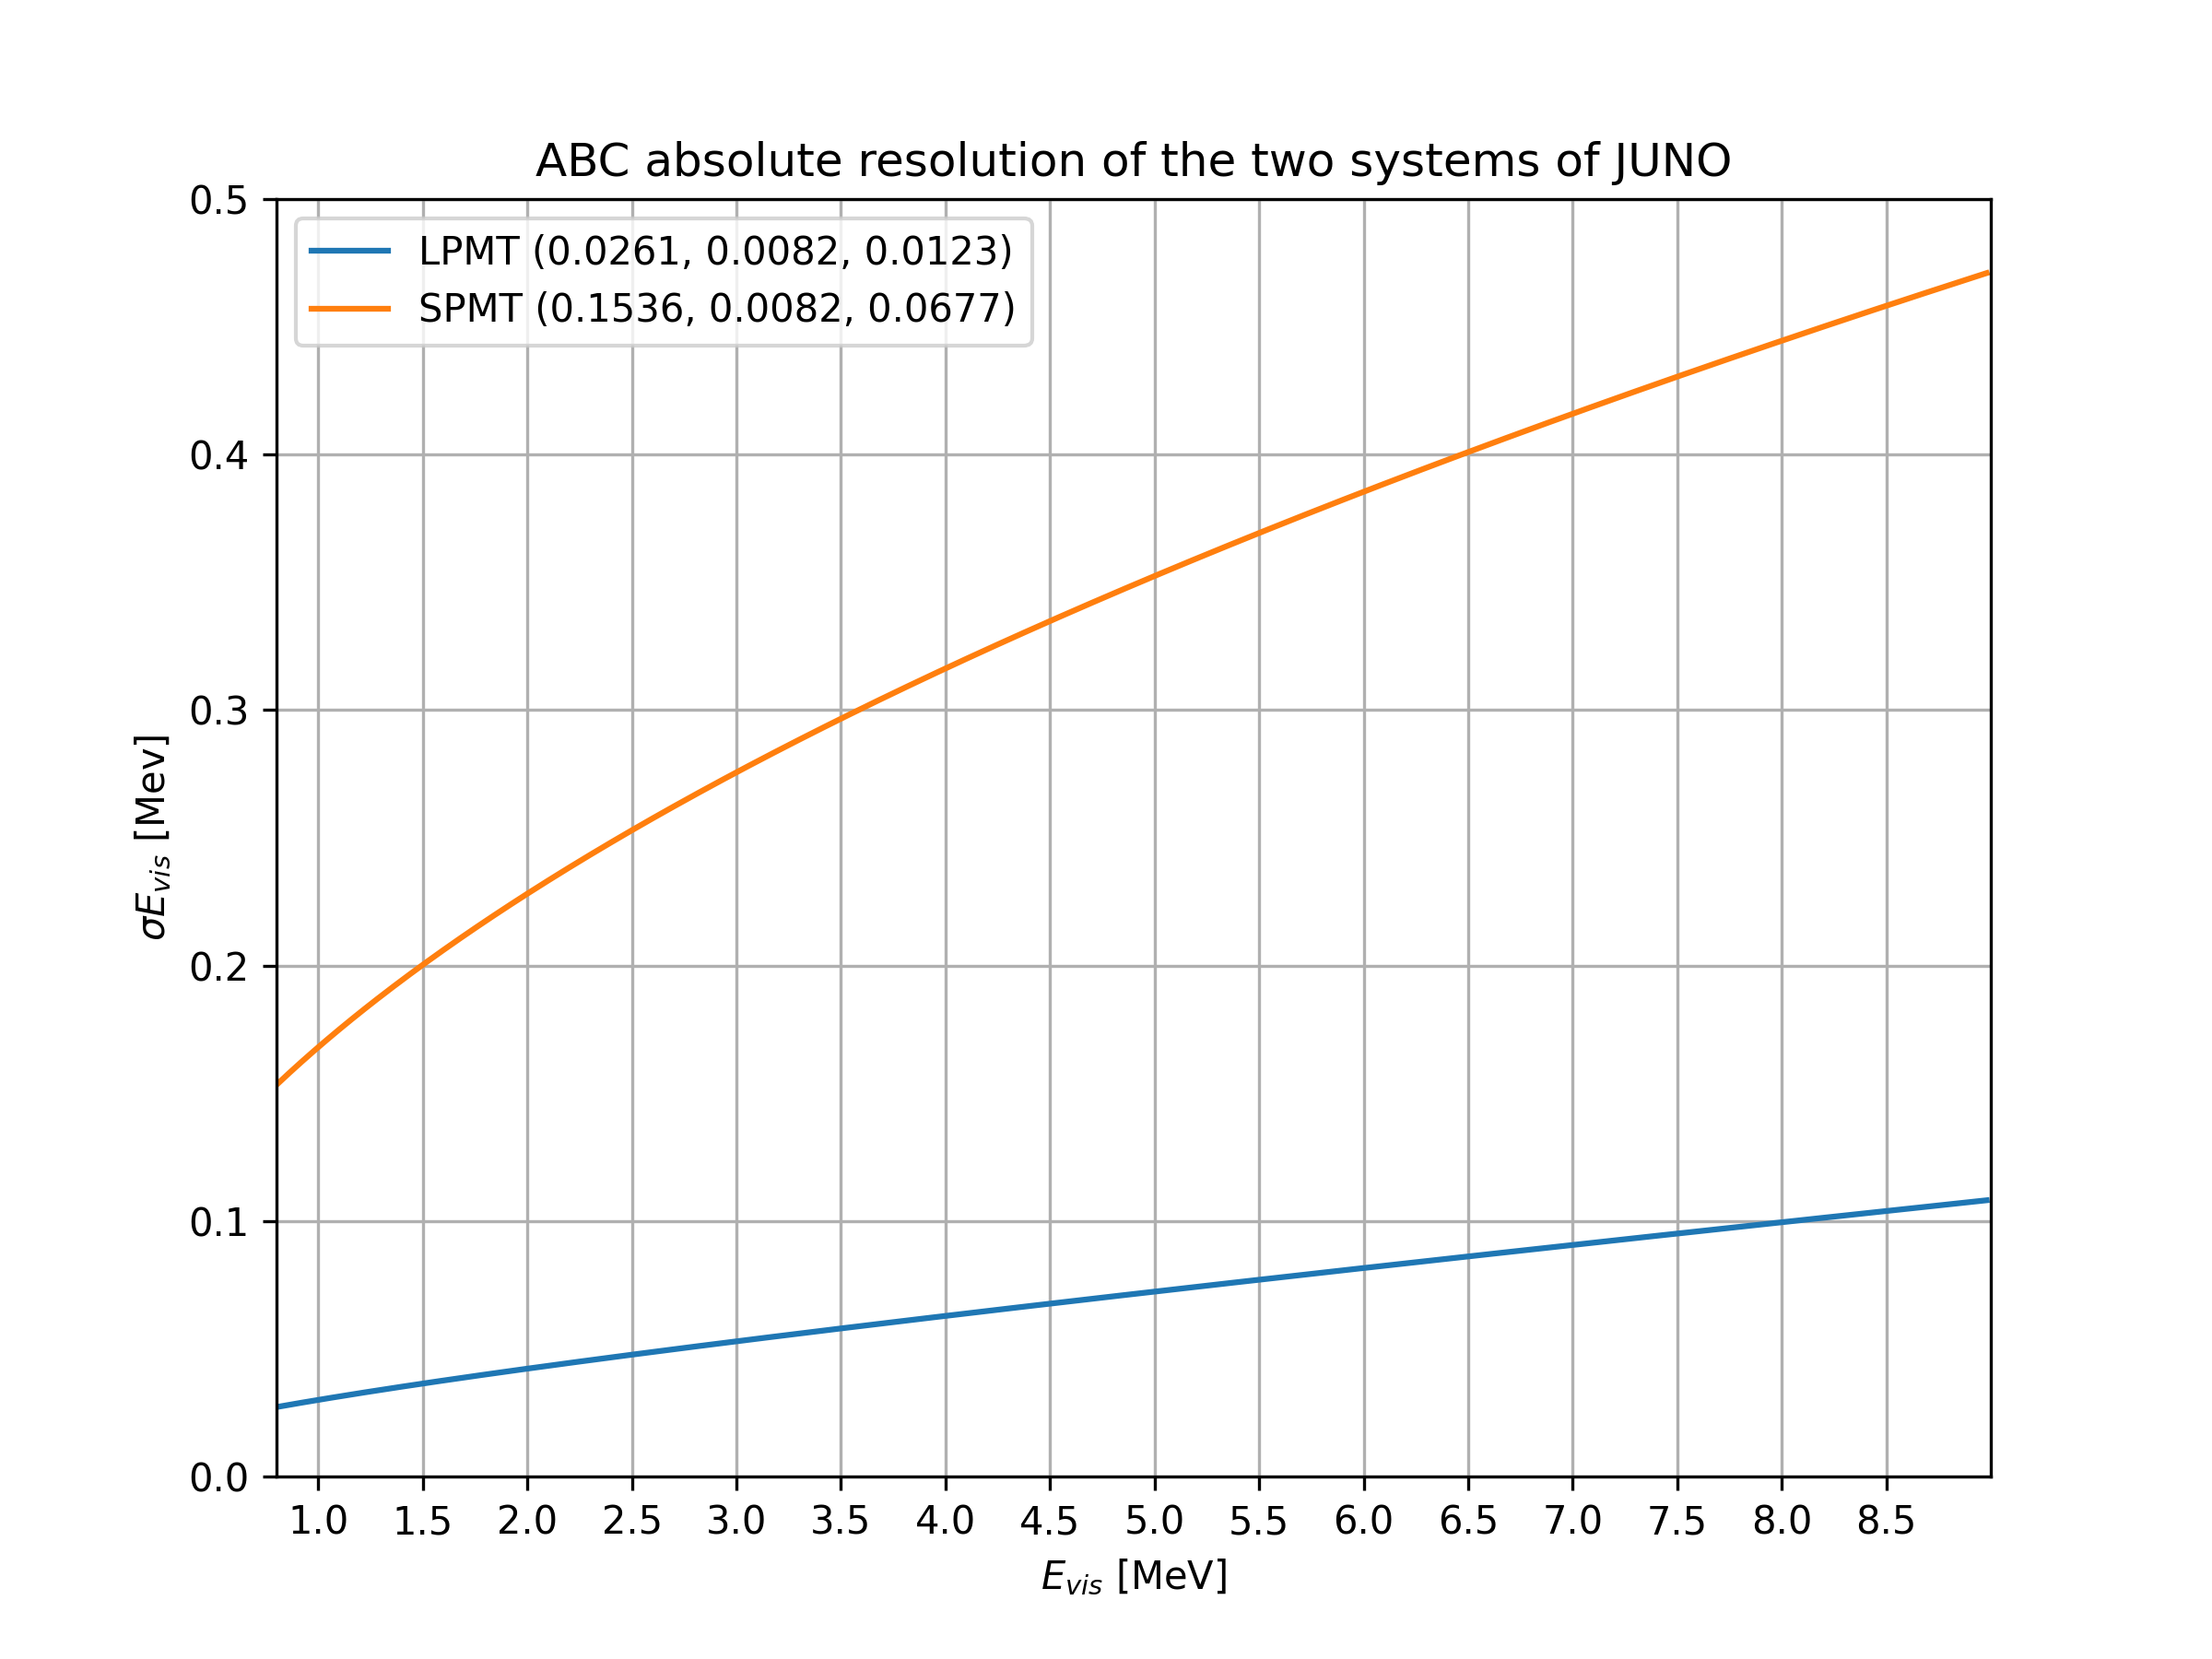
\includegraphics[width=\linewidth]{scripts/plots/absolute_resolution.png}
  \end{subfigure}
  \caption{Relative (\textbf{On the left}) and absolute (\textbf{On the right}) resolutions of the LPMT and SPMT systems used in this study. The number in parenthesis are the parameter $A$, $B$ and $C$ respectively for each systems.}
  \label{fig:joint_fit:system_resolution}
\end{figure}

%
%   (c) Le framework de fit intégré.

% V) Tes développements techniques.
% -----------------------------------------------------------
%
%   (a) Pour générer les divers toys et pdf dont on a besoin, avec ou sans QNL.
%      --- Bien préciser les deux façons de générer des toys : dans IBDgen, ou dans le fmwk intégré, à partir de la matrice de corr et de Choleski.
%
%    (b)  Pour que le framework intégré soit capable de faire un fit joint.
%
% À ce stade, le lecteur doit comprendre comment tout est fait en pratique, et réaliser la quantité de travail technique que cela a demandé.
\section{Technical challenges and development}
\label{sec:joint_fit:tech}

The fit framework Avenue was already partially developed with multispectra fitting in mind but a lot technical development was necessary to allow for a joint fit. This required a lot of work and constitute a good part of my total effort on this study. I remind that these development will be useful beyond this thesis and this subject. As already mentioned earlier, at some point, we should perform simultaneous fits of the JUNO and TAO spectra. It's also a potential starting  point for combined analyses with other experiments, like long baseline experiments.

The first step was to migrate the framework from ROOT5 (last release in March 2018) to ROOT6 (v6.26.06 released in July 2022) to ensure compatibility with the data coming from the JUNO collaboration, and benefiting of the improvement and corrections that came with ROOT6. This allow us to upgrade the C++ standard from C++11 to C++17. A substantial effort has been done to modernize the code, generalizing the functions and methods via templating to help readability and using smart pointer to prevent possible memory leaks.

The Avenue framework had to be adapted, notably on the chi-square calculation and spectrum generation to correctly take into account the correlation between the SPMT and LPMT spectra. The delta joint fit requiring two more parameters over a spectrum twice as large as before with LPMT takes much more time, around 15h for 6 years exposure, than the single LPMT fit. Thus the framework and the fit macro had to be updated for distributed computing. Notably the aggregation of fit results can now be done in a single file instead of managing a file per fit. In case of numerous toy, the hard drive access time could lead to long analysis time.

While the IBD generator was already able to generate LPMT and SPMT spectrum, it was not designed for generating correlated spectrum. As detailed in Section \ref{sec:joint_fit:framework:ibd-gen}, up to the reconstruction effect, the two spectrum need to share the same generation else the two spectrum would be decorrelated and it would be like we would run two different experiment.
% VI) Résultats
% ----------------------
%
%    (a) Validations techniques.
%
%        i- Les test Asimov sans QNL que nous avions faits, pour valider que le fit joint est OK techniquement (joint vs. Moyenne pondérée des fit individuels) et notamment que la matrice a été mise correctement.
%
%        ii- Tous les autres que je n'ai plus en tête.



\section{Covariance matrix}
\label{sec:joint_fit:cov_mat}

The covariance matrix between the LPMT and SPMT spectra is at the heart of this study as it was already mentioned in Section \ref{sec:joint_fit:approach}. In this section we discuss the different approaches taken to estimate it.
We remind that in this work, we consider only statistical effects and let to future works the task to include systematic uncertainties. We thus evaluate in this section the $(820\times820)$ statistical covariance matrix $V$ of the LMPT+SPMT spectrum.

As already explained in previous Sections \ref{sec:joint_fit:approach:lim} and \ref{sec:joint_fit:framework:ibd-gen}, we assume, in most of what follows, that the effect of the energy reconstruction resolution is independent between the LPMT system and the SPMT system, although this is an approximation. We therefore also briefly study the correlations between the two reconstructions.

\subsection{Analytical method}

The first method discussed is the analytical method where we propagate the resolution of the LPMT and SPMT spectra over a non-smeared spectrum. Following the approach used in the IBD generation in Section \ref{sec:joint_fit:framework:ibd-gen}, we consider the system resolution $\sigma(E)$ to be only dependent in energy. We do not consider the position of the event.

% The first step is to compute the statistical uncertainty of the input spectrum while taking into account the smearing, considering no uncertainty on the smearing.
Using the formalism of section \textit{39.2.5 Propagation of errors} of PDG2020 \cite{particle_data_group_review_2020} and considering an extended spectrum of 820 bins following the binning scheme introduced in \ref{sec:juno:fit:subatech}, the first 410 for the LPMT and the last 410 for the SPMT, we consider
\begin{itemize}
  \item $\bm{h} = (h_0, ..., h_n)$ Is the n-dimensional vector (n=820) containing the number of entries in each bin of the LPMT+SPMT true $E^{vis}$ spectrum.
  \item $\bm{\zeta}(\bm{h}) = (\zeta_0(\bm{h}), ..., \zeta_n(\bm{h}))$ is the n dimensional vector containing the reconstructed $E^{vis}$ LPMT+SPMT spectrum.
\end{itemize}

Since, like in most sensitivities studies, resolution is simulated via a gaussian smearing, $\bm{\zeta}$ can be expressed this way :
\begin{equation}
  \label{eq:joint_fit:cov_ana:eta}
  \zeta_i  = \sum_{j=0}^n G(j, \sigma(E_j))(i) \cdot h_j
\end{equation}
where $G(j, \sigma(E_j))(i)$ is the smearing function defined as
\begin{equation}
  \label{eq:joint_fit:smear}
  G(j, \sigma(E_j))(i) = \int_{\lfloor E_i\rfloor}^{\lceil E_i \rceil} \frac{1}{\sigma(E_j)\sqrt{2\pi}} e^{-\frac{(E_j-E)^2}{2\sigma(E_j)^2}} \dd{E}
\end{equation}
where $E_j$ is the mean energy in the bin $j$ and $\lfloor E_i\rfloor$ and $\lceil E_i \rceil$ are the lower and higher energy bound of the $j$th bin respectively.

According to \ref{eq:joint_fit:smear}, to evaluate $V$, the matrix describing the uncertainties on $\zeta_i$'s  and the correlations between them, one has to consider uncertainties both on $h_j$ 's and on $G(j,\sigma(E_j))(i)$'s. We use linear error propagation and split this problem in two steps : $V = V_{inputs} + V_{rec} $. The first matrix accounts for the uncertainties on the inputs from the true $E^{vis}$ spectrum ( $h_i$'s ), while the second concerns the uncertainties due to $G(j,\sigma(E_j))(i)'$s.

To evaluate $V_{inputs}$, we use $V_{inputs} = AUA^T$ where $U$ is the covariance matrix of the LPMT+SPMT true $E^{vis}$ spectrum.
Since before reconstruction the LPMT and SPMT spectra are the same, this LPMT+SPMT is the juxtaposition of two 410-bin identical spectra. Moreover we are interested only in statistical uncertainties. Therefore, $U$ has the form :

\begin{equation}
  U = \begin{cases}
    \sqrt{h_ih_j}& \text{if } i = j \text { or } |i - j| = 410 \\
    0& \text{otherwise}
  \end{cases}
\end{equation}

The condition $|i - j| = 410$ express the fact that one $h_i$ of the LPMT part of the spectrum is naturally 100\% correlated with the corresponding binin the SPMT spectrum.

We can then construct the transfer matrix $A$ as
\begin{equation}
  A_{ij} = \frac{\partial\zeta_i}{\partial h_j} = G(j, \sigma(E_j))(i)
\end{equation}
and then compute the first part of our covariance matrix
\begin{equation}
  V_{inputs} = A U A^T
\end{equation}

Now we need to consider the uncertainty on the steaming from the resolution, ie to evaluate $V_rec$. It can be done considering no uncertainty on the true $E_{vis}$ spectrum.
The quantity $G(j,u) \equiv G(j,\sigma(E_j))(i)$ is the predicted probability for an event initially in bin $j$ of the true Evis spectrum to be reconstructed in bin $i$. In pratice, the migration between these bins is a random process. Reconstructed many times the same event would not lead each time the same migrations. We need here to determine this variability. We consider that with 410 bins, migrations vary independently whatever $i$ and $j$.

This allows to consider $V_{rec}$ as diagonal, thus we only need $\sigma G(j,i)$.
We can derive this term from two equation:
\begin{itemize}
  \item The term $G(j, i) \cdot h_j$ represent the number of event smeared from the bin $j$ that end up in the bin $i$. This is a number, we thus assume poissonian statistic so that $\sigma[G(j, i) \cdot h_j] = \sqrt{G(i, j) \cdot h_j}$.
  \item Using basic error propagation we can say that $\sigma^2[G(i, j) \cdot h_j] = h_j^2 \sigma^2G(j, i) + G(j, i)^2 \sigma^2 h_j$.
\end{itemize}
Equating the above equations, and remembering that $\sigma h_j=\sqrt{h_j}$ since $h_j$ is also a number of events :
\begin{align}
  G(j, i) h_j &= \sigma^2[G(j, i)h_j] =h_j^2 \sigma^2G(j, i) + G(j, i)^2 h_j \\
  \Rrightarrow \sigma^2 G(j, i) &= \frac{G(j, i) h_j - G(j, i)^2 h_j}{h_j^2} \\
                                &= \frac{(1 - G(j, i))G(j, i)}{h_j}
\end{align}

By summing the two covariance matrix $V_{inputs}$ and $V_rec$, we can extract a correlation matrix presented in Figure \ref{fig:joint_fit:th_cor_mat}.
Typically, a bin in the SPMT part of the reconstructed spectrum is correlated up to a few percents to the corresponding bin in the LPMT spectrum and its neighbour. This might seem a small correlation. However, its concerns all bins. The global impact is therefore high. As an illustration, as seen in Section \ref{sec:joint_fit:approach:comp}, the correlation between the value of $\sin^2(2 \theta_{12})$ measured with the LPMT spectrum and that measured with the SPMT spectrum are correlated at more than 95\%.

The correlation between the SPMT and LPMT spectra is greater at the start of the spectrum. This is expected since the absolute resolution is smaller in this region. For instance, at 1.5 MeV,  the reconstruction by the SPMT re-distribute events with a sigma of more that 0.20 MeV. At 6 MeV, this is about twice more. Since the resolution reduces the initial correlations (true Evis spectra are share by both LPMT and SPMT, correlations are 100\%), we therefore expect higher remaining correlations where the absolute resolution is smaller.

\begin{figure}[ht]
  \centering
  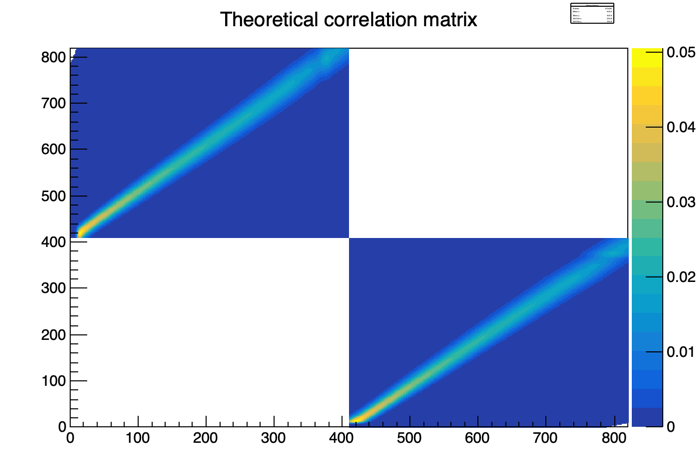
\includegraphics[height=6cm]{images/joint_fit/theoretical_corr.png}
  \caption{Theoretical correlation matrix between the LPMT spectrum (bins 0-409) ans the SPMT spectrum (410-819). The diagonal has been set to 0 (it was 1) for readability purpose.}
  \label{fig:joint_fit:th_cor_mat}
\end{figure}

\subsection{Empirical method}
\label{sec:joint_fit:cov_mat:emp}

The second method is the emprical way where we generate toys and just compute the empirical correlation between the bin contents.
\begin{equation}
  \mathrm{Corr}(h_i, h_j) = \frac{\mathbb{E}[h_i h_j] - \mathbb{E}[h_i] \mathbb{E}[h_j]}{\sigma h_i \sigma h_j}
\end{equation}

We thus generate $10^7$ event using the IBD generator presented in Section \ref{sec:joint_fit:framework:ibd-gen}, then produce spectra from this finite set of events, meaning we must choose a number $N$ of toy each composed of $M$ event in order to have the best estimate.

It can be shown that empirical correlations are more precise when one maximises the number of samples, even at the price to have few events per sample. This effect is illustrated in Figure \ref{fig:joint_fit:empirical_cor}.

%Due to the nature of our estimator, the estimated correlation coefficient is subject to statistical fluctuation as any estimator. There is no definite formula to compute the standard deviation of the correlation coefficient as suggested in this study \cite{gnambs_brief_2023} but all cited formula depend solely on the number of samples, in our case the number of toy $N$, and the correlation coefficient. This indicate that maximizing the number of toy is the right decision, even if each toy posses only one sole event.
%
%To study this rather counter intuitive observation (How can a spectrum with only one event can be representative of the experiment ?), I present in Figure \ref{fig:joint_fit:empirical_cor} the upper left corner of the estimated correlation matrix for different configurations of N and M in the limit of $10^7$ total event. Wee see in Figure \ref{fig:joint_fit:empirical_cor:small} that if the toy number $N$ is too low, the statistical noise make the correlation pattern almost completely disappear, in Figure \ref{fig:joint_fit:empirical_cor:medium} we see clearly the same correlation patter as in the theoretical matrix in Figure \ref{fig:joint_fit:th_cor_mat}.
%On the final matrix in Figure \ref{fig:joint_fit:empirical_cor:cheff_kiss} the pattern is clearly visible, but we see a shade of anti-correlation around the spectrum that was not present in the theoretical correlation matrix.

\begin{figure}[ht]
  \begin{subfigure}[t]{0.33\linewidth}
    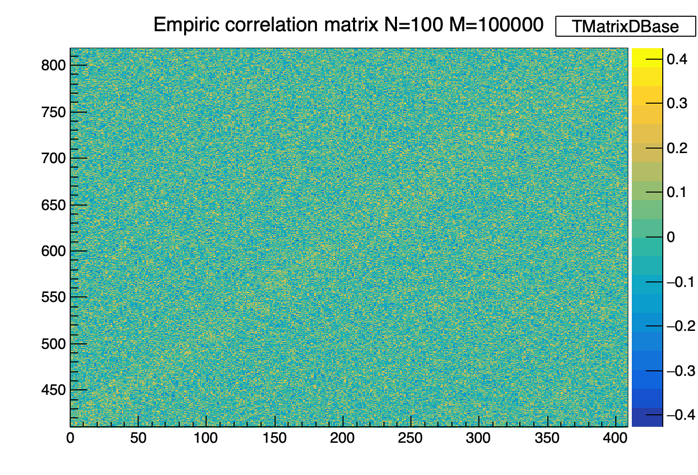
\includegraphics[width=\linewidth]{images/joint_fit/estimated_corr_N_100_M_100000.png}
    \caption{}
    \label{fig:joint_fit:empirical_cor:small}
  \end{subfigure}
  \begin{subfigure}[t]{0.33\linewidth}
    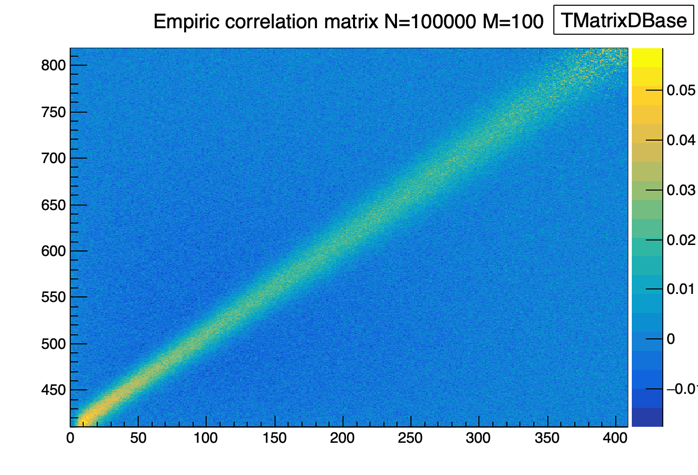
\includegraphics[width=\linewidth]{images/joint_fit/estimated_corr_N_100000_M_100.png}
    \caption{}
    \label{fig:joint_fit:empirical_cor:medium}
  \end{subfigure}
  \begin{subfigure}[t]{0.33\linewidth}
    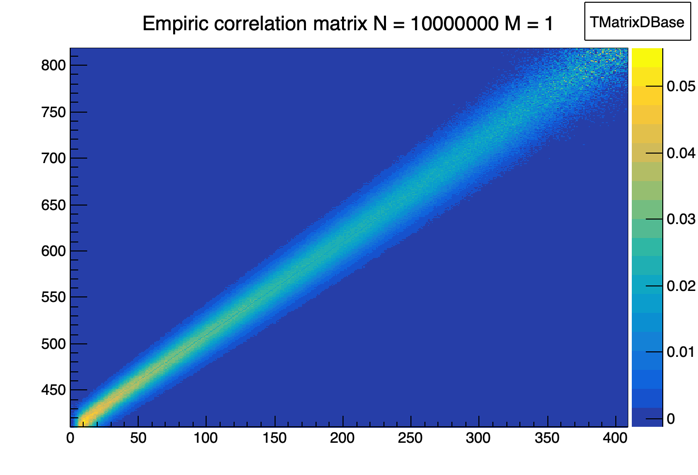
\includegraphics[width=\linewidth]{images/joint_fit/estimated_corr_N_10000000_M_1.png}
    \caption{}
    \label{fig:joint_fit:empirical_cor:cheff_kiss}
  \end{subfigure}
  \caption{Upper left corner of the estimated correlation matrix between the LPMT and SPMT spectrum for different configuration of $N$ toy with different number of $M$ events per toy. We observe that the statistical uncertainty, the noise effect, diminish with the number of toy considered.}
  \label{fig:joint_fit:empirical_cor}
\end{figure}


The relative difference between the element of the theoretical matrix of Figure \ref{fig:joint_fit:th_cor_mat} and the empiric correlation matrix in Figure \ref{fig:joint_fit:empirical_cor:cheff_kiss} is presented in Figure \ref{fig:joint_fit:th_em_diff}.
Typically,  correlations coefficient differ by 20\% of their value. We have verified that differences larger than this are confined in the very low or high end of the energy spectrum, which carry no sensitivity to the solar oscillation parameters we aim at. Therefore, for the statistical tests presented in this chapter we assume the correlations present in the theoretical version of $V$. This should account for the effect of correlations well enough.

\begin{figure}[ht]
  \centering
  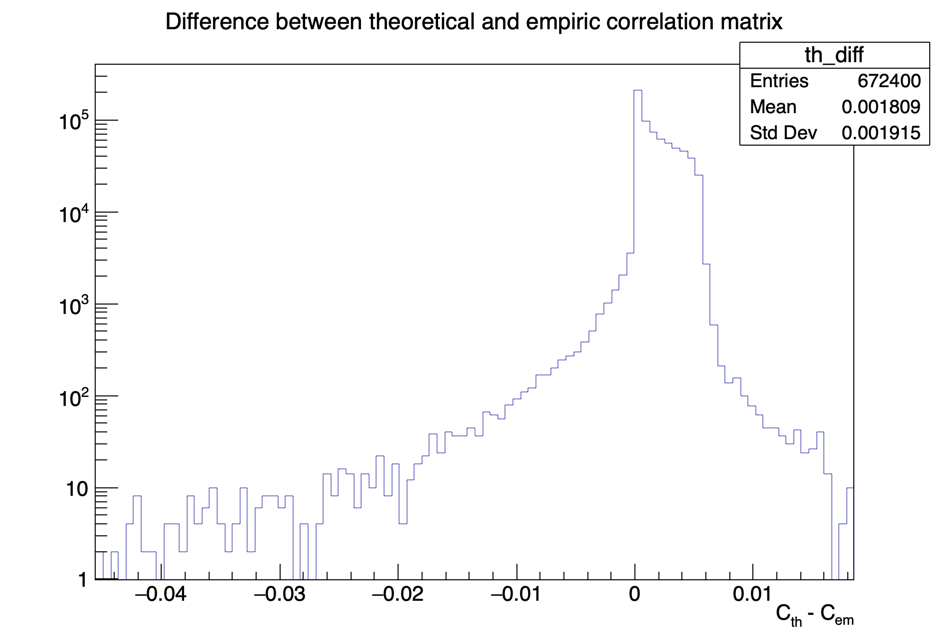
\includegraphics[height=6cm]{images/joint_fit/th_em_corr_diff.png}
  \caption{Relative difference between the element of the theoretical and empiric correlation matrix}
  \label{fig:joint_fit:th_em_diff}
\end{figure}

We chose to do so for practical reasons. Indeed, for the $\chi^2$ computation and the Choleski decomposition (see Section \ref{sec:joint_fit:avenue_fit}) the matrix must be invertible and positive definite. The statistical uncertainty on the coefficient of the empiric matrix can prevent that, leading to complications.

\section{Technical Validation}
\label{sec:joint_fit:validation}

\subsubsection{Standard Independent Joint Fit}


We have already explained in Sections \ref{sec:joint_fit:approach} and \ref{sec:joint_fit:cov_mat} that a correlation exist between the SPMT and LPMT spectra, and is accounted for in the LPMT+SPMT joint fit by the $V$ covariance matrix, which determination is described in the previous section.

We can, however, perform a test where we ignore these correlations, setting to 0 all off-diagonal elements of $V$. In this case, we implicitly assume that our data contains more information, and therefore expect the uncertainties on $\Delta m^2_{21}$ and $\sin^2(2 \theta_{12})$ to be smaller that those obtained with individual fits to the LPMT and SPMT spectra. Assuming a gaussian behavior of the number of entries per bin, these uncertainties should be close to the weighted average of the uncertainties with the individual fits :
\begin{equation}
  \label{eq:joint_fit:weighted_average}
  \frac{1}{\sigma^2_{Weighted}} = \frac{1}{\sigma^2_{LPMT}} + \frac{1}{\sigma^2_{SPMT}}
\end{equation}

These tests are performed using an Asimov sample. Indeed, if it was done via a toy study, then generating correlated toy spectra and fitting them assuming a diagonal $V$ matrix would have let to biases, regardless of the quality of the technical implementation. Asimov spectra, on the other hand, are generated with no fluctuations. They are supposed to return fitted values of $\Delta m^2_{21}$ and $\sin^2(2 \theta_{12})$ exactly equal to the values assumed during the generation. This is, together with the comparison with $\sigma_{weight}$, a strong test of the technical implementation.

Note that we fix here the $\delta m^2_{21}$ and $\delta \sin^2(2 \theta_{12})$ parameters to 0. Also, we assume 6 years of data taking, and the absence of unexpected instrumental effects (no supplementary QNL). A notable difference with the fit configuration used later in this chapter (and presented in Section \ref{sec:joint_fit:approach}) is that we do not treat $\Delta m^2_{31}$ as a nuisance parameter. It is free to float.


\begin{table}[ht]
  \begin{footnotesize}
  \centering
  \begin{tabular}{l | c | c | c | c | c | c }
                                    & $\sigma(\Delta m^2_{21})$ [eV$^2$]  & $\sigma(\delta \Delta m^2_{21})$ [eV$^2$]& $\sigma(\sin^2(2\theta_{12}))$  & $\sigma(\delta \sin^2(2\theta_{12}))$ & $\sigma(\Delta m^2_{31})$ [eV$^2$] & $\chi^2$ \\
                                    \hline
  LPMT                                 & 1.29 $\times 10^{-07}$   &                          & 1.33 $\times 10^{-03}$   &               & 4.39 $\times 10^{-06}$   & 3.23 $\times 10^{-18}$ \\
  SPMT                                 & 1.38 $\times 10^{-07}$   &                          & 1.38 $\times 10^{-03}$   &               &                          & 2.87 $\times 10^{-18}$ \\
  Indep Standard joint                 & 9.48 $\times 10^{-08}$   &                          & 9.86 $\times 10^{-04}$   &               & 4.39 $\times 10^{-06}$   & 6.10 $\times 10^{-18}$ \\
  Standard joint                       & 1.29 $\times 10^{-07}$   &                          & 1.18 $\times 10^{-03}$   &               & 4.39 $\times 10^{-06}$   & 3.38 $\times 10^{-18}$ \\
  Weighted                             & 9.46 $\times 10^{-08}$   &                          & 9.63 $\times 10^{-04}$   &               &               & \\
  \hline
  Delta joint                          & 1.35 $\times 10^{-07}$   & 3.43 $\times 10^{-08}$   & 1.38 $\times 10^{-03}$   & 1.46 $\times 10^{-04}$   & 4.39 $\times 10^{-06}$   & 3.38 $\times 10^{-18}$ \\
  Indep Delta joint                    & 1.38 $\times 10^{-07}$   & 1.89 $\times 10^{-07}$   & 1.38 $\times 10^{-03}$   & 1.87 $\times 10^{-03}$   & 4.39 $\times 10^{-06}$   & 6.10 $\times 10^{-18}$ \\
  \hline
  \end{tabular}
  \end{footnotesize}
  \caption{Uncertainties on each parameters reported by Minuit on Asimov studies. LPMT and SPMT rows are the results on the individual fit on each spectra. The Weighted row correspond to the weighted average uncertainties between the LPMT and SPMT fits following Eq. \ref{eq:joint_fit:weighted_average}. The Indep Standard joint row is the result of the joint LPMT+SPMT fit but the off-diagonal terms are set to 0. The Indep Standard joint and Standard joint fits both are LPMT+SPMT fit but the parameters $\delta m^2_{21}$ and $\delta \sin^2(2 \theta_{12})$ are fixed to 0. The Delta joint and Indep Delta joint are LPMT+SPMT fit with $\delta m^2_{21}$ and $\delta \sin^2(2 \theta_{12})$, difference being that in the Indep version, the off-diagonal terms of the covariance matrix are set to 0.}
  \label{tab:joint_fit:asimov_results}

\end{table}


The results are reported in Table \ref{tab:joint_fit:asimov_results}. All those test are ran considering statistics error only, 6 years exposure with all backgrounds, $\sin^2(2 \theta_{13})$ fixed to its nominal value. For the SPMT individual fit $\Delta m^2_{31}$ is fixed at its nominal value as the SPMT system is not sensitive to this parameter. We use here the simple Pearson $\chi^2$. Indeed, as explained above, an Asimov fit is supposed to find exactly the values of the parameters assumed for the generation of the spectrum, which implies a very low Pearson $\chi^2$ (0 modulo
numerical effects). This is also a strong indication that the technical implementation is correct. If we had used the usual Pearson V $\chi^2$, the $\ln|V|$ term would have made the result more difficult to interpret.


When we performed the Standard Independent Joint Fit, as expected we observed that the fitted values of the parameters all matched the generation values. We can also see in table \ref{tab:joint_fit:asimov_results} that the uncertainty on $\Delta m^2_{21}$ evaluated by the fit are equals the corresponding $\sigma_{weighted}$ up to 0.2\%. In the case  of $\sin^2(2 \theta_{12})$, the agreement is up to 2.5\%.

A slight difference exists in statistic between the SPMT and LPMT spectra. Indeed, due to a larger smearing in energy resolution, events that would be inside the spectrum range $[0.8, 7.5]$ MeV are
smeared outside it. The $\sin^2(2 \theta_{12})$ parameter being mainly driven by the amplitude of the
spectrum (see illustration \ref{fig:joint_fit:juno-spectrum-oscillation}), it is more affected than  $\Delta m^2_{21}$.


\subsubsection{Standard Joint Fit}

This case is similar to the previous one, with one difference : we now use the version of $V$ that accounts for the correlations between the SPMT and LPMT spectra. The expected effect of this correlation is that the uncertainties on $\Delta m^2_{21}$ and $\sin^{2}(2\theta_{12})$ should see very little improvement with respect to individual fits.

Moreover, the uncertainty on $\Delta m^2_{31}$ should be very close to that obtained by the individual fit to the LPMT spectrum since only this one contains information on $\Delta m^2_{31}$ (thanks to its high energy resolution). This is therefore a rather robust test.

As can be seen in Table \ref{tab:joint_fit:asimov_results}, these expectations are observed in practice.

\subsubsection{Delta Joint Fit}

It is the same fit as above, where we let the $\delta \Delta m^2_{21}$ and $\delta \sin^2(2 \theta_{12})$ parameters free to float in the fit. A test assumes no correlations (diagonal $V$), the other one assumes the usual $V$.

A first test here is that the fitter should find these parameters at 0, since no QNL is introduced in these Asimov spectra. Also, in the correlated case, we expect the uncertainties on $\delta \Delta m^2_{21}$ and $\delta \sin^2(2 \theta_{12})$ to be far smaller than in the independent case. Indeed, when the $\chi^2$ considers these two spectra are correlated, distorting only the LPMT part of the PDF without changing the SPMT part (remember: $\delta \Delta m^2_{21}$ and $\delta \sin^2(2 \theta_{12})$ appear only in $\bm{T}(\bm{\theta}, \bm{\eta})$ for the 410 first bins, see Section \ref{sec:joint_fit:approach}) leads to a quick explosion of this $\chi^2$ when profiling values of $\delta \Delta m^2_{21}$ and $\delta \sin^2(2 \theta_{12})$ away from 0.

Results in Table \ref{tab:joint_fit:asimov_results} are again consistent with these expectations.

\subsubsection{Toy studies}


The same tests as above have been repeated, using a set of 1000 toy samples instead of one Asimov sample. Only cases where we account for the correlations between the SPMT and LPMT spectra are carried out. The generation of the toy samples includes these correlations. We therefore also test that part.


We can see on Figures \ref{fig:joint_fit:abs_standard_pearsonV} and \ref{fig:joint_fit:delta_fit} the distribution of the best fit values for all the parameters of interest.
The mean values and standard deviations are in all cases consistent with the results of the Asimov tests (Table \ref{tab:joint_fit:asimov_results}). Therefore, when realistic fluctuations are simulated, even with a peculiar $\chi^2$ computed with a complex covariance matrix and correlated data, the fit is stable and unbiased.

These distributions also confirm that the uncertainties on $\delta \Delta m^2_{21}$ and $\delta \sin^2(2 \theta_{12})$ are an order of magnitude smaller than the uncertainties on $\Delta m^2_{21}$ and $\sin^2(2\theta_{12})$. This is an indication of the power of the test statistics used in this chapter.

\begin{figure}[ht]
  \centering
  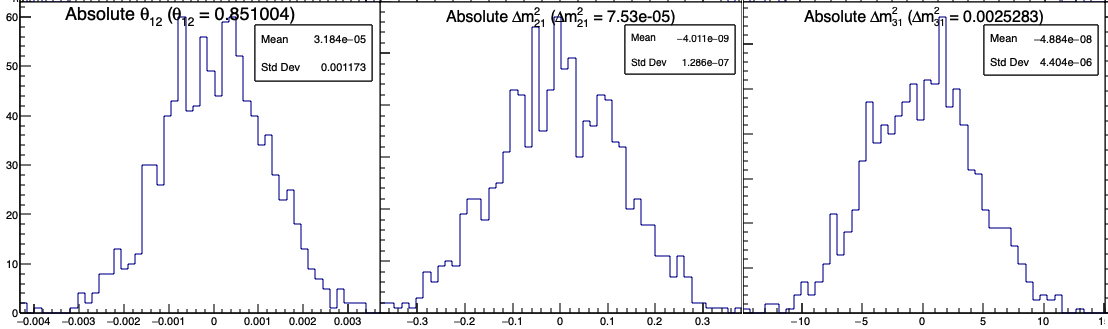
\includegraphics[width=\linewidth]{images/joint_fit/absolute_standard_joint_pearsonV.png}
  \caption{Distribution of BFP - nominal value for 1000 toy Standard joint fit. 6 years exposure, all background, \textbf{PearsonV} $\chi^2$, $\theta_{13}$ fixed. In those plots, $\theta_{12}$ stands for $\sin^2(2\theta_{12})$}
  \label{fig:joint_fit:abs_standard_pearsonV}
\end{figure}

\begin{figure}[ht]
  \centering
  \begin{subfigure}[t]{0.98\linewidth}
    \centering
    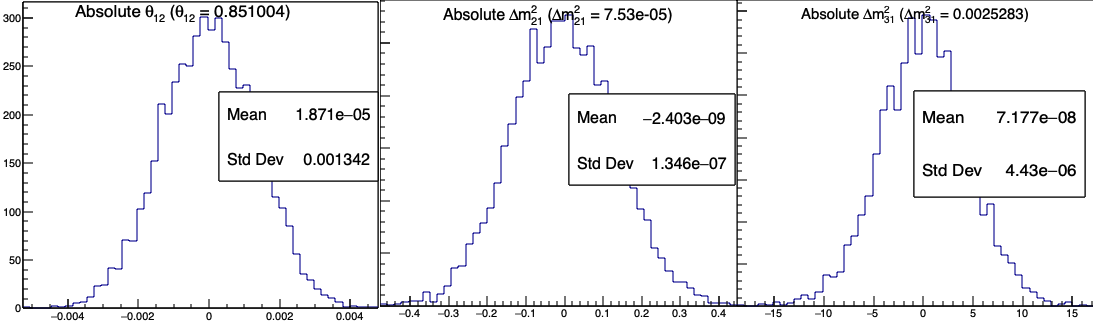
\includegraphics[width=\linewidth]{images/joint_fit/normal_delta_joint.png}
  \end{subfigure}

  \begin{subfigure}[t]{0.66\linewidth}
    \centering
    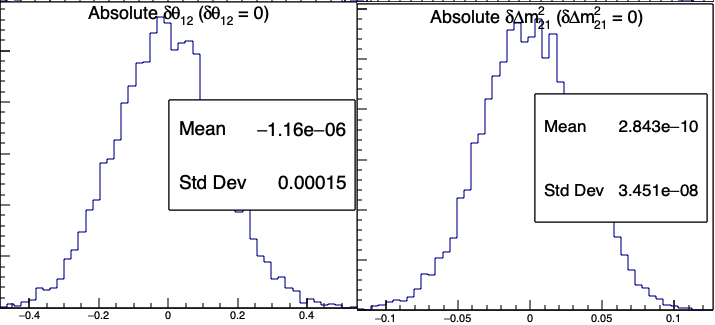
\includegraphics[width=\linewidth]{images/joint_fit/supp_delta_joint.png}
  \end{subfigure}

  \caption{Distribution of BFP - nominal value for 5000 toy Delta joint fit. 6 years exposure, all background, \textbf{PearsonV} $\chi^2$, $\theta_{13}$ fixed. In those plots, $\theta_{12}$ stands for $\sin^2(2\theta_{12})$ and $\delta \theta_{12}$ for $\delta \sin^2(\theta_{12})$}
  \label{fig:joint_fit:delta_fit}
\end{figure}

\subsubsection{Conclusion of the technical validation}

All the tests carried out in this section are consistent with our expectation. We therefore conclude that the technical implementation of the tools used in this chapter is correct.



%   (b) La matrice de covariance
%
%      i- méthode théorique
%         --- explications
%         --- résultats
%      ii- méthode toys
%             Idem
%      iii- la méthode basée sur les données sniper.
%            Idem
%      iv- comparaison
%         --- commentaires et conclusion.
%
%     Préciser ou rappeler ici que
%         --- pour nos tests, nous nous basons sur l'hypo H0 et donc nous générons la matrice sans QNL.
%         --- les corrélations dépendent peu de la forme du spectre ou se sa stat.
\section{Results}
\label{sec:joint_fit:results}

\subsection{Effect of supplementary QNL on the LPMT spectrum}

In this first part of this Section \ref{sec:joint_fit:results}, we will present the sensitivity of various test statistics to unexpected instrumental effects affecting the SPMT and LPMT differently. The latter effects will be illustrated by generated toy samples affected by the QNL effect.

Most of the tests involve either an individual fit to the LPMT spectrum or the SPMT spectrum, or a joint fit of these two spectra. To better understand why some test statistics turn out to be more powerful than others, we study briefly in the present subsection the results of these fits and interpret the differences.

We generate toy spectra, and fit them according to the default configuration described in Section \ref{sec:joint_fit:approach}.
During the generation of the LPMT spectrum, we distort it to simulated a QNL effect, with an intensity of $\alpha_{qnl}=1\%$. For reference, this is about three time the expected residual QNL after
the application of dual calorimetric calibration methods ($\alpha_{qnl} = 0.3\%$ \cite{juno_collaboration_calibration_2021}).

Backgrounds had to be ignored here: the JUNO inputs described in Section \ref{sec:joint_fit:framework} provide a reconstructed spectrum, but not the event per event information about the true $E_{vis}$, which we need to apply the QNL effect (See Equation \ref{eq:joint_fit:abc}).

The effect of this QNL on the spectrum is illustrated in Figure \ref{fig:joint_fit:anom_aqnl} In Table \ref{tab:joint_fit:qnl_results} we report the results of the different kinds of fits.

\begin{figure}[ht]
  \centering
  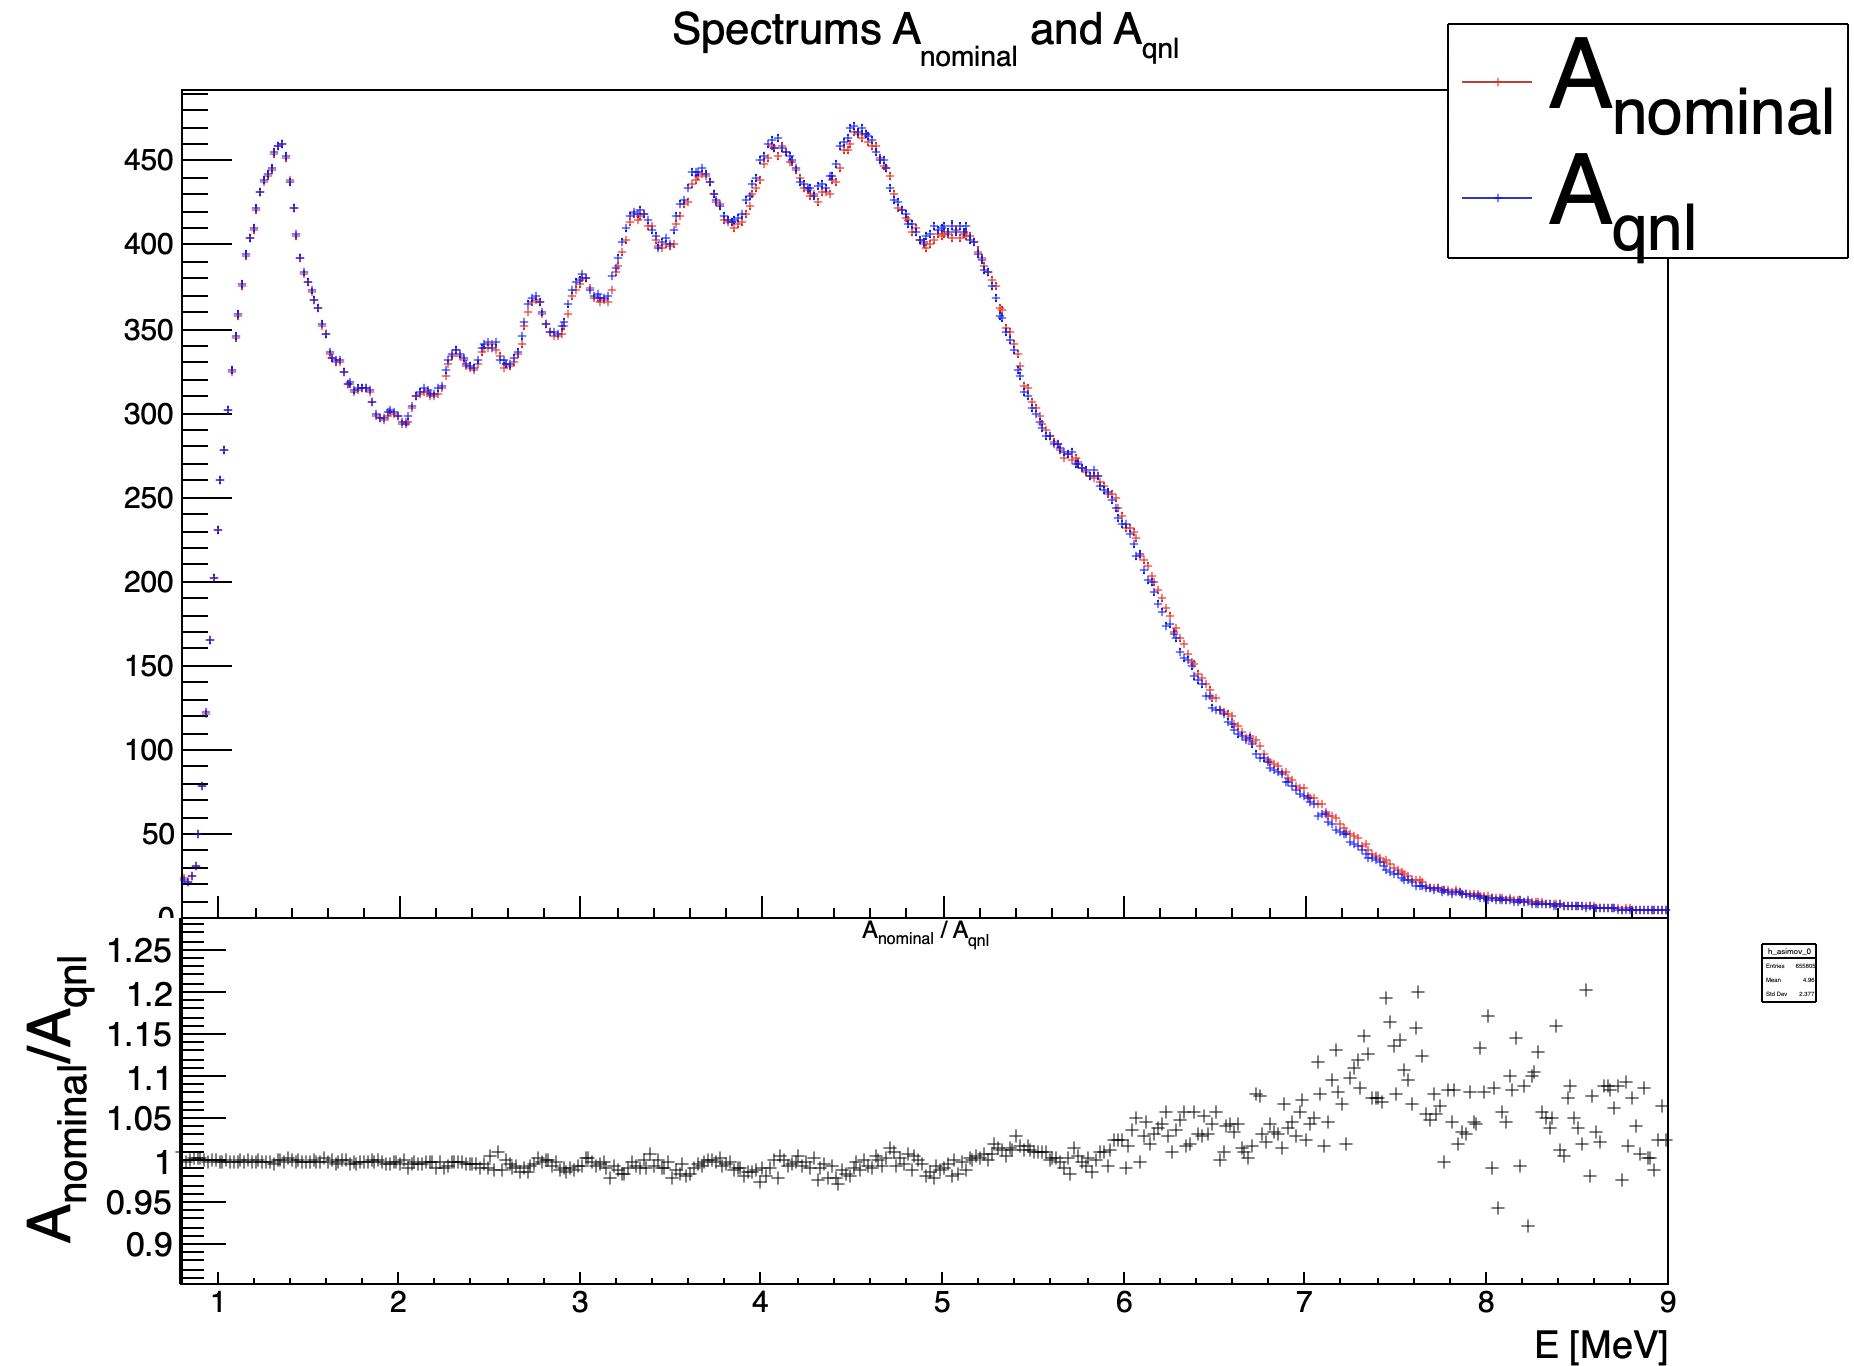
\includegraphics[height=6cm]{images/joint_fit/AnominalAQNL.png}
  \caption{\textbf{Top:} Theoretical spectrum without QNL (in red) and with $\alpha_{qnl} = 1\%$ (in blue). \textbf{Bottom:} Ratio between the theoretical spectrum with and without QNL.}
  \label{fig:joint_fit:anom_aqnl}
\end{figure}

We notice (1st line, first 3 columns) that the individual fit to the LPMT spectrum tends to find, as expected, biased value for $\Delta m^2_{21}$ and $\sin^2(2 \theta_{12})$ and $\Delta m^2_{31}$ (biased at about -1 sigma, -1.3 sigma and - 2.2 sigmas respectively). When a joint fit is performed, with the $\delta \Delta m^2_{21}$ and $\delta \sin^2(2 \theta_{12})$ fixed at 0, and ignoring in the computation of the $\chi^2$ the correlations between the LPMT and SPMT spectra, the biases on $\Delta m^2_{21}$ and $\sin^2(2 \theta_{12})$ (3rd line, first 3 columns) appear to be average of the biases seen by the individual fits to these spectra, a logical result since the individual sensitivities to these parameters are similar. The bias on $\Delta m^2_{31}$ (3rd column) remains the same as with the individual fit to the LPMT spectrum, however, which is expected since the SPMT spectrum carries no sensitivity to $\Delta m^2_{31}$.

When the joint fit is performed with the nominal covariance matrix (determined in Section \ref{sec:joint_fit:cov_mat} assuming no QNL), biases on
$\Delta m^2_{21}$ and $\sin^2(2 \theta_{12})$ explode: they are, respectively, about 6.5 and 2.5 times larger (4th line).

We explain it by the following mechanism : the fit tries to improve the agreement between the PDF and the data in the LPMT part of the spectrum by choosing biased values of the parameters. This in turn tends to deteriorate the agreement between the PDF and the SPMT spectrum (not distorted by QNL). In the end, a discrepancy remains between data and PDF in at least one sector (LPMT or SPMT) if not both. When the $\chi^2$ is built with a matrix which accounts for the correlations, this discrepancy can make the $\chi^2$ explode.

For instance, in some bins of the LPMT spectrum, we can imagine the PDF overestimates the QNL-distorted data, while the contrary happens in the corresponding bins of the SPMT spectrum. If the expected correlation is positive between these two bins, the $\chi^2$ will reach values accounting for a larger discrepancy than if no correlation existed and if only the raw agreement between the pdf and the spectra was important.

In reality, the consistency between the two can be judged only accounting for the correlations. This is the important role of the covariance matrix in this work. In other words, the spectra predictions are not only the $\bm{T}(\bm{\theta},\bm{\eta})$'s, but also the correlations.

\begin{table}[ht]
  \begin{footnotesize}
  \centering
  \begin{tabular}{l|lr|lr|lr|lr|lr|}
    Mean (std dev)  & \multicolumn{2}{c|}{$\theta_{12}$ [$10^{-3}$]} & \multicolumn{2}{c|}{$\Delta m^2_{21}$ [$10^{-7}\mathrm{eV}^{2}$]} & \multicolumn{2}{c|}{$\Delta m^2_{31}$ [$10^{-6}\mathrm{eV}^{2}$]} & \multicolumn{2}{c|}{$\delta \theta_{12}$ [$10^{-3}$]} & \multicolumn{2}{c|}{$\delta \Delta m^2_{21}$ [$10^{-7}\mathrm{eV}^{2}$]} \\
    \hline
    LPMT            & -1.569 & (1.171) & -0.957 & (0.989) & -8.235 & (3.898)       & \multicolumn{2}{c|}{Irrelevant} & \multicolumn{2}{c|}{Irrelevant}  \\
    SPMT            & -0.164 & (1.191) & -0.603 & (1.054) & \multicolumn{2}{c|}{Not sensitive} &\multicolumn{2}{c|}{Irrelevant} & \multicolumn{2}{c|}{Irrelevant}  \\
    Indep Standard  & -0.880 & (1.174) & -0.786 & (1.004) & -8.195 & (3.900)       & \multicolumn{2}{c|}{Irrelevant} & \multicolumn{2}{c|}{Irrelevant}  \\
    Standard        & -8.106 & (1.423) & -2.483 & (1.018) & -6.649 & (4.008)       & \multicolumn{2}{c|}{Irrelevant} & \multicolumn{2}{c|}{Irrelevant}  \\
    Indep Delta     & -0.169 & (1.190) & -0.598 & (1.054) & -8.234 & (3.899)       & -1.397 & (0.259)     & -0.361 & (0.366) \\
    Delta           & -0.163 & (1.183) & -1.532 & (1.036) & -8.193 & (3.934)       & -1.441 & (0.193)     & 0.654  & (0.303) \\
  \end{tabular}
  \end{footnotesize}
  \caption{In each column, the mean of the distribution of the 1000 best fit values found by fitting the 1000 toy samples with $\alpha_{qnl} = 1\%$ is shown, from which we subtracted the value assumed when generating the toys. A value different from 0 indicates a bias. Between bracket, the average uncertainty of the fitted value is also shown. It allows to judge of the severity of the bias. For instance, the measurement of $\sin^2(2 \theta_{12})$ by fitting only the LPMT spectrum tends to be biased at the -1.569/1.171 = - 1.34 sigma. }
  \label{tab:joint_fit:qnl_results}
\end{table}


Another point must be noted : the correlation matrix $V$ is evaluated assuming no QNL. With the QNL effect added, the actual correlations between the LPMT and SPMT generated toy spectra is a bit different, adding another source of discrepancy between the data and the predictions, and further increasing the $\chi^2$.

All in all, the minimisation of the $\chi^2$ requires a larger scan of the oscillation parameters values than when correlations are ignored. Values can be chosen which are farther from the nominal ones, meaning larger biases.

This is actually an advantage. Indeed, we can see in table \ref{tab:joint_fit:qnl_results} that when $\delta \Delta m^2_{21}$ and $\delta \sin^2(2 \theta_{12})$ are allowed to float in the fit, they "absorb" a large part of the bias. Notice in particular that adding the value of $\delta \Delta m^2_{21}$ to the remaining bias on $\Delta m^2_{21}$ (last line, columns 1 and 4) one retrieves the bias of the individual fit to the LPMT spectrum. The same applies to $\sin^2(2\theta_{12})$. Consequently, large values of $\delta \Delta m^2_{21}$ and  $\delta \sin^2(2 \theta_{12})$ are expected, hence high significances to help us to detect the distortion. In this case (last line, column 4 and 5), we see the most probable values of the fitted $\delta \Delta m^2_{21}$ and $\delta \sin^2(2 \theta_{12})$ parameters differ from zero at about 7.46 sigma and 2.2 sigma.

Based on the above observations, we expect the "$\chi^2_{H_0}-\chi^2_{H_1}$" and "Distributions of $\delta \Delta m^2_{21}$
and  $\delta \sin^2(2 \theta_{12})$" test statistics described in sections \ref{sec:joint_fit:hypothesis} and \ref{sec:joint_fit:delta_distrib} to have the highest power.
The "Direct comparison between the SPMT and LPMT spectra" should perform in the same ballpark. Finally, the "Comparison of individual fits" is expected to be have less power.

\subsection{Comparison and statistical tests results}

I present in this following Subsection the results from the tests and comparison detailed in section \ref{sec:joint_fit:approach}. For each distribution we compute the median p-value with respect to the distribution ${\cal D}(\alpha_{qnl} = 0\%)$. For this, we compute the median value of the distribution of interest ${\cal D}(\alpha_{qnl})$, then compute the p value
\begin{equation}
  p = \frac{N({\cal D}(0) > \text{Median}[{\cal D}(\alpha_{qnl})])}{N_{tot}}
\end{equation}
where $N({\cal D}(0) > \text{Median}[{\cal D}(\alpha_{qnl})])$ is the number of toy in the distribution ${\cal D}(\alpha_{qnl} = 0\%)$ that have a greater value than the median of the ${\cal D}(\alpha_{qnl})$. The p-value represent the probability for a non perturbed event to do worse that the median perturbed event.

The uncertainty on the p-value is computed using
\begin{equation}
  \sigma p = \sqrt{\frac{p(1-p)}{N}}
\end{equation}
which do not account for all uncertainties but serves as indicator.

\subsubsection{Comparison of solar parameters from individual analysis: $\chi^2_{ind}$}

The results are presented in Figure \ref{fig:joint_fit:chi2_ind}. We see that the p-value are much less significant than the other tests, this is because this test possess much less information about the relation between the LPMT and SPMT systems.

\begin{figure}[th]
  \centering
  \begin{subfigure}[t]{0.48\linewidth}
    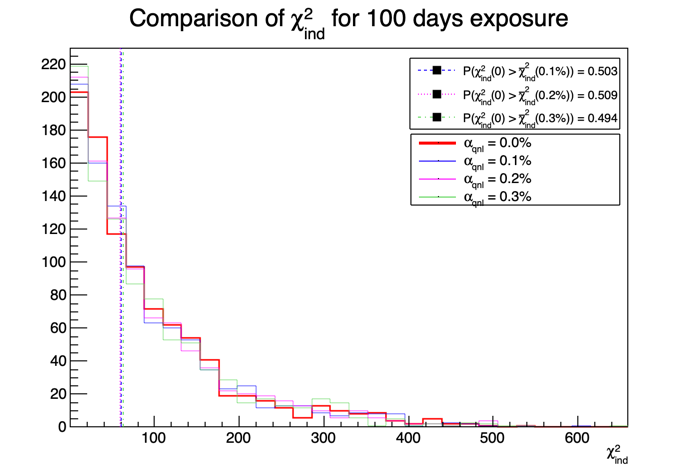
\includegraphics[width=\linewidth]{images/joint_fit/stat_tests/chi2_ind_100d.png}
  \end{subfigure}
  \begin{subfigure}[t]{0.48\linewidth}
    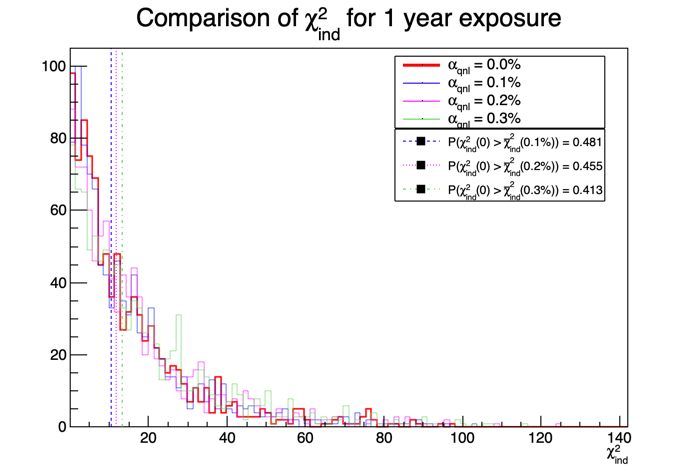
\includegraphics[width=\linewidth]{images/joint_fit/stat_tests/chi2_ind_1y.png}
  \end{subfigure}


  \begin{subfigure}[t]{0.48\linewidth}
    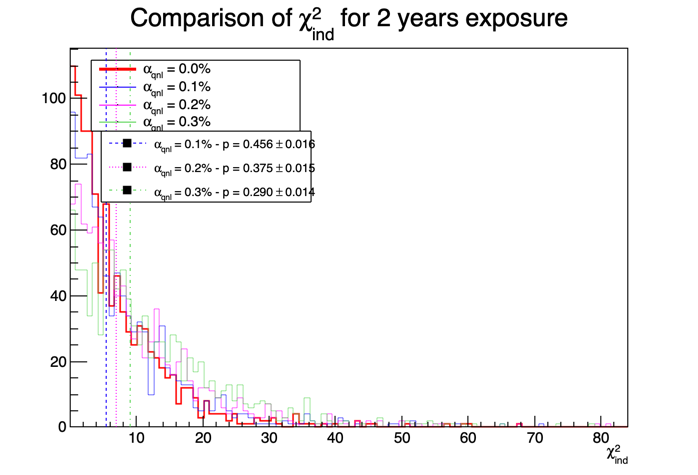
\includegraphics[width=\linewidth]{images/joint_fit/stat_tests/chi2_ind_2y.png}
  \end{subfigure}
  \begin{subfigure}[t]{0.48\linewidth}
    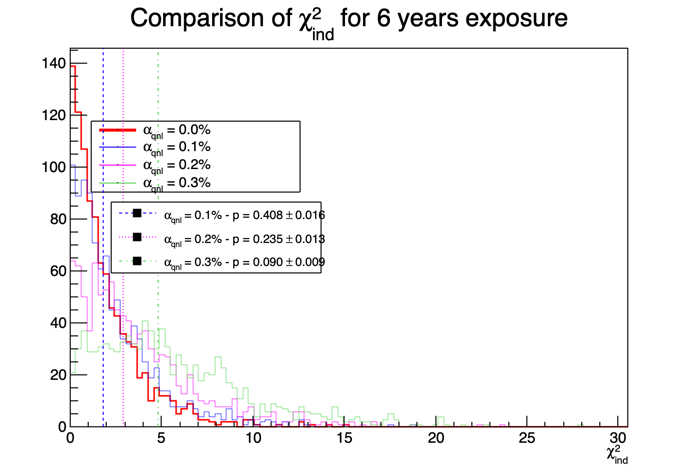
\includegraphics[width=\linewidth]{images/joint_fit/stat_tests/chi2_ind_6y.png}
  \end{subfigure}
  \caption{Distribution of the $\chi^2_{ind}$ for 1000 toys for different exposures. The dashed lines represent the median of the distributions and the p-value are the percentage of the $\alpha_{qnl} = 0$ distribution that are greater than those medians.}
  \label{fig:joint_fit:chi2_ind}
\end{figure}

This test is the most straightforward as it require only the fit of the two spectra and the estimation of the parameters covariances, but is also the less powerful with a p value for $\alpha_{qnl} = 0.3\%$ of $0.09 \pm 0.009$ at 6 years.


\subsubsection{Direct comparison between the LPMT and SPMT spectra: $\chi^2_{spe}$}

The results for different exposures can be found in Figure \ref{fig:joint_fit:chi2_spec}. To give an idea of the significance of this test, we provide the median p-value for each test $\alpha_{qnl} \neq 0$. As expected, the power of this test rises as the exposure does. We see significant discrimination at 6 years for $\alpha_{qnl} \geq 0.3 \%$ where the p-value for $\alpha_{qnl} = 0.3\%$ is $0.005 \pm 0.0022$.


\begin{figure}[th]
  \centering
  \begin{subfigure}[t]{0.48\linewidth}
    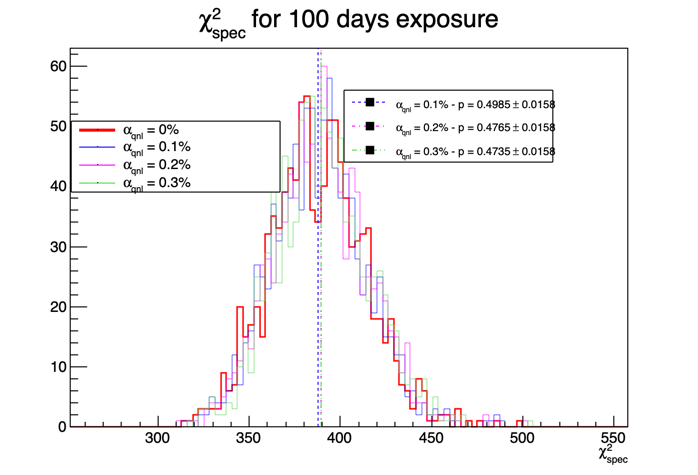
\includegraphics[width=\linewidth]{images/joint_fit/stat_tests/chi2_spec_100d.png}
  \end{subfigure}
  \begin{subfigure}[t]{0.48\linewidth}
    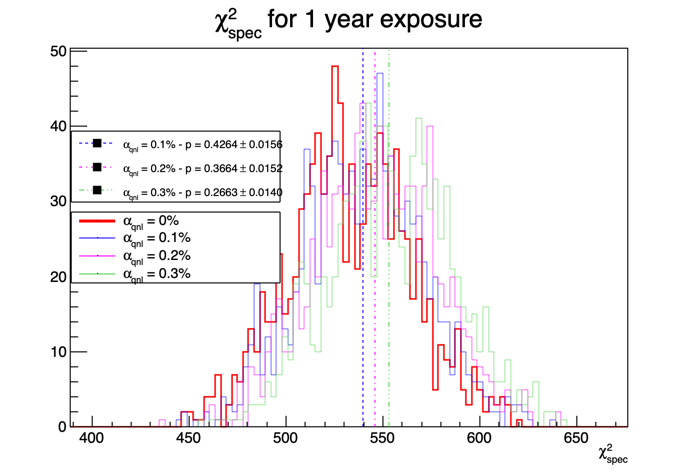
\includegraphics[width=\linewidth]{images/joint_fit/stat_tests/chi2_spec_1y.png}
  \end{subfigure}


  \begin{subfigure}[t]{0.48\linewidth}
    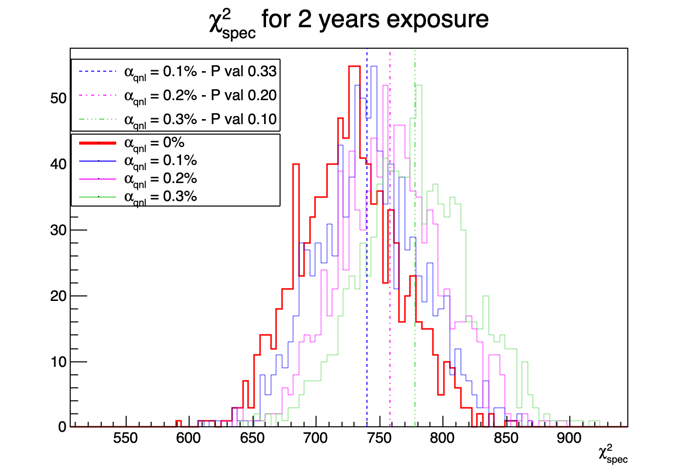
\includegraphics[width=\linewidth]{images/joint_fit/stat_tests/chi2_spec_2y.png}
  \end{subfigure}
  \begin{subfigure}[t]{0.48\linewidth}
    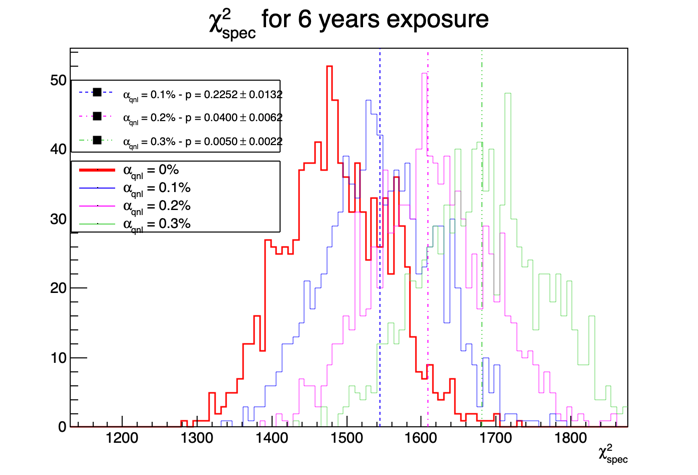
\includegraphics[width=\linewidth]{images/joint_fit/stat_tests/chi2_spec_6y.png}
  \end{subfigure}
  \caption{Distribution of the $\chi^2_{spe}$ for 1000 toys for different exposure. The dashed line represent the median of the distribution and the p-value are the percentage of the $\alpha_{qnl} = 0$ distribution that are greater than those medians.}
  \label{fig:joint_fit:chi2_spec}
\end{figure}

This test relies solely on the estimated covariance matrix between the two spectra, requiring no fitting. As a result, it is a very lightweight test that can still provide valuable indications of potential unknown distortions between the two spectra.

\subsubsection{Joint fit: $\chi^2_{H_0} - \chi^2_{H_1}$}
This test is the most complex, requiring two fit and the covariance matrix between the LPMT and SPMT spectra. The results are presented in Figure \ref{fig:joint_fit:chi2_H}.

\begin{figure}[th]
  \centering
  \begin{subfigure}[t]{0.48\linewidth}
    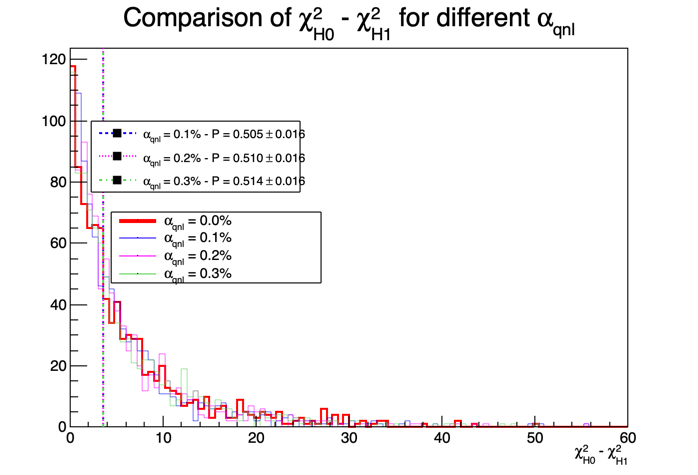
\includegraphics[width=\linewidth]{images/joint_fit/stat_tests/chi2_H_100d.png}
    \caption{100 days exposure}
  \end{subfigure}
  \begin{subfigure}[t]{0.48\linewidth}
    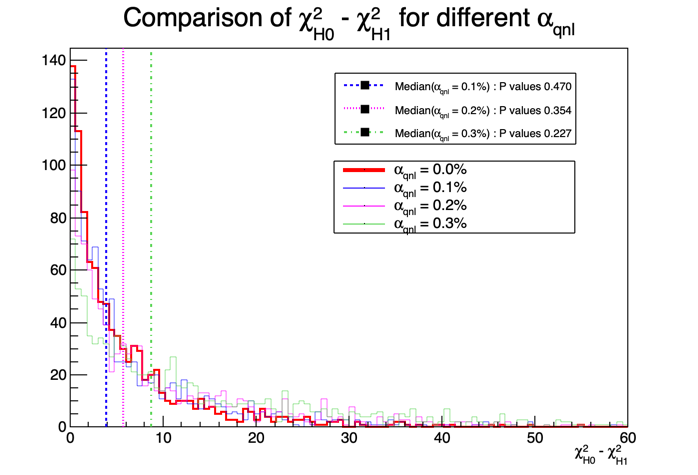
\includegraphics[width=\linewidth]{images/joint_fit/stat_tests/chi2_H_1y.png}
    \caption{1 year exposure}
  \end{subfigure}


  \begin{subfigure}[t]{0.48\linewidth}
    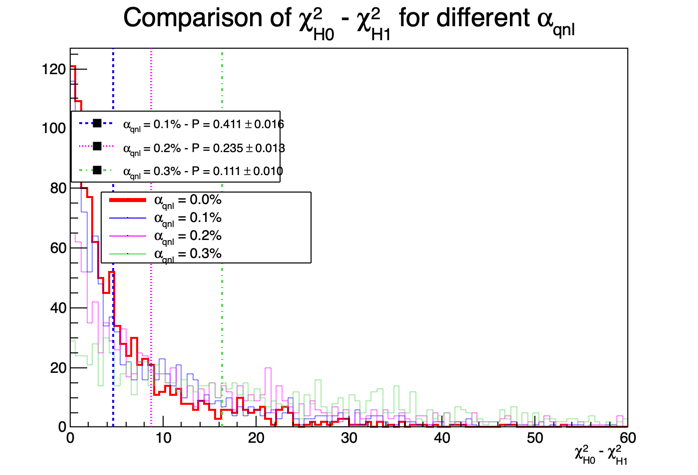
\includegraphics[width=\linewidth]{images/joint_fit/stat_tests/chi2_H_2y.png}
    \caption{2 years exposure}
  \end{subfigure}
  \begin{subfigure}[t]{0.48\linewidth}
    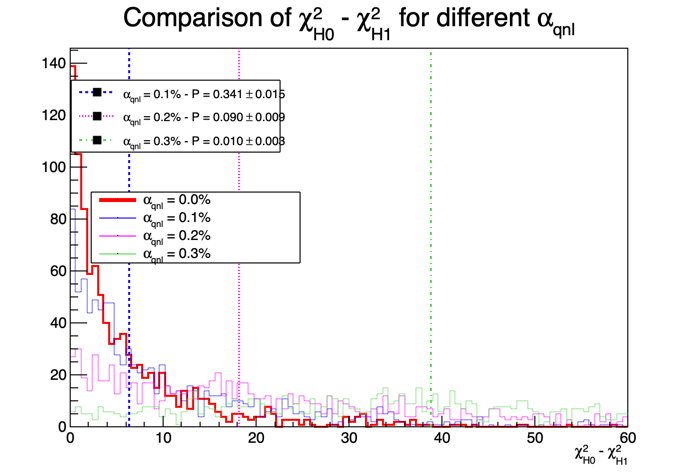
\includegraphics[width=\linewidth]{images/joint_fit/stat_tests/chi2_H_6y.png}
    \caption{6 years exposure}
  \end{subfigure}
  \caption{Distribution of $\chi^2_{H_0} - \chi^2_{H_1}$ for 1000 toys for different exposure. The dashed line represent the median of the distribution and the p-value are the percentage of the $\alpha_{qnl} = 0$ distribution that are greater than those medians.}
  \label{fig:joint_fit:chi2_H}
\end{figure}

The results are good, close to the $\chi^2_{spe}$, one with a p-value at 6 years for $\alpha_{qnl} = 0.3\%$ of $0.01 \pm 0.003$. This sensitivity is consistent with that of $\chi^2_{spe}$.

\subsubsection{Comparison of the parameters $\delta \sin^2(2\theta_{12})$ and $\delta \Delta m^2_{21}$}

We can see that the $\delta \Delta m^2_{21}$ has a very small discriminative power (Figure \ref{fig:joint_fit:chi2_delta_m}) even at 6 years exposure with a p-value of $0.34 \pm 0.01$ for $\alpha_{qnl} = 0.3\%$. On the other hand $\delta \theta_{12}$ (Figure \ref{fig:joint_fit:chi2_delta}) has much more discriminative power with a p-value for $\alpha_{qnl} = 0.3\%$ of $0.025 \pm 0.005$. This test with a single joint fit seems to be still less powerful than the $\chi^2_{spe}$. This can be explained as this method only get information through the oscillation parameters $\theta_{12}$ and $\Delta m^2_{21}$ missing potential informations contained in $\Delta m^2_{31}$.


\begin{figure}[th]
  \centering
  \begin{subfigure}[t]{0.48\linewidth}
    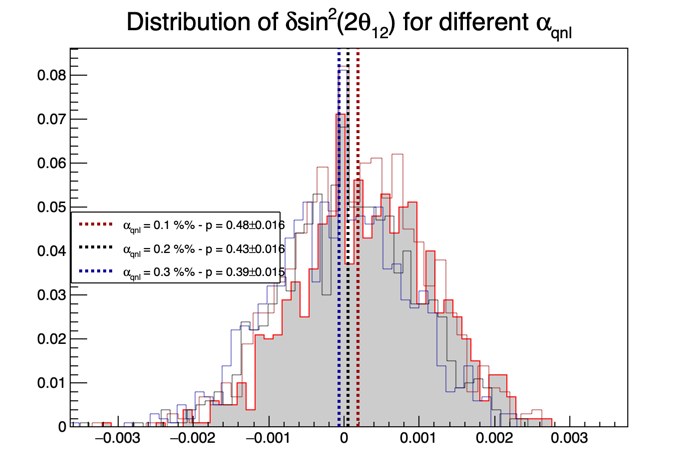
\includegraphics[width=\linewidth]{images/joint_fit/stat_tests/chi2_delta_100d.png}
    \caption{100 days exposure}
  \end{subfigure}
  \begin{subfigure}[t]{0.48\linewidth}
    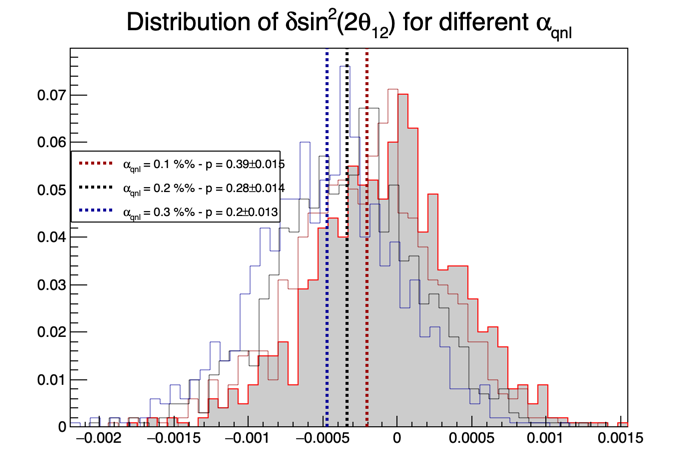
\includegraphics[width=\linewidth]{images/joint_fit/stat_tests/chi2_delta_1y.png}
    \caption{1 year exposure}
  \end{subfigure}


  \begin{subfigure}[t]{0.48\linewidth}
    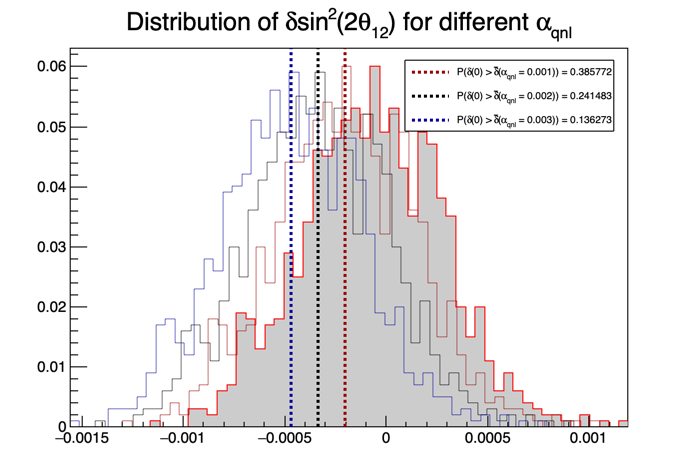
\includegraphics[width=\linewidth]{images/joint_fit/stat_tests/chi2_delta_2y.png}
    \caption{2 years exposure}
  \end{subfigure}
  \begin{subfigure}[t]{0.48\linewidth}
    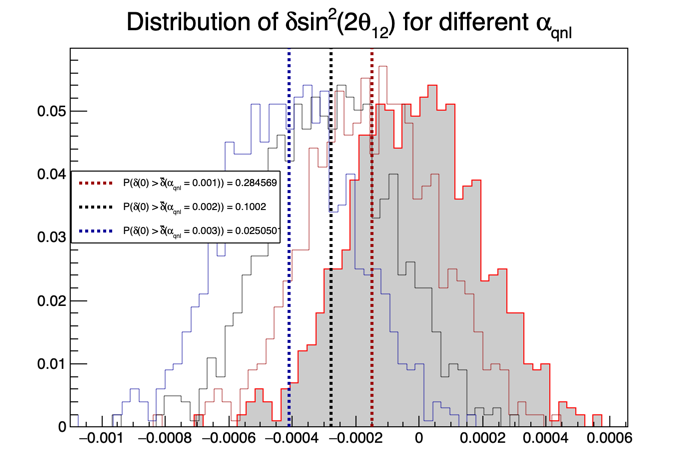
\includegraphics[width=\linewidth]{images/joint_fit/stat_tests/chi2_delta_6y.png}
    \caption{6 years exposure}
  \end{subfigure}
  \caption{Distribution of the $\delta \sin^2(2\theta_{12})$ for 1000 toys for different exposure. The dashed line represent the median of the distribution and the p-value are the percentage of the $\alpha_{qnl} = 0$ distribution that are greater than those medians.}
  \label{fig:joint_fit:chi2_delta}
\end{figure}


\begin{figure}[th]
  \centering
  \begin{subfigure}[t]{0.48\linewidth}
    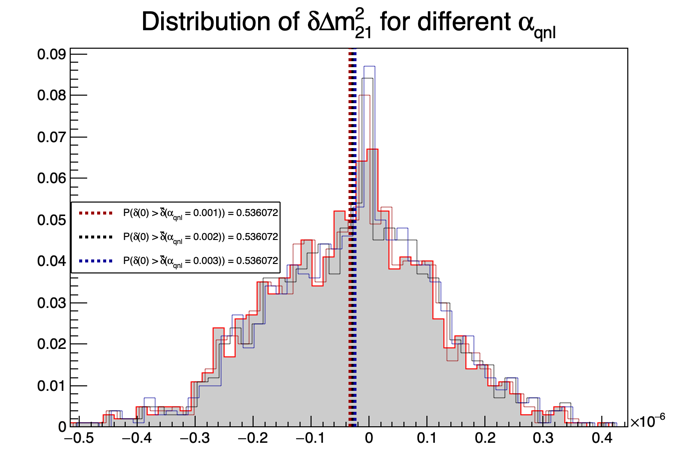
\includegraphics[width=\linewidth]{images/joint_fit/stat_tests/chi2_delta_m_100d.png}
    \caption{100 days exposure}
  \end{subfigure}
  \begin{subfigure}[t]{0.48\linewidth}
    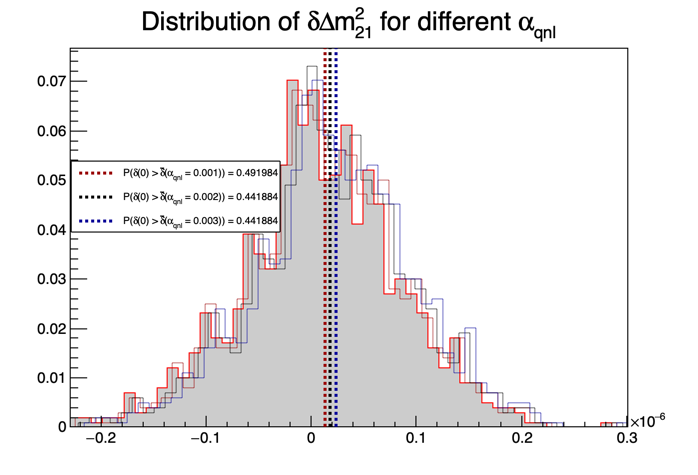
\includegraphics[width=\linewidth]{images/joint_fit/stat_tests/chi2_delta_m_1y.png}
    \caption{1 year exposure}
  \end{subfigure}


  \begin{subfigure}[t]{0.48\linewidth}
    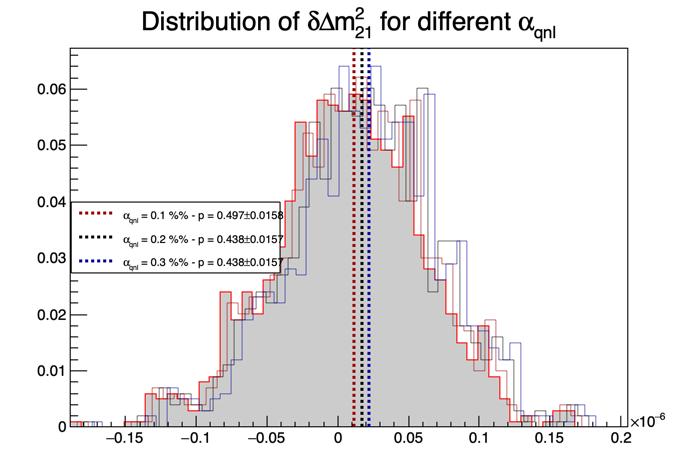
\includegraphics[width=\linewidth]{images/joint_fit/stat_tests/chi2_delta_m_2y.png}
    \caption{2 years exposure}
  \end{subfigure}
  \begin{subfigure}[t]{0.48\linewidth}
    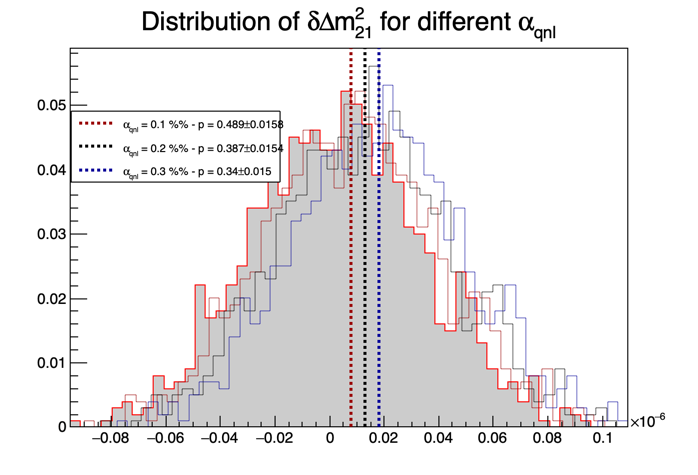
\includegraphics[width=\linewidth]{images/joint_fit/stat_tests/chi2_delta_m_6y.png}
    \caption{6 years exposure}
  \end{subfigure}
  \caption{Distribution of the $\delta \Delta m^2_{21}$ for 1000 toys for different exposure. The dashed line represent the median of the distribution and the p-value are the percentage of the $\alpha_{qnl} = 0$ distribution that are greater than those medians.}
  \label{fig:joint_fit:chi2_delta_m}
\end{figure}

\subsubsection{Summary}

The p-values from the different test and comparison for $\alpha_{qnl} = 0.3\%$ are reported in Table \ref{tab:joint_fit:results:p_value}.
\begin{table}[ht]
  \centering
  \begin{tabular}{l | c | c | c | c}
                                   & 100 days          & 1 year           & 2 years          & 6 years \\
                                   \hline
    $\chi^2_{ind}$                               & $0.49$  & $0.41 $ & $0.29$ & $0.090$ \\
    $\chi^2_{spec}$                              & $0.47$  & $0.27 $ & $\bm{0.10}$ & $\bm{0.005}$ \\
    $\chi^2_{H_0} - \chi^2_{H_1}$                & $0.51$  & $0.23 $ & $\bm{0.11}$ & $\bm{0.010}$ \\
    Comparison of $\delta \sin^2(2 \theta_{12})$ & $0.39$  & $0.2  $ & $0.14$ & $0.025$ \\
  \end{tabular}
  \caption{Report of the p-value of the different tests and comparisons for $\alpha_{qnl} = 0.3\%$ for the different exposures.}
  \label{tab:joint_fit:results:p_value}
\end{table}

% Montre chi^2_{spe} 335 ?

%
%   (c) Résultats fit séparés
%
%
%   (d) Résultats fits joints
%
%   (e) Résultats avec corrélations reco_spmt vs. reco_lmpt mieux prises en compte
%

\section{Conclusion and perspectives}
\label{sec:joint_fit:conclusion}
% Vll) Discussions, perspectives

In this chapter, we present the development of a fit framework that allows us to fit multiple spectra simultaneously. We also introduce a set of tools that enable us to detect potential distortions in one of the two spectra. As an illustration of the capability of these tools, we use supplementary event-wise non-linearity and compare it to the potential residual event-wise non-linearity after calibration.

Table \ref{tab:joint_fit:results:p_value} gives a synthetic view of the strength of our methods. As expected, two methods that exploit the knowledge of the correlations between the SPMT and LPMT spectra obtain the best results. At high exposures, if the QNL effects are not calibrated out as well as expected ($>0.3\%$), our best test statistics will be likely to detect them (median p-values below 10\% after 2 years of data taking,  about 1\% after 6 years).
In case of major effect (QNL or another unexpected instrumental effect) is worse , the detection will be even more likely.  Below two years of data taking, only large unexpected instrumental effects can be detected.

One of JUNO most important goals is to determine the NMO independently of other experiments. This should not happen before 6 years of data taking. Our results demonstrate that dual calorimetry with neutrino oscillation can be a useful approach to help ensure the robustness of this result.

\subsection{Empirical correlation matrix from fully simulated event}

As already explained several times, one of the limitation of this work is that we assume the SPMT and LPMT energy reconstructions to be totally uncorrelated. In reality, this is not true. The $V$ covariance matrix used in the test statistics should therefore be evaluated accounting for this. This involves complications that make the subject out of the scope of this thesis. We present here a brief study which goal is to get a rough idea of the impact of these reconstruction correlations.

The core of the idea is that the LPMT and SPMT reconstruction errors is bound to be correlated due to systematic effects. The first and most obvious one, for example, is energy escaping from the central detector. If the positron, or one of the two annihilation gamma, escape from the detector, less energy is deposited thus both of the systems will reconstruct a lower energy that was actually deposited. On a more subtle scale, the randomness in the production of scintillation photons is common for the two systems, if the liquid scintillator produces fewer scintillation photons for an event, both systems are likely to underestimate the energy.

We study those effects by computing from a dataset of IBD events, uniformly distributed in the CD, the correlation between the reconstruction errors on the energy
\begin{equation}
  Corr(E^{lpmt}_{rec} - E_{vis}, E^{spmt}_{rec} - E_{vis})
\end{equation}
where $E^{lpmt}_{rec}$ and $E^{spmt}_{rec}$ are the reconstructed energies from both systems and $E_{vis}$ the true visible energy. The OMILREC algorithm, presented in section \ref{sec:juno:reco}, is used for the LPMT reconstruction $E^{lpmt}_{rec}$, and the CNN presented in Chapter \ref{sec:jcnn} for the SPMT reconstruction $E^{spmt}_{rec}$.

%With this observable, the bias difference between the two reconstructions at fixed $R$ and $E$ is irrelevant. However, since we compute the correlation in $E$ and $R^3$ bins, we need to account for the potential spurious relationship between the errors and their respective biases. If the bias is small relative to the resolution, it can be ignored; but if the bias variation is on the same order of magnitude as the error, it may introduce false correlations. For this reason, based on the CNN results shown in Figure \ref{fig:jcnn:vic_cnn}, we restrict our analysis to the $1 < E_{dep} < 9$ MeV range.

The results of those correlations are presented in Figure \ref{fig:joint_fit:empirical_corr:E_a_R} for the single energy and the interaction radius dependency, and Figure \ref{fig:joint_fit:empirical_corr:E_R} for the dual energy and interaction radius dependencies.

\begin{figure}[ht]
  \centering
  \begin{subfigure}[t]{0.48\linewidth}
    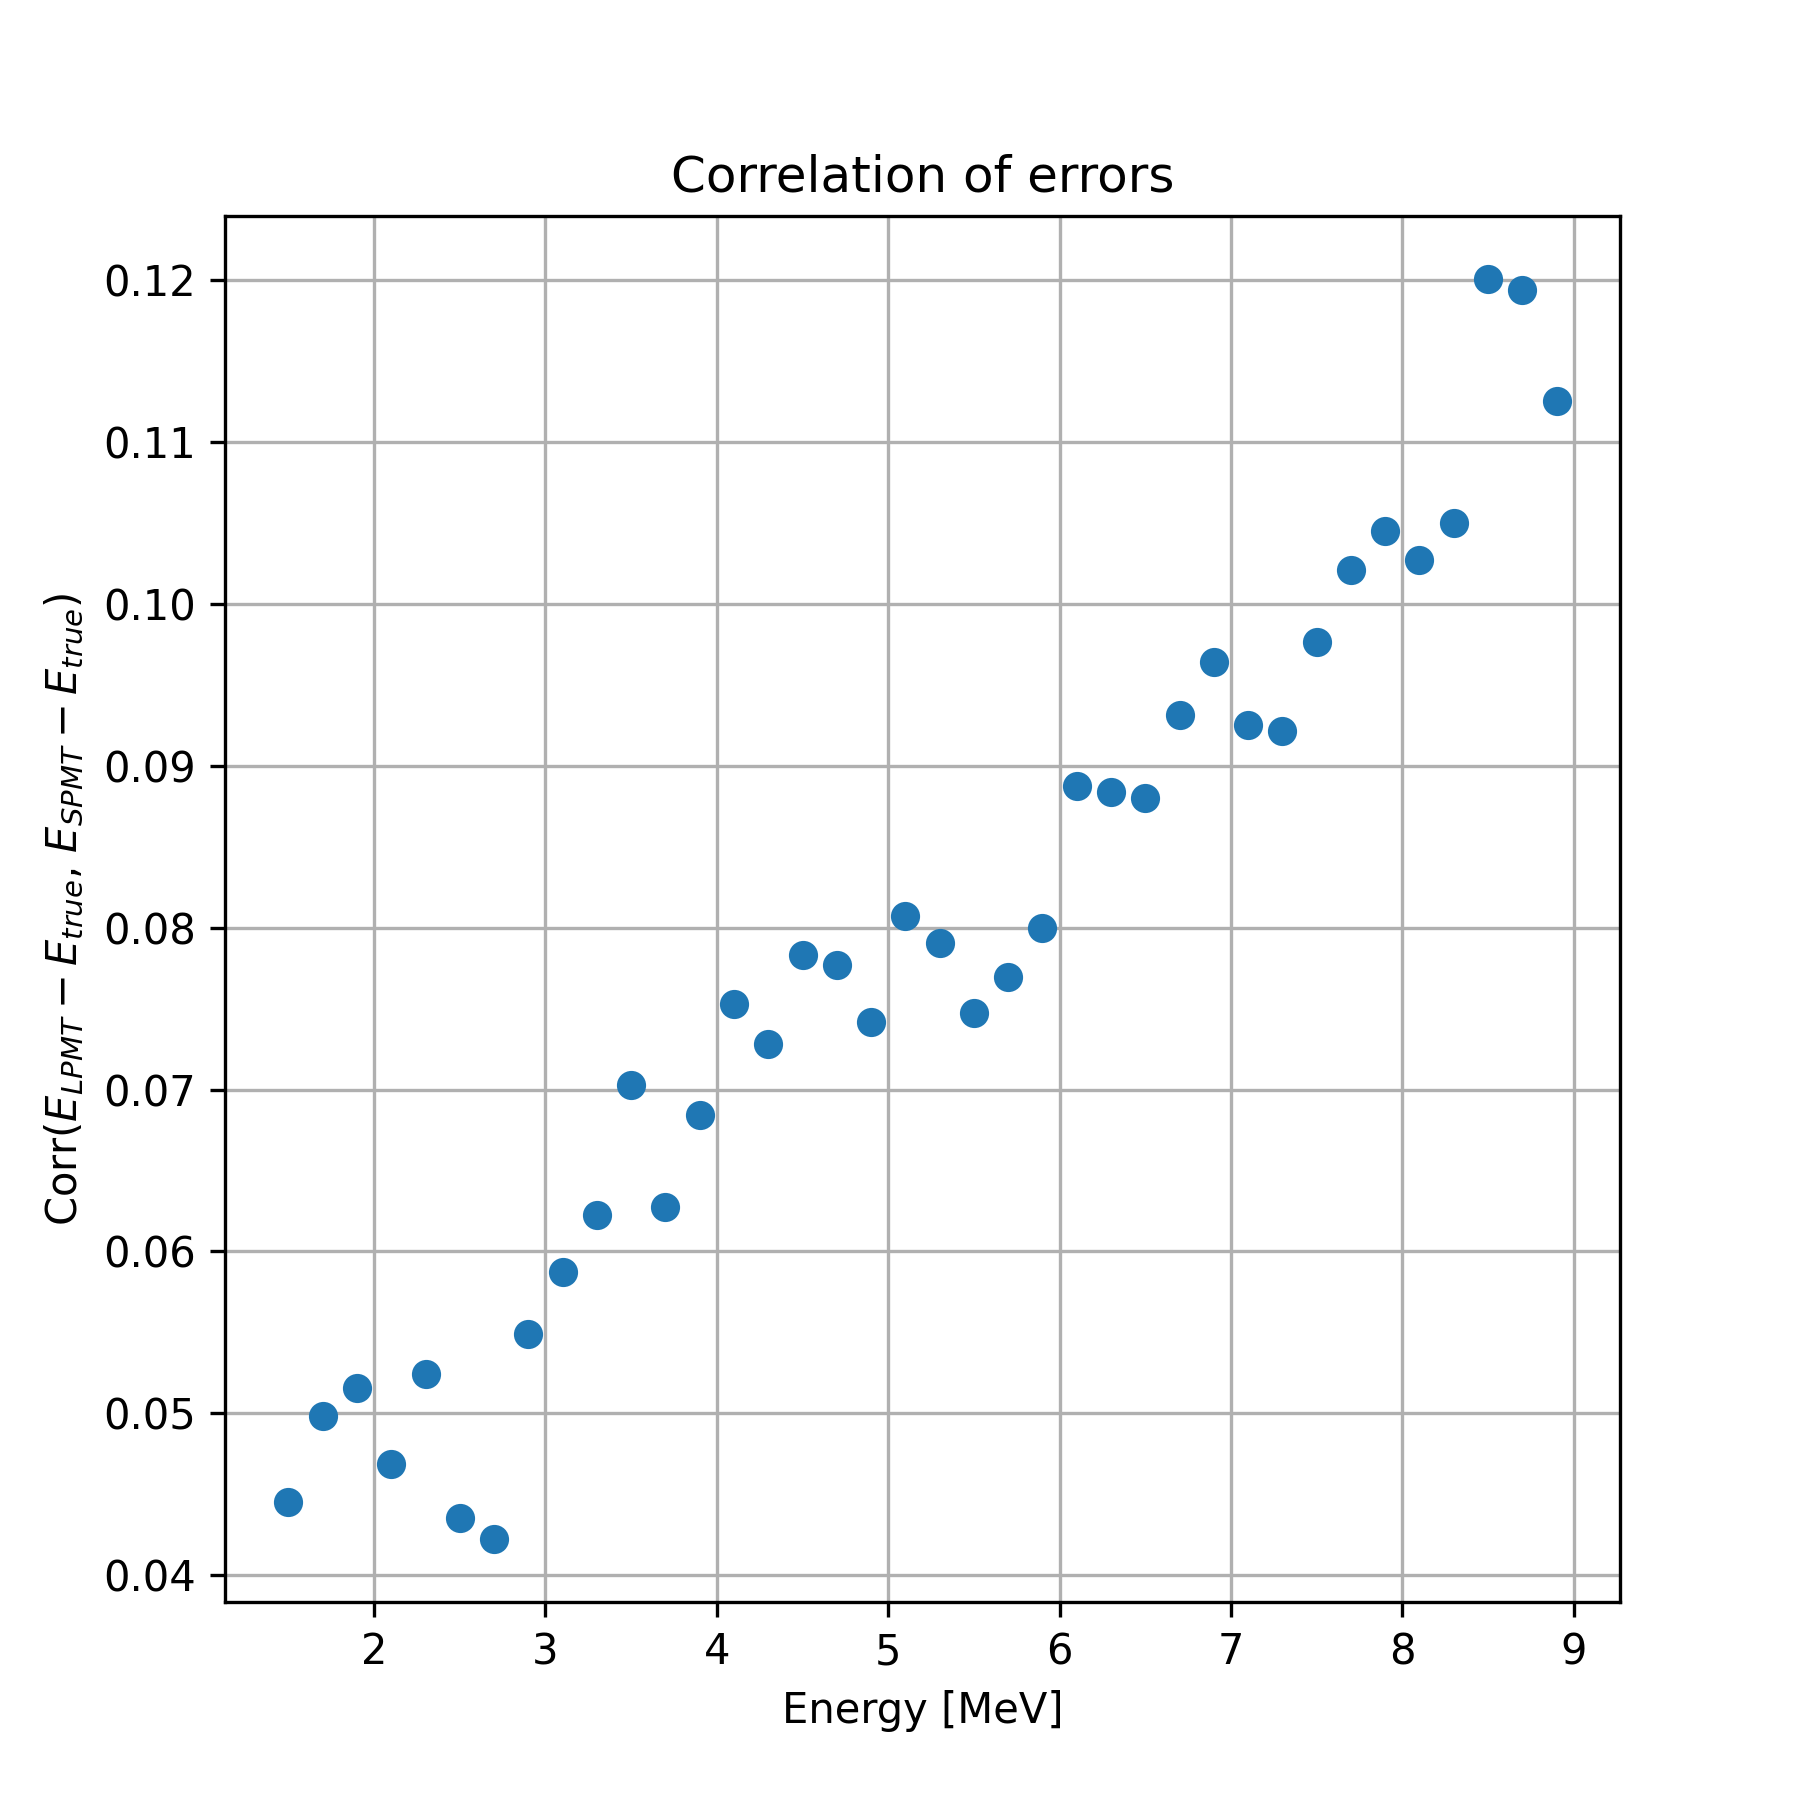
\includegraphics[width=\linewidth]{images/joint_fit/E_corr.png}
  \end{subfigure}
  \hfill
  \begin{subfigure}[t]{0.48\linewidth}
    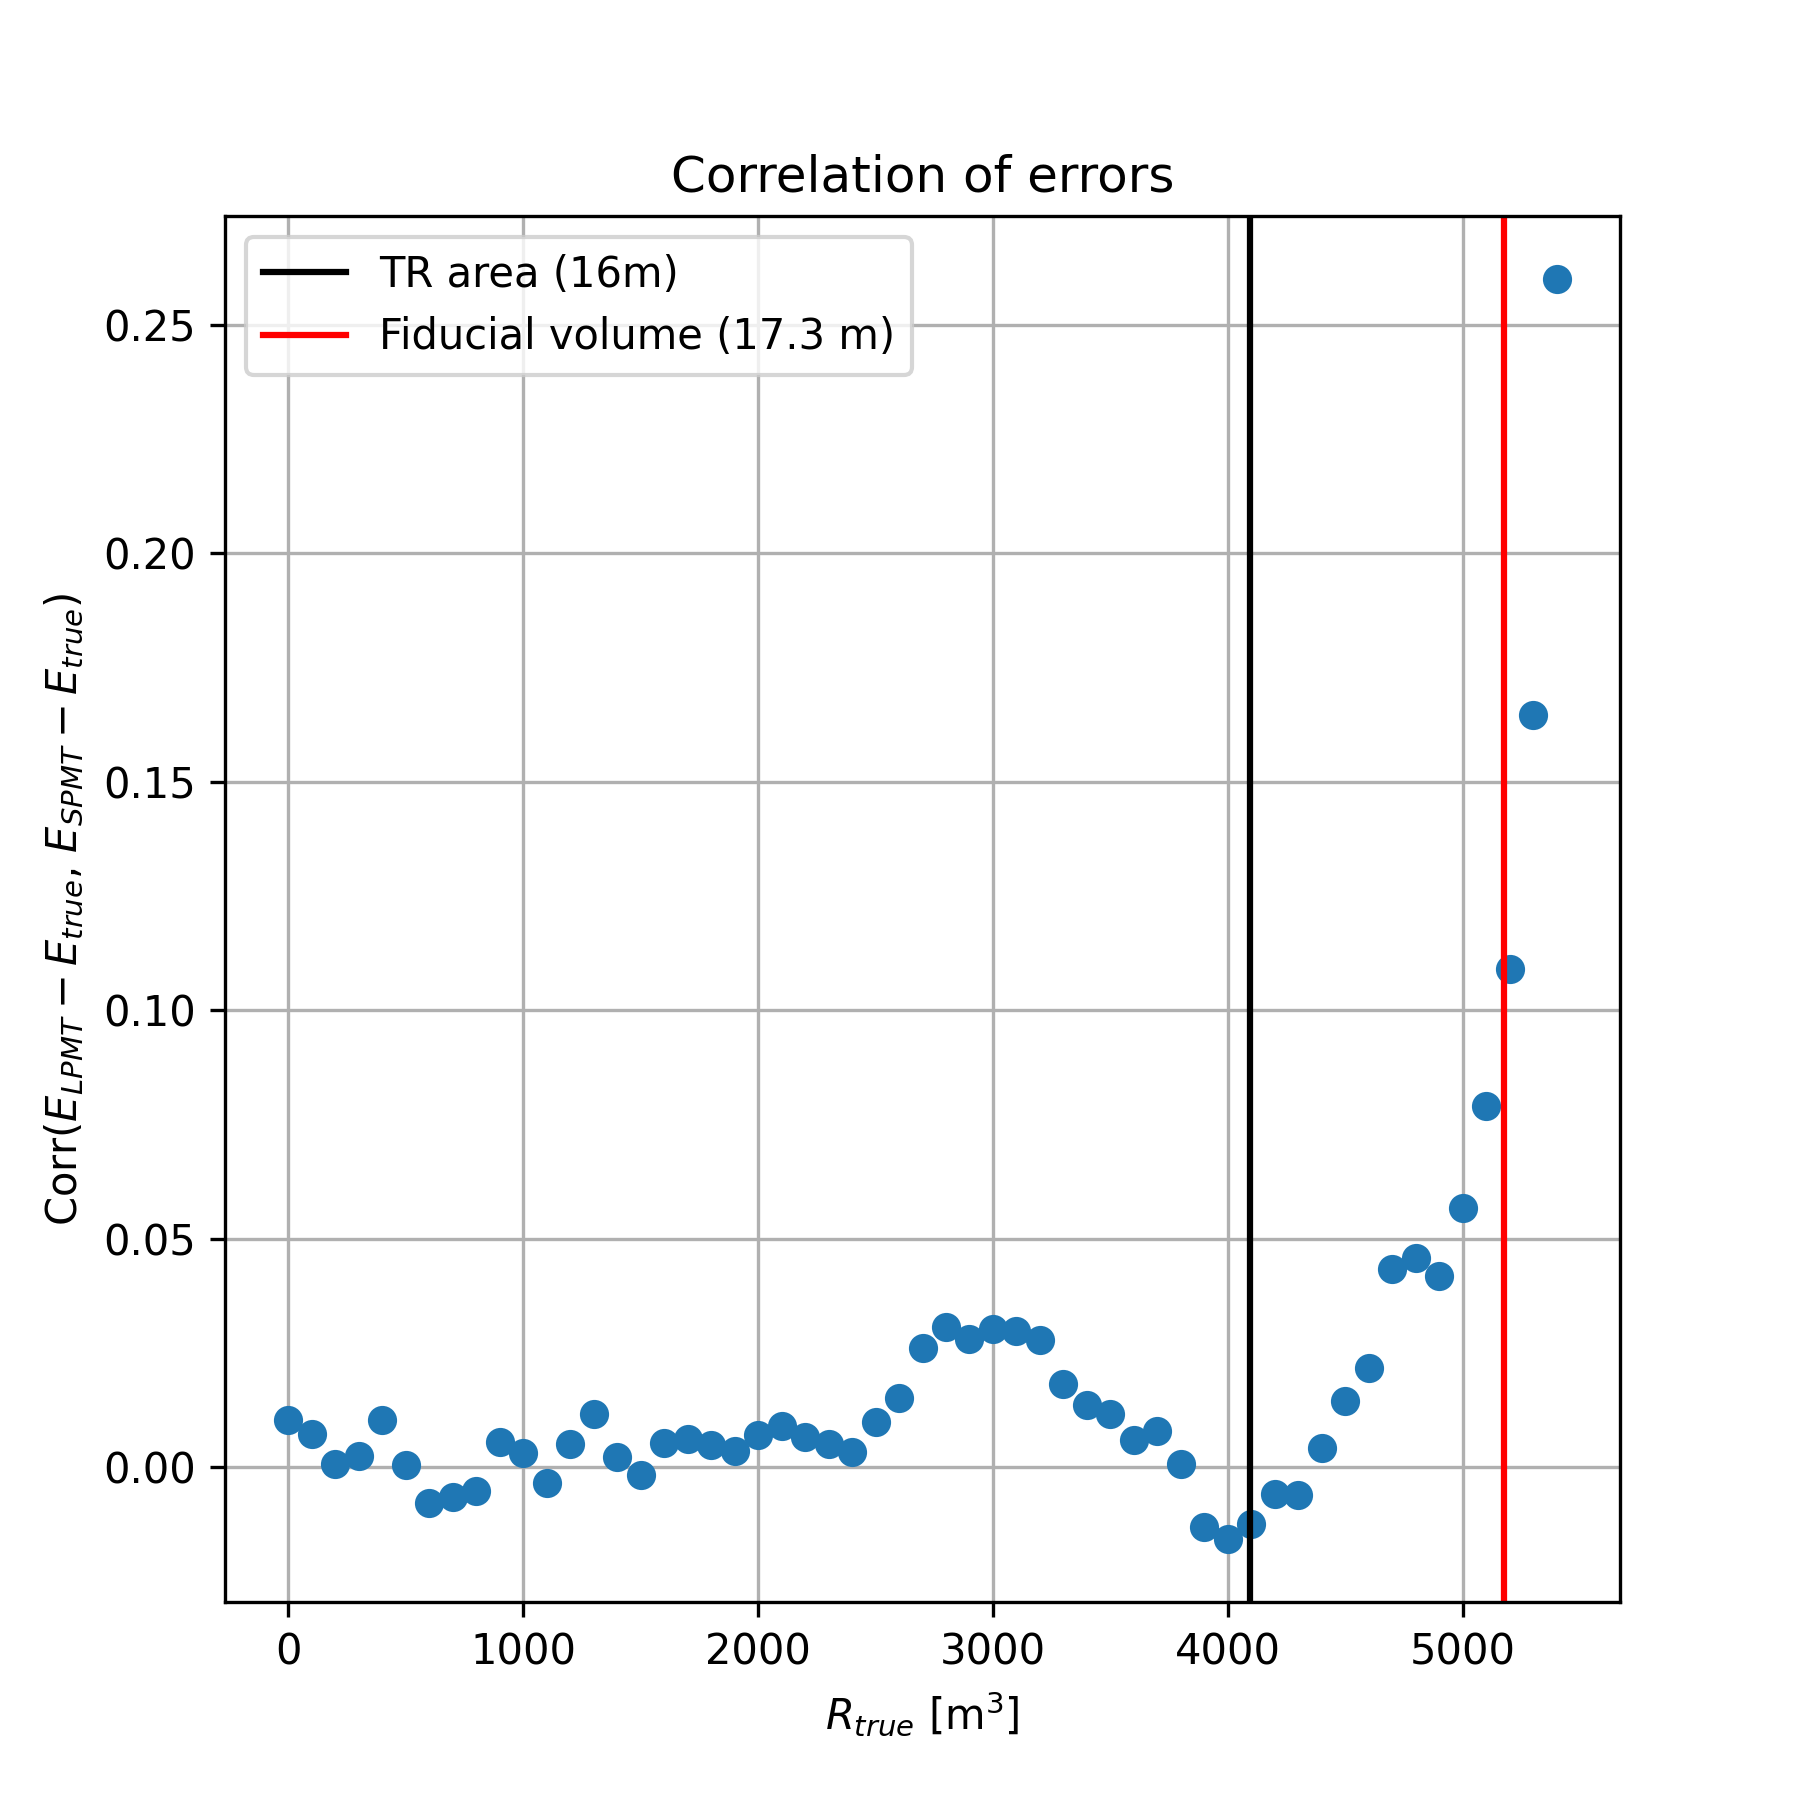
\includegraphics[width=\linewidth]{images/joint_fit/R_corr.png}
  \end{subfigure}
  \caption{Correlation on the reconstruction error between the LPMT and SPMT system as a function of \textbf{(On the left)} the energy, \textbf{(On the right)} the radius. The SPMT reconstruction comes from the NN presented in Chapter \ref{sec:jcnn} and the LPMT reconstruction comes from OMILREC presented in Section \ref{sec:juno:reco}. To prevent effect due to the CNN bad reconstruction, we select the event with $1 < E_{dep} < 9$ MeV.}
  \label{fig:joint_fit:empirical_corr:E_a_R}
\end{figure}

The first observation here is that in most of the detector volume, the correlation between the SPMT and LPMT energy reconstructions does not exceed a few percents, and is in general positive.

In principle, this correlation must be dominated by the fluctuations of the photon yield produced in the scintillator, which dominates the stochastic term of the resolution (see Equation \ref{eq:joint_fit:abc}). Indeed, in a given event, both the LPMT and SPMT reconstruct the energy from the same photon yield and both are affected in the same way by a fluctuation. The correlation is reduced by the fact that SPMT system, due to its low coverage, detect only a very small fraction of the photon. This sampling is also a random phenomenon : the corresponding fluctuations hide to some extent the fluctuations of the original photon yield, and are essentially independent of the random number of photons sampled by the LPMT.

When energy is deposited at high R, close to or in the total reflection area, the proximity of the PMTs increases the number of photons detected by LPMT, and therefore reduce the sampling fluctuations. In this case, the fluctuation of the original photon yield is less shuffled by the sampling fluctuations and the resulting correlation between the LPMT and SPMT reconstruction reaches high values, up to 25\% (Fig. \ref{fig:joint_fit:empirical_corr:E_a_R}, right).

The original photon yield grows with the visible energy. For the same reason as above, the correlation grows as well, albeit far more slowly than as a function of $R^3$. On Fig. \ref{fig:joint_fit:empirical_corr:E_R}, one can see that cumulating the effects of high energy and high $R$, correlations can reach 35\%. However, in the fiducial volume and at energies below 7 MeV (ie in a part of the spectrum containing the sensitivity to $\Delta m^2_{12}$ and $\sin^2(2 \theta_{12})$), it never exceeds 15\%.

\begin{figure}[ht]
  \centering
  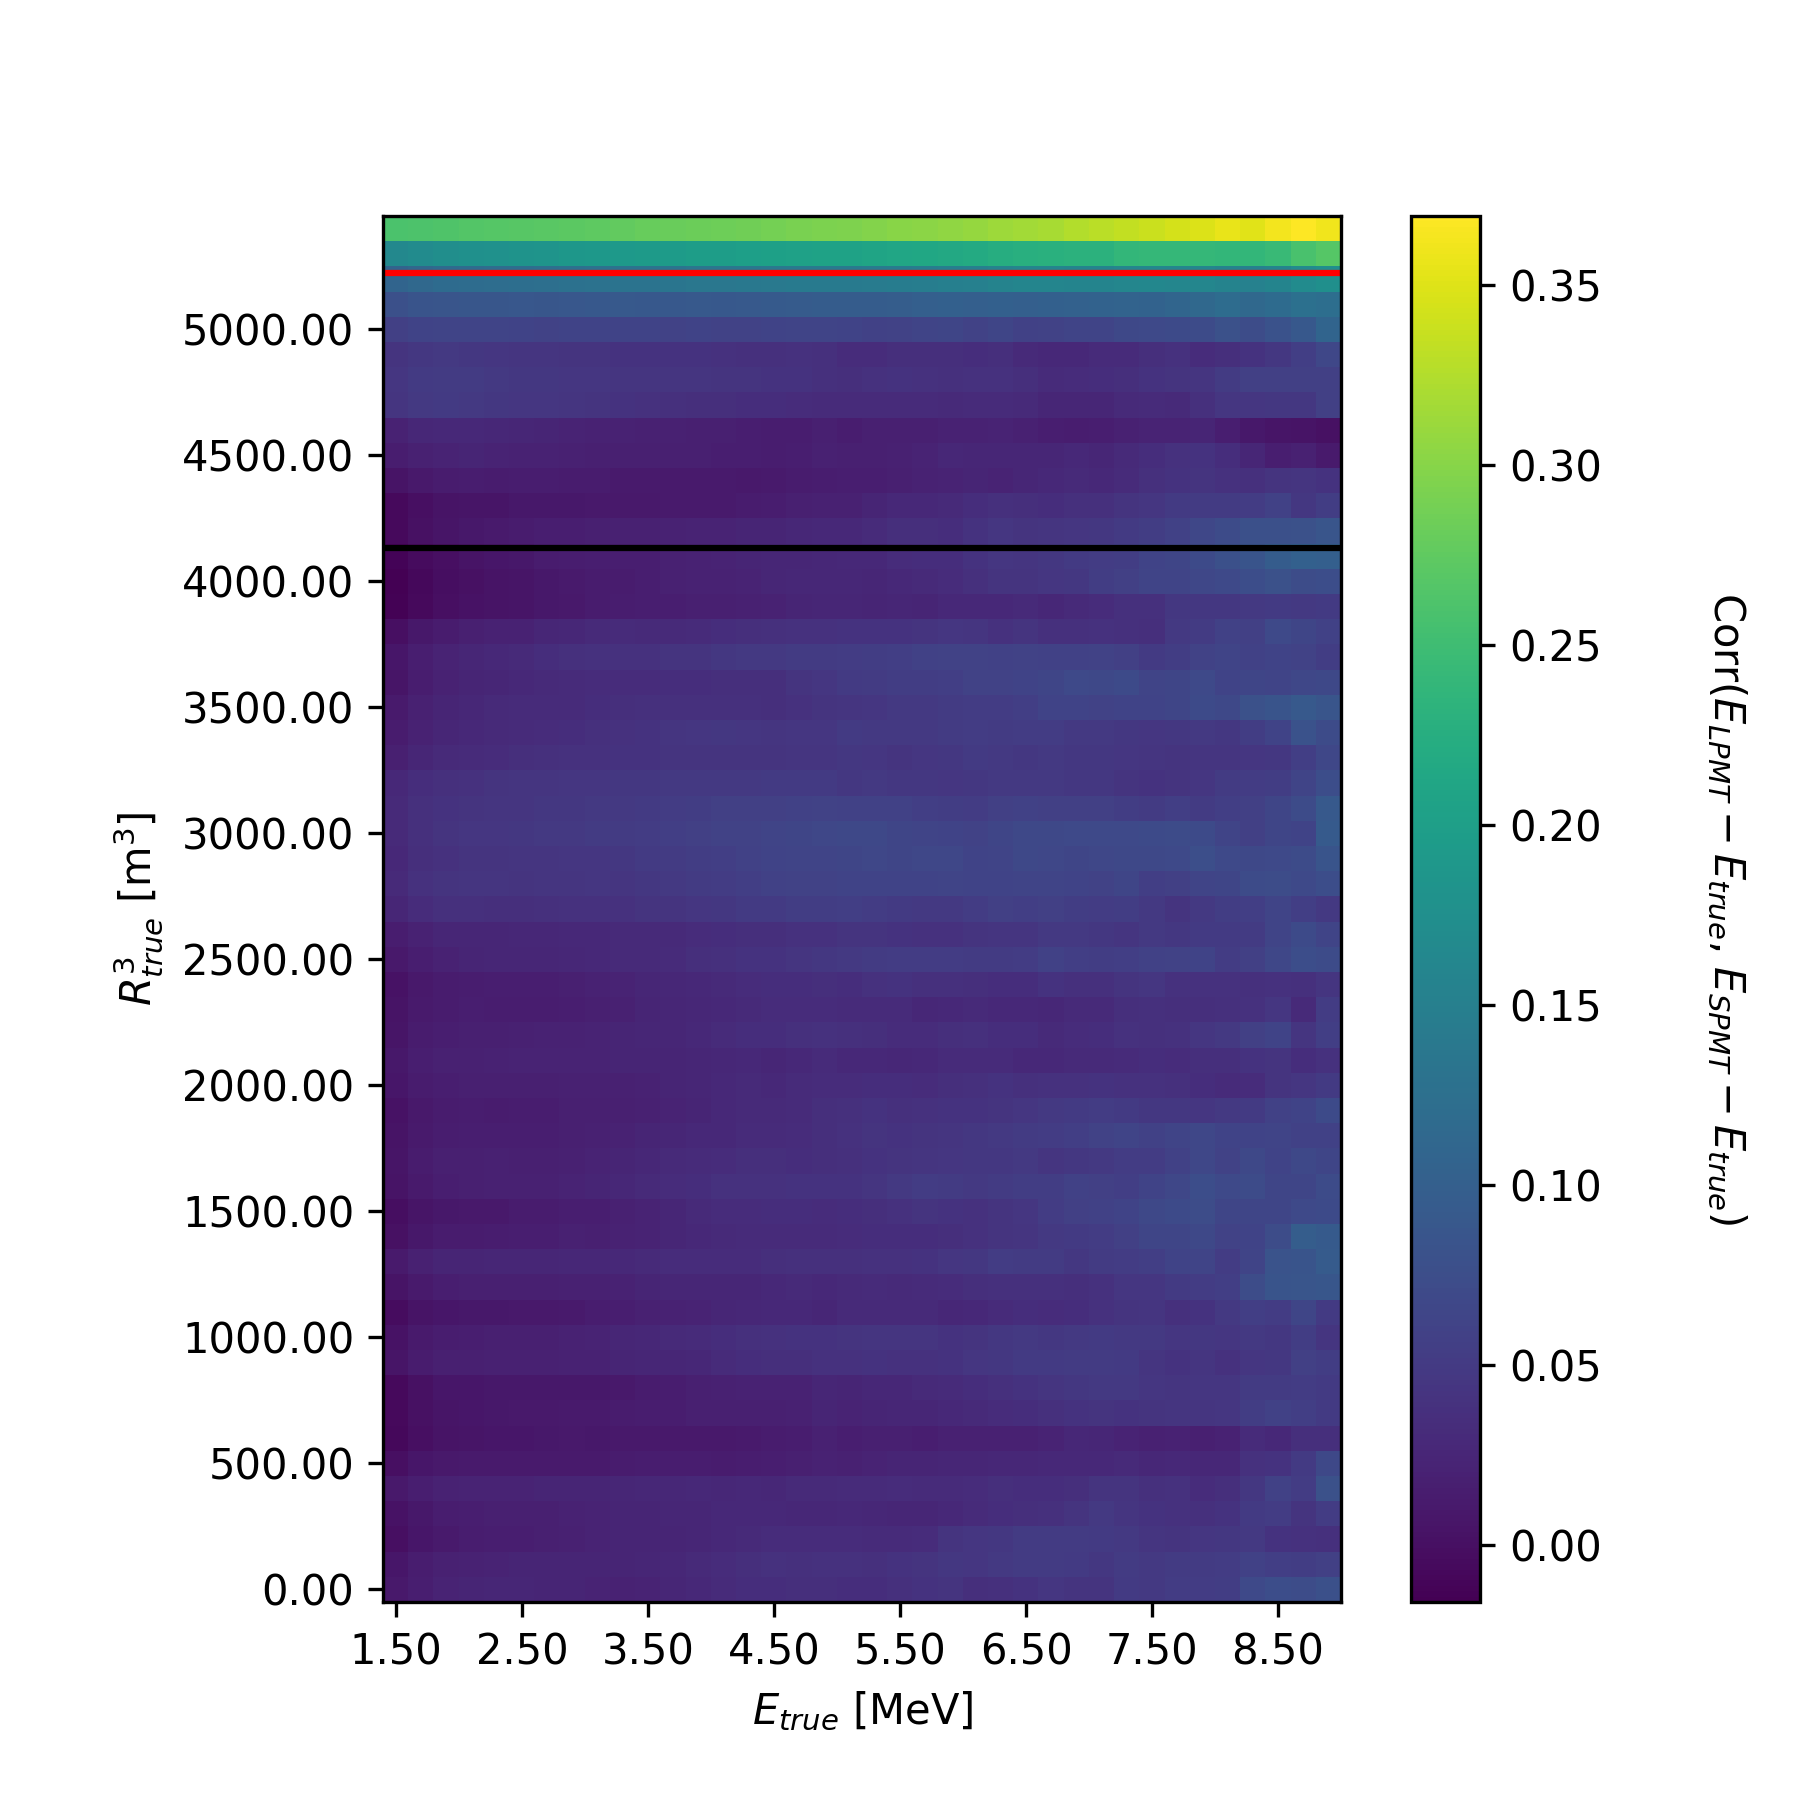
\includegraphics[height=10cm]{images/joint_fit/E_R_corr.png}
  \caption{Correlation on the reconstruction error between the LPMT and SPMT system as a function of  the energy and the radius. The SPMT reconstruction comes from the NN presented in Chapter \ref{sec:jcnn} and the LPMT reconstruction comes from OMILREC presented in Section \ref{sec:juno:reco}. To prevent effect due to the CNN bad reconstruction, we select the event with $1 < E_{dep} < 9$ MeV.}
  \label{fig:joint_fit:empirical_corr:E_R}
\end{figure}

To re-evaluate $V$ with these reconstruction correlations accounted for, we should perform an empiric evaluation (like in Section \ref{sec:joint_fit:cov_mat:emp}).
It would be based on toys generated with the IBD generator (see point 9 of Section \ref{sec:joint_fit:framework:ibd-gen}), replacing the two independent random gaussian drawings by a drawing according to a 2 dimensional gaussian describing the ($E^{lpmt}_{rec}-E_{vis}$) vs. ($E^{spmt}_{rec}-E_{vis}$)  distribution, and involving the correlations studied above.

A way must be found to include the variation of the correlation as a function of $R$ and the $E_{vis}$. We have tried to define 2-dimensional regions in these variables, and defined each time the corresponding 2 dimensional gaussian. Then, we tuned the IBD generator to choose which of these gaussians to sample, based on the generated values of $E_{vis}$ and $R$. Unfortunately, due to the limited statistics of the full simulation sample, the $E_{vis}:R^3$ regions were too wide. It lead to sawtooth variations of the correlation and mean values of the gaussian between neighbouring regions. The reconstructed spectra finally showed irregularities instead of a normal, smooth aspect, making it improper for any oscillation analysis.

Before a solution can be found to this problem, we limit our conclusions to this :

\begin{itemize}
  \item The correlation between the LPMT and SPMT energy reconstruction is positive. Therefore, the SPMT and LPMT spectra should be more correlated than assumed in the statistical tests presented in this chapter. With a proper treatment, we can therefore expect a higher sensitivity to unexpected instrumental effects like QNL.

  \item In 80\% of the detector's volume, reconstruction correlations are low, and should not impact much the sensitivities of our test statistics. If the dependence of the correlation on $E_{vis}$ and $R$ proved too difficult to model, one could cut IBDs reconstructed in the Total reflection area. The loss in statistics would be limited, as well as the impact on the sensitivities of the statistical tests.
\end{itemize}

Additionally, this study is preliminary, as the background was neglected in the distortion test, and no systematic uncertainties were considered. Those points could be easily addressed by regenerating background spectra using the same reference as used by JUNO for the common inputs and by regenerating the systematic covariances matrix with both LPMT and SPMT spectra.

The supplementary non-linearity was introduced event-wise but should be applied channel-wise to account for the detector's non-uniformity. This can be addressed via generating oscillated spectra through the JUNO official simulation. This process is very time consuming and require technical development but could be achievable given enough time.

The correlation matrix between the LPMT and SPMT spectra should also be further analyzed, as indicated by the discrepancies between the theoretical and empirical correlation matrices.

\end{document}
